%----------
%   WARNING
%----------

% This Guide contains Library recommendations based mainly on APA and IEEE styles, but you must always follow the guidelines of your TFG Tutor and the TFG regulations for your degree.

% THIS TEMPLATE IS BASED ON THE IEEE STYLE 


%----------
% DOCUMENT SETTINGS
%----------

\documentclass[12pt]{report} % font: 12pt

% margins: 2.5 cm top and bottom; 3 cm left and right
\usepackage[
a4paper,
vmargin=2.5cm,
hmargin=3cm
]{geometry}

% Paragraph Spacing and Line Spacing: Narrow (6 pt / 1.15 spacing) or Moderate (6 pt / 1.5 spacing)
\renewcommand{\baselinestretch}{1.15}
\parskip=6pt

% Color settings for cover and code listings 
\usepackage[table]{xcolor}
\definecolor{azulUC3M}{RGB}{0,0,102}
\definecolor{gray97}{gray}{.97}
\definecolor{gray75}{gray}{.75}
\definecolor{gray45}{gray}{.45}

\usepackage{enumerate}

% PDF/A -- Important for its inclusion in e-Archive. PDF/A is the optimal format for preservation and for the generation of metadata: http://uc3m.libguides.com/ld.php?content_id=31389625. 

% In the template we include the file OUTPUT.XMPDATA. You can download that file and include the metadata that will be incorporated into the PDF file when you compile the memoria.tex file. Then upload it back to your project.  
\usepackage[a-1b]{pdfx}

% LINKS
\usepackage{hyperref}
\hypersetup{colorlinks=true,
	linkcolor=blue, % links to parts of the document (e.g. index) in black (changed because a black link in a black text does not make any sense whatsoever)
	urlcolor=blue} % links to resources outside the document in blue

% MATH EXPRESSIONS
\usepackage{amsmath,amssymb,amsfonts,amsthm}

\newcommand*{\mynum}[1]{\num[output-decimal-marker={.},
                             round-mode=places,
                             round-precision=2,
                             group-digits=false]{#1}}

\newtheorem{definition}{Definition}
\newtheorem{theorem}{Theorem}
\newtheorem{problem}{Problem}
\newtheorem{example}{Example}
\newtheorem{corollary}{Corollary}
\newtheorem{lemma}{Lemma}
\newtheorem{remark}{Remark}


% Character encoding
\usepackage{txfonts} 
\usepackage[T1]{fontenc}
\usepackage[utf8]{inputenc}

% English settings
\usepackage[english]{babel} 
\usepackage[babel, english=american]{csquotes}
\AtBeginEnvironment{quote}{\small}

\usepackage{todonotes}
\usepackage{wrapfig}
% Footer settings
\usepackage{fancyhdr}
\pagestyle{fancy}
\fancyhf{}
\renewcommand{\headrulewidth}{0pt}
\rfoot{\thepage}
\fancypagestyle{plain}{\pagestyle{fancy}}

% DESIGN OF THE TITLES of the parts of the work (chapters and epigraphs or sub-chapters)
\usepackage{titlesec}
\usepackage{titletoc}
\titleformat{\chapter}[block]
{\large\bfseries\filcenter}
{\thechapter.}
{5pt}
{\MakeUppercase}
{}
\titlespacing{\chapter}{0pt}{0pt}{*3}
\titlecontents{chapter}
[0pt]                                               
{}
{\contentsmargin{0pt}\thecontentslabel.\enspace\uppercase}
{\contentsmargin{0pt}\uppercase}                        
{\titlerule*[.7pc]{.}\contentspage}                 

\titleformat{\section}
{\bfseries}
{\thesection.}
{5pt}
{}
\titlecontents{section}
[5pt]                                               
{}
{\contentsmargin{0pt}\thecontentslabel.\enspace}
{\contentsmargin{0pt}}
{\titlerule*[.7pc]{.}\contentspage}

\titleformat{\subsection}
{\normalsize\bfseries}
{\thesubsection.}
{5pt}
{}
\titlecontents{subsection}
[10pt]                                               
{}
{\contentsmargin{0pt}                          
	\thecontentslabel.\enspace}
{\contentsmargin{0pt}}                        
{\titlerule*[.7pc]{.}\contentspage}  


% Tables and figures settings
\usepackage{multirow} % combine cells 
\usepackage{caption} % customize the title of tables and figures
\usepackage{floatrow} % we use this package and its \ ttabbox and \ ffigbox macros to align the table and figure names according to the defined style.
\usepackage{array} % with this package we can define in the following line a new type of column for tables: custom width and centered content
\newcolumntype{P}[1]{>{\centering\arraybackslash}p{#1}}
\DeclareCaptionFormat{upper}{#1#2\uppercase{#3}\par}
\usepackage{graphicx}
\graphicspath{{imagenes/}} % Images folder

% Table layout for engineering
\captionsetup*[table]{
	format=upper,
	name=TABLE,
	justification=centering,
	labelsep=period,
	width=.75\linewidth,
	labelfont=small,
	font=small
}

% Figures layout for engineering
\captionsetup[figure]{
	format=hang,
	name=Fig.,
	singlelinecheck=off,
	labelsep=period,
	labelfont=small,
	font=small		
}

% FOOTNOTES
\usepackage{chngcntr} % continuous numbering of footnotes
\counterwithout{footnote}{chapter}

% CODE LISTINGS 
% support and styling for listings. More information in  https://es.wikibooks.org/wiki/Manual_de_LaTeX/Listados_de_código/Listados_con_listings
\usepackage{listings}

% Custom listing
\lstdefinestyle{estilo}{ frame=Ltb,
	framerule=0pt,
	aboveskip=0.5cm,
	framextopmargin=3pt,
	framexbottommargin=3pt,
	framexleftmargin=0.4cm,
	framesep=0pt,
	rulesep=.4pt,
	backgroundcolor=\color{gray97},
	rulesepcolor=\color{black},
	%
	basicstyle=\ttfamily\footnotesize,
	keywordstyle=\bfseries,
	stringstyle=\ttfamily,
	showstringspaces = false,
	commentstyle=\color{gray45},     
	%
	numbers=left,
	numbersep=15pt,
	numberstyle=\tiny,
	numberfirstline = false,
	breaklines=true,
	xleftmargin=\parindent
}

\usepackage[normalem]{ulem}
\captionsetup*[lstlisting]{font=small, labelsep=period}
 
\lstset{style=estilo}
\renewcommand{\lstlistingname}{\uppercase{Code}}


% REFERENCES 

% IEEE bibliography setup
\usepackage[backend=biber, style=ieee, isbn=false,sortcites, maxbibnames=6, minbibnames=1]{biblatex} % Setting for IEEE citation style, recommended for engineering. "maxbibnames" indicates that from 6 authors truncate the list in the first one (minbibnames) and add "et al." as used in the IEEE style.

\addbibresource{referencias.bib} % The references.bib file in which the bibliography used should be

\usepackage{graphbox}
% start TeXmacs macros
\newcommand{\nobracket}{}
\newcommand{\tmmathbf}[1]{\ensuremath{\boldsymbol{#1}}}
\newcommand{\tmem}[1]{{\em #1\/}}
\newcommand{\tmop}[1]{\ensuremath{\operatorname{#1}}}
\newcommand{\tmstrong}[1]{\textbf{#1}}
\newcommand{\tmverbatim}[1]{\text{{\ttfamily{#1}}}}
\providecommand{\xequal}[2][]{\mathop{=}\limits_{#1}^{#2}}
\newcommand{\tmcolor}[2]{{\color{#1}{#2}}}
\newcommand{\mathLaplace}{\Delta}
\hfuzz=60.0pt 
% end TeXmacs macros
\usepackage{pdfpages}

%-------------
%	DOCUMENT
%-------------

\begin{document}
\pagenumbering{roman} % Roman numerals are used in the numbering of the pages preceding the body of the work.

%----------
%	COVER
%----------	
\begin{titlepage}
  \begin{sffamily}
    \color{azulUC3M}
    \begin{center}
      \begin{figure}[ht] % UC3M Logo
        \makebox[\textwidth][c]{
\includegraphics[width=16cm]{logo_UC3M.png}}
      \end{figure}
      \vspace{2.5cm}
      \begin{Large}
        Master Degree in Computational and Applied Mathematics\\
        2023-2024\\ % Academic year
        \vspace{2cm}
        \textsl{Master Thesis}
        \bigskip

      \end{Large}
      {\Huge ``Thesis title''}\\
      \vspace*{0.5cm}
      \rule{10.5cm}{0.1mm}\\
      \vspace*{0.9cm}
      {\LARGE Héctor Rodrigo Iglesias Goldaracena}\\
      \vspace*{1cm}
      \begin{Large}
        1st Víctor Bayona Revilla\\
        2nd Pedro González Rodríguez\\
        Place and date\\
      \end{Large}
    \end{center}
    \vfill
    \color{black}
    \fbox{
      \begin{minipage}{\linewidth}
        \textbf{AVOID PLAGIARISM}\\
        \footnotesize{The University uses the \textbf{Turnitin Feedback Studio} for the delivery of student work. This program compares the originality of the work delivered by each student with millions of electronic resources and detects those parts of the text that are copied and pasted. Plagiarizing in a TFM is considered a  \textbf{\underline{Serious Misconduct}}, and may result in permanent expulsion from the University.}\end{minipage}}

    % IF OUR WORK IS TO BE PUBLISHED UNDER A CREATIVE COMMONS LICENSE, INCLUDE THESE LINES. IS THE RECOMMENDED OPTION.
    \noindent
\includegraphics[width=4.2cm]{creativecommons.png}\\ % Creative Commons Logo
    \footnotesize{This work is licensed under Creative Commons \textbf{Attribution – Non Commercial – Non Derivatives}}

  \end{sffamily}
\end{titlepage}

\newpage % blank page
\thispagestyle{empty}
\mbox{}

\newpage % blank page
\thispagestyle{empty}
\mbox{}

%----------
%	ABSTRACT AND KEYWORDS 
%----------	
\renewcommand\abstractname{\large\bfseries\filcenter\uppercase{Summary}}
\begin{abstract}
  \thispagestyle{plain}
  \setcounter{page}{3}

  % Write your abstract

  \textbf{Keywords:} % add the keywords

  \vfill
\end{abstract}
\newpage % Blank page
\thispagestyle{empty}
\mbox{}


%----------
%	Dedication
%----------	
% \chapter*{Dedication}

\setcounter{page}{5}

% Write here	

\vfill

\newpage % blank page
\thispagestyle{empty}
\mbox{}


%----------
%	TOC
%----------	

%--
% TOC
%-
\tableofcontents
\thispagestyle{fancy}

\newpage % blank page
\thispagestyle{empty}
\mbox{}

%--
% List of figures. If they are not included, comment the following lines
%-
\listoffigures
\thispagestyle{fancy}

\newpage % blank page
\thispagestyle{empty}
\mbox{}

%--
% List of tables. If they are not included, comment the following lines
%-
\listoftables
\thispagestyle{fancy}

\newpage % blankpage
\thispagestyle{empty}
\mbox{}


%----------
%	THESIS
%----------	
\clearpage
\pagenumbering{arabic} % numbering with Arabic numerals for the rest of the document.	

\chapter{Introduction}
% \section{Motivation}

Machine Learning (ML) has experienced a surge in popularity and application across various
domains in recent years, which can be owed to different contributing factors.
Firstly, the development of now readily available high performance hardware like
Graphics Processing Units (GPUs) has significantly sped up the times of training
and inference of ML models, where
repeated operations are common \cite{oh2004gpu}.
Moreover, algorithmic improvements like automatic differentiation has enabled a streamlined
way to find suitable parameters for models solving a wide variety of problems
\cite{baydin2018automatic}.

A second contributing factor is data availability. Be it social media,
embedded hardware sensors or any of our technological devices, a copious amount of data
is produced
by the minute which can then be labored by ML algorithms to identify patterns and
make predictions. Not only that, governments worldwide are fostering open access to
data across domains as varied as culture, demography, environment and technology.
In particular, the government of Spain, the country where this Master's thesis has been
written in, is undertaking efforts in the framework of their
\href{https://datos.gob.es/en}{Open Data initiative} to leverage collaboration between
analysts and contributing to the spread of knowledge.

Precisely along this last idea, the third key contributing factor is found in the form
of Free and Open Source Software (FOSS). The open nature of ML libraries like
\href{https://pytorch.org/}{PyTorch} and \href{https://www.tensorflow.org/}{TensorFlow}
have not only made state-of-the-art
techniques accessible to the broad public, but also seen the benefits entailing any FOSS
project: volunteers and professionals alike freely
contributing in a transparent environment
to the improvement, triaging, interoperability and other extensions of these projects.

Despite its widespread adoption and empirical success, a robust theoretical foundation that
guarantees the effectiveness of ML is still lacking, while empirical evidence abounds
regarding its usefulness across multiple areas of knowledge.

One notable characteristic of ML models is their inherent complexity, which often manifests
in intricate model architectures and parameter configurations \cite{cuomo2022scientific}.
The currently heuristic nature of ML techniques stands in the way of decisively
anticipating if a given model will be up to the task at hand.
Indeed, while it is true that one can always verify if the inputs of
the model suit the problem parameters and if the output of the model suits the solution,
providing a justification of the effectiveness of each intermediate layer that is
exempt of heuristics is a non-trivial task.

Drawing parallels with classical numerical methods, such as the finite element method (FEM) for
solving partial differential equations (PDEs), provides valuable insights into the underlying
principles of some models in ML. In the former framework,
basis functions are employed to
reconstruct the target function through a linear combination, akin to the linear combination
one would expect to find at the last layer of many neural networks.

However, a fundamental distinction arises in the
prescription of basis functions: while numerical methods explicitly define basis functions,
such as ``hat'' functions for solving ordinary differential equations (ODEs), ML practitioners
rely on arbitrarily complex compositions of functions which have been empirically verified
to possess sufficient approximation capacity for the desired problem domains.

Latent similarities between FEM (as well as other techniques) and ML practices
can potentially show the way forward to reconciling well-known theoretical principles with
surging empirical methodologies. While numerical
methods offer rigorous formulations and verifiable procedures, ML adopts a more heuristic
approach by leveraging compositions of functions with empirically validated approximation
capabilities.

The aim of this work is to establish an intermediary perspective that intertwines
mathematical theory, particularly that of Radial Basis Functions (RBFs), with the
computational power and flexibility supplied by ML techniques.


\section{Objectives}

\chapter{State of the art}
\section{Neural Networks} \label{sec-neural-networks}
The starting point for defining a Neural Network is the multilayer perceptron, whose recursive definition we express following \cite{lu2021deepxde}:
\begin{definition}[Multilayer perceptron]
  Let \(L \in \mathbb{N}\) and \(\{ N_i \}_{i = 1}^L \subset \mathbb{N}\). The
    {\textbf{$L-$layer perceptron}} is a function
  \begin{equation}
    \begin{array}{llll}
      \mathcal{N}^L : & \mathbb{R}^{N_0} & \rightarrow     & \mathbb{R}^{N_L}                   \\
                      & \tmmathbf{x}     & \hookrightarrow & \tmmathbf{W}^L \mathcal{N}^{L - 1}
      (\tmmathbf{x}) +\tmmathbf{b}^L
    \end{array},
    \label{perceptronRule}
  \end{equation}
  % \[ \begin{array}{llll}
  %      \mathcal{N}^L : & \mathbb{R}^{N_0} & \rightarrow & \mathbb{R}^{N_L}\\
  %      & \tmmathbf{x} & \hookrightarrow & \tmmathbf{W}^L \mathcal{N}^{L - 1}
  %      (\tmmathbf{x}) +\tmmathbf{b}^L
  %    \end{array}, \]
  where \(\mathcal{N}^{L - 1} : \mathbb{R}^{N_0} \rightarrow \mathbb{R}^{N_{L- 1}}\) is defined according to the rule
  \[ \mathcal{N}^{L - 1} (\tmmathbf{x}) = \left\{\begin{array}{ll}
      \tmmathbf{x},           & \text{if } L = 1 \\
      \sigma_{L - 1} (\tmmathbf{W}^{L - 1} \mathcal{N}^{L - 2} (\tmmathbf{x})
      +\tmmathbf{b}^{L - 1}), & \text{otherwise}
    \end{array}\right. . \]
  We shall refer to some \(\tmmathbf{b}^i \in \mathbb{R}^{\mathbb{N}_i}, 1 \leq i \leq L\) as the {\textbf{bias}} of the \(i -\)th layer, and each
  \(\tmmathbf{W}^i \in \mathbb{R}^{N_i \times N_{i - 1}}\) as the
  \textbf{weights matrix} of the \(i -\)th layer. Finally, the \textbf{activation function} of the $i
    -$th layer, \(\sigma_i\), is commonly defined as
  \[ \begin{array}{cccc}
      \sigma_i : & \mathbb{R}^{\mathbb{N}_i} & \rightarrow     &
      \mathbb{R}^{\mathbb{N}_i}                                                               \\
                 & (x_1, x_2, \ldots, x_i)   & \hookrightarrow & (\phi_i (x_1), \phi_i (x_2),
      \ldots, \phi_i (x_n))
    \end{array} \]
  that is, the element-wise application of some function
  $\phi_i$.

  The multilayer perceptron is also named \textbf{feedforward network}.
\end{definition}

Some common activation function choices are the sigmoid function, $x \mapsto 1/(1 + e^{- x})$, the hyperbolic tangent, $x \mapsto (e^x - e^{- x})/(e^x + e^{- x})$ and the Rectified Linear Unit (ReLU), $x \mapsto \max \{ 0, x \}$.

Contrary to what one may instinctively think, the $1 -$layer perceptron equipped with a suitable activation function is
enough to characterize any continuous function, that is, it is
  {\tmstrong{dense}} in the space of continuous functions of $n \text{
    variables, } C (I_n)$. We briefly quote the terminology and formulation
proposed by Cybenko in \cite{cybenko1989approximation}, where a proof of this result can be found.

\begin{definition}[Discriminatory function]
  Let $M (I_n)$ denote the space of finite, signed regular measures on \(I_n\).
  A function \(\sigma\) is said to be {\tmstrong{discriminatory}} if for a
  measure \(\mu \in M (I_n)\) we have that
  \[ \int_{I_n} \sigma (y^{\top} x + \theta) d \mu (x) = 0 \text{ for all } y
    \in \mathbb{R}^n, \theta \in \mathbb{R} \]
  implies that \(\mu = 0\).
  % Moreover, a function $t \mapsto \sigma (t)$ is said
  % to be {\tmstrong{sigmoidal}} if
  % \[ \lim_{t \rightarrow + \infty} \sigma (t) = 1, \text{ and } \lim_{t
  % \rightarrow - \infty} \sigma (t) = 0. \]
\end{definition}

\begin{theorem}[Universal approximation]
  Let \(\sigma\) be any continuous discriminatory function. Then, finite sums of
  the form
  \[ G (x) = \sum_{j = 1}^N \alpha_j \cdot \sigma (y_j^{\top} x + \theta_j) \]
  are dense in \(C (I_n)\), i.e., for any $\varepsilon > 0 \text{ and } f \in C
    (I_n)$ we can find a sum \(G (x)\) such that
  \[ | G (x) - f (x) | < \varepsilon \text{, for } x \in I_n . \]
\end{theorem}



\section[PINNs]{PINNs\footnote{Throughout this section, we shall follow the order of presentation proposed in \cite{cuomo2022scientific}.}}\label{section:pinns}

Physics-Informed Neural Networks (PINNs in the following) constitute the
machine learning techniques that are used to solve Partial Differential
Equations, which are problems of the form
\begin{equation}
  (P) = \left\{\begin{array}{rlll}
    F (u (\tmmathbf{z}) ; \gamma) & = & f (\tmmathbf{z}), & \tmmathbf{z} \in
    \Omega                                                                            \\
    B (u (\tmmathbf{z}))          & = & g (\tmmathbf{z}), & \tmmathbf{z} \in \partial
    \Omega
  \end{array}\right. \label{pdegeneralform}
\end{equation}
where we consider the open set $\Omega \subset \mathbb{R}^d$ whose boundary is
denoted $\partial \Omega$, with $\tmmathbf{z}= (\tmmathbf{x}, t)$. Moreover,
\(F\) is a non-linear differential operator whose arguments are the solution $u$
we want to find, up to some model parameters $\gamma$ and prescribed to be
equal to our problem data \(f\). Finally, \(B\) is an operator which can denote
initial (\(t = 0\)) or boundary conditions. For instance, if $B$ is set to be
the identity operator (resp., gradient operator) we recover Dirichlet (resp.,
Neumann) boundary conditions.

Provided $\gamma$ is known, the process of finding $u$ is called
  {\tmstrong{forward}} problem\footnote{We shall focus the rest of the
  discussion on problems of this form.}. Reciprocally, if $\gamma$ is to be
determined alongside $u$ up to particular measurements of the problem under study, the problem is called {\tmstrong{inverse}}. Under
the PINN framework, and denoting by $(\tmmathbf{z}, \theta) \mapsto
  \mathcal{N}\mathcal{N} (\tmmathbf{z}; \theta)$ an arbitrary neural network of input $\tmmathbf{z}$ and
parameters $\theta$, we intend to find suitable $\hat{ \theta}$ such that
$\mathcal{N}\mathcal{N} (\tmmathbf{z}; \hat{ \theta}) \simeq u (\tmmathbf{z})$. The
usual work plan involves finding
\begin{equation}
  \arg \min_{\theta} \mathcal{L} (\theta) = \arg \min_{\theta} \omega_F
  \mathcal{L}_F (\theta) + \omega_B \mathcal{L}_B (\theta),
  \label{loss-fun-pinn}
\end{equation}
where
\begin{equation}
  \mathcal{L}_F (\theta) = \int_{\Omega} (F (\mathcal{N}\mathcal{N}
  (\tmmathbf{z}; \theta)) - f (\tmmathbf{z}))^2 d\tmmathbf{z},
  \label{loss-F}
\end{equation}
and
\begin{equation}
  \mathcal{L}_B (\theta) = \int_{\partial \Omega} (B (\mathcal{N}\mathcal{N}
  (\tmmathbf{z}; \theta)) - g (\tmmathbf{z}))^2 d\tmmathbf{z}
  \label{loss-boundary}
\end{equation}
which come usually prescribed as mean square errors in the corresponding
discretized form. Finally, $\omega_F$, $\omega_B$ are weights that account for the
reliability of the PDE and how strictly we need the boundary conditions to be
satisfied, respectively.

One question that needs addressing is the computation of $F
  (\mathcal{N}\mathcal{N} (z ; \theta))$. To do so, we first briefly recall the
differentiation techniques that are often studied in undergraduate courses:
\begin{itemize}
  \item The most elementary one is simply computing them by hand. This allows
        us to obtain analytical expressions that can be directly programming into
        the code we are developing to solve some problem, which saves us the
        computation times that come from differentiating.

  \item After a course in numerical methods, {\tmstrong{finite
              differentiation}} is introduced as an easy to program alternative: it
        proposes the discretization of the problem domain, generating a point set
        with as many dimensions as required by the problem. On this set, we apply
        known formulae to approximate the derivatives of the function we intend to
        study.

        A relevant disadvantage of this method is that the grid has to be stored in memory, which poses an upper
        limit to the amount of points we can sample. Another drawback is that the finite differences method decreases its performance as the
        dimension of the problem increases. Indeed, let $f : \mathbb{R}^d
          \rightarrow \mathbb{R}$ be a differentiable function. Considering the 1-step
        forward finite difference formula for a common step $h$, its partial
        derivative $\frac{\partial f}{\partial x_i}$ is computed by evaluating $f
          (x_1, \ldots, x_i, \ldots, x_d)$ and $f (x_1, \ldots, x_i + h, \ldots,
          x_d)$. Consequently, the computation of just the first $n$ partial
        derivatives of $y$ already involves $d + 1$ computations.

  \item Finally, {\tmstrong{symbolic differentiation}} corresponds to the
        differentiation techniques proportioned by the \href{https://www.mathworks.com/help/symbolic/index.html?s\_tid=CRUX\_lftnav}{Matlab Symbolic Toolbox} or \href{https://www.sympy.org/en/index.html}{SymPy}.
        It allows the user to work with the so-called symbolic variables, which
        stand for the usual variables $x, y, z, t$ we use to define functions or
        solve equations. Symbolic differentiation of a function returns another
        function, which completely avoids the problem of numerical approximations.
        However, it is a memory intensive and slow approach.
\end{itemize}

There is a fourth method, called \textbf{automatic differentiation}. This term refers to a set of techniques that exploit the chain rule to evaluate the differential of a given function to machine precision, that is, the differential is as precise as the floating point system we are using on the computing device. This technique also stems from the fact that, in its simplest terms, computer-assisted computations feature elemental functions such as the sine or exponential, as well as elementary arithmetic operations like the sum or product \cite{verma2000introduction}.

To preserve the relevancy of the discussion, we turn to a short example for illustrating automatic differentiation using the so-called ``reverse mode'', which is present in current machine learning software packages such as PyTorch or TensorFlow.

Consider the function $f (x_1, x_2) = e^{2 x_1} - \cos (x_1 x_2)$, which we
shall apply reverse mode automatic differentiation on. This function can be
written as per the scheme in Figure \ref{fig:wengert-trace}, which is also referred to
as the Wengert trace.

\begin{figure}[ht]
  \centering
  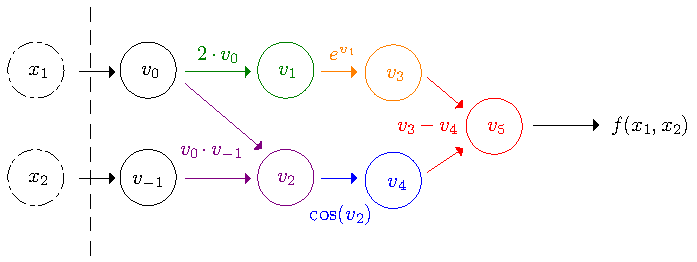
\includegraphics[width=\textwidth]{imagenes/wengert-trace.pdf}
  \caption{Wengert's trace of the function proposed as an example.}
  \label{fig:wengert-trace}
\end{figure}

Assuming that $x_1 = 2, x_2 = 3$, the evaluation of the function according to
the previous graph (i.e., evaluating from left to right) yields $v_0 = 2, v_{-
      1} = 3, v_1 = 4, v_2 = 6, v_3 \simeq 54.60, v_4 \simeq 0.96, v_5 \simeq
  53.64$. Reverse mode automatic differentiation traverses the trace in
``reverse'' order, starting off $f (x_1, x_2)$ and working our way back to
$v_0$ and $v_{- 1}$. This operation is similar to a breadth-first search,
whereby we apply the chain rule and then plug in the values we have for all
our $v$'s. If the trace is to be regarded like a tree, we can separate the
evaluation of these operations in levels:
\begin{itemize}
  \item First level
        \[ \tmcolor{red}{\frac{\partial f}{\partial v_5}} = \frac{\partial
            f}{\partial f} = 1 \]
  \item Second level
        \[ \tmcolor{orange}{\frac{\partial f}{\partial v_3}} =
          \tmcolor{red}{\frac{\partial f}{\partial v_5}} \cdot \frac{\partial
            v_5}{\partial v_3} = \tmcolor{red}{\frac{\partial f}{\partial v_5}} \cdot
          \frac{\partial (v_3 - v_4)}{\partial v_3} = 1, \quad
          \tmcolor{blue}{\frac{\partial f}{\partial v_4}} =
          \tmcolor{red}{\frac{\partial f}{\partial v_5}} \cdot \frac{\partial
            v_5}{\partial v_4} = \tmcolor{red}{\frac{\partial f}{\partial v_5}} \cdot
          \frac{\partial (v_3 - v_4)}{\partial v_4} = - 1 \]
  \item Third level
        \[ {\color[HTML]{008000}\frac{\partial f}{\partial v_1}} =
          \tmcolor{orange}{\frac{\partial f}{\partial v_3}} \cdot \frac{\partial
            v_3}{\partial v_1} = 1 \cdot \frac{\partial (e^{v_1})}{\partial v_1} =
          e^{v_1} \simeq 54.60, \quad {\color[HTML]{800080}\frac{\partial
              f}{\partial v_2}} = \tmcolor{blue}{\frac{\partial f}{\partial v_4}} \cdot
          \frac{\partial v_4}{\partial v_2} = - \frac{\partial v_4}{\partial v_2} =
          \sin (v_2) \simeq - 0.28 \]
  \item Fourth level
        \[ \frac{\partial f}{\partial v_0} = {\color[HTML]{008000}\frac{\partial
            f}{\partial v_1}} \cdot \frac{\partial v_1}{\partial v_0} +
          \frac{\partial f}{\partial v_2} \cdot \frac{\partial v_2}{\partial v_0} =
          2 e^{v_1} + \sin (v_2) \cdot v_{- 1} \simeq 110.04 \]
        \[ \frac{\partial f}{\partial v_{- 1}} = {\color[HTML]{800080}\frac{\partial
                f}{\partial v_2}} \cdot \frac{\partial v_2}{\partial v_{- 1}} = \sin
          (v_2) \cdot v_0 \simeq - 0.56 \]
\end{itemize}

As it follows from the example, we have been able to compute the differential of the function with respect to all of its variables by just traversing once the evaluation trace.

Figure \ref{fig:autodiffgraph} depicts the architectural scheme of a PINN during its training phase. Notice that it features the components present in every machine learning model's learning phase depiction (e.g., \cite{chollet2021deep}\footnote{Figure 1.9.}), but with the explicit presence of the automatic differentiation module, which allows for the computation of the loss function. For each input $\tmmathbf{z}$ and parameters $\theta$, the model generates a prediction $\mathcal{NN}(\tmmathbf{z};\theta)$ whose correctness is evaluated against our loss function $\mathcal{L}(\theta)$. Recall that the definition of the loss function comes prescribed by \eqref{loss-F} and \eqref{loss-boundary}, to be defined given a particular problem $(P)$. Because these components involve differential operators, the model is differentiated with respect to the input values by means of automatic differentiation. The parameters of the model are then updated by the action of the optimizer on the loss function. %The novelty introduced by PINNs with respect to the usual machine learning model's training phase depiction (e.g., \cite{chollet2021deep}) is the automatic differentiation mechanism, which is essential to the computation of the loss function.

We remark that the component depicted as \textit{target} in the figure is not labeled data, but simply the restrictions imposed by the PDE. This implies that the forward problem can be regarded as an unsupervised learning problem, where $(P)$ represents the prior knowledge of the phenomenon under study, to be captured by $\mathcal{L}(\theta)$. An introductory discussion on supervised and unsupervised learning can be found in \cite{chollet2021deep}\footnote{Chapter 4.}.

\begin{figure}[ht]
  \centering
  % \frame
  {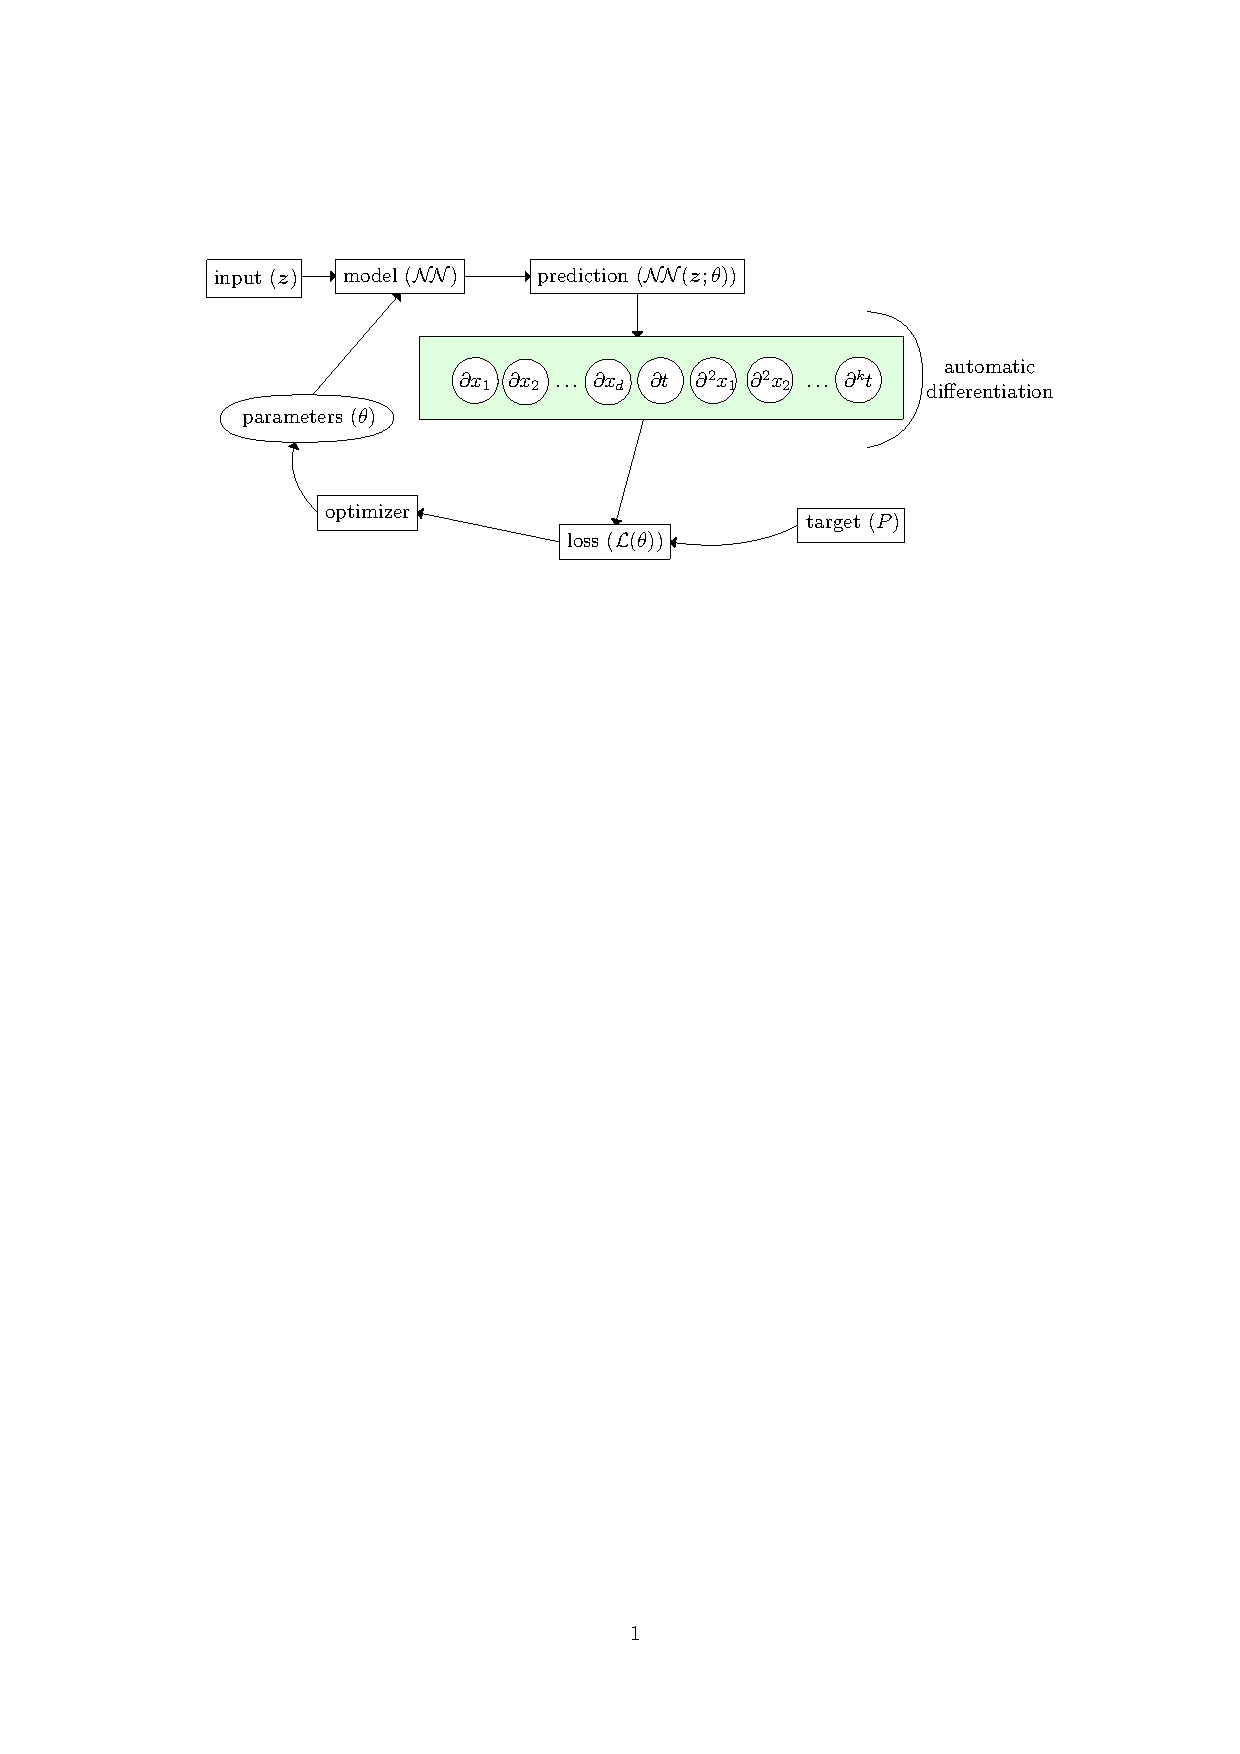
\includegraphics[width=\textwidth, clip=true, trim={3cm 20cm 3cm 4cm}]{imagenes/autodiffgraph.pdf}}
  \caption{Components of a PINN during the training phase, where we solve \eqref{loss-fun-pinn}.
  }\label{fig:autodiffgraph}
\end{figure}

\section{RBF/Polynomial approximation}

\chapter{Interpolation}

During this section, we shall present some key definitions and results
following the discussion proposed by Fasshauer \cite{fasshauer2007meshfree}.

\begin{problem}
({\tmstrong{Scattered data interpolation}}) Given $\{ (\tmmathbf{x}_j, y_j)
  \}_{j = 1}^N \subset \mathbb{R}^d \times \mathbb{R}$, find a function
$\mathcal{P}$ such that $\mathcal{P} (\tmmathbf{x}_j) = y_j$ for all $j = 1,
  \ldots, N$.\label{interpolationproblemstatement}
\end{problem}

One strategy for tackling this problem is by further assuming $\mathcal{P}$ is
a linear combination of a family of continuous basis functions $\{ \phi_j
  \}_{j = 1}^N$ on a compact metric space $\mathcal{X}$, i.e.,
\begin{equation}
  \mathcal{P} (\tmmathbf{x}) = \sum_{k = 1}^N \lambda_k \phi_k (\tmmathbf{x})
  . \label{eqn-p-is-a-linear-combination}
\end{equation}
\begin{definition}
  A function $\tmmathbf{x} \mapsto \mathcal{P} (\tmmathbf{x})$ with
  $\mathcal{P}$ as in \eqref{eqn-p-is-a-linear-combination} is called a
    {\tmstrong{generalized polynomial}}.
\end{definition}

We would then be tasked to find $\lambda_1, \ldots, \lambda_N \in \mathbb{R}$
such that
\[ \sum_{k = 1}^N \lambda_k \phi_k (\tmmathbf{x}_1) =\tmmathbf{y}_1, \sum_{k =
    1}^N \lambda_k \phi_k (\tmmathbf{x}_2) =\tmmathbf{y}_2, \ldots, \sum_{k =
    1}^N \lambda_k \phi_k (\tmmathbf{x}_N) =\tmmathbf{y}_N . \]
Note the scalar products
\[ \left\{\begin{array}{cll}
    \left(\begin{array}{ccc}
              \lambda_1 & \cdots & \lambda_N
            \end{array}\right) \left(\begin{array}{ccc}
                                     \phi_1 (\tmmathbf{x}_1) & \cdots & \phi_N (\tmmathbf{x}_1)
                                   \end{array}\right)^{\top} & = & \tmmathbf{y}_1 \\
    \left(\begin{array}{ccc}
              \lambda_1 & \cdots & \lambda_N
            \end{array}\right) \left(\begin{array}{ccc}
                                     \phi_1 (\tmmathbf{x}_2) & \cdots & \phi_N (\tmmathbf{x}_2)
                                   \end{array}\right)^{\top} & = & \tmmathbf{y}_2 \\
    \vdots                                                      &   &                         \\
    \left(\begin{array}{ccc}
              \lambda_1 & \cdots & \lambda_N
            \end{array}\right) \left(\begin{array}{ccc}
                                     \phi_1 (\tmmathbf{x}_N) & \cdots & \phi_N (\tmmathbf{x}_N)
                                   \end{array}\right)^{\top} & = & \tmmathbf{y}_N
  \end{array}\right. . \]
This system induces the system of linear equations
\begin{equation}
  \left(\begin{array}{cccc}
      \phi_1 (\tmmathbf{x}_1) & \phi_2 (\tmmathbf{x}_1) & \cdots & \phi_N
      (\tmmathbf{x}_1)                                                    \\
      \phi_1 (\tmmathbf{x}_2) & \phi_2 (\tmmathbf{x}_2) & \cdots & \phi_N
      (\tmmathbf{x}_2)                                                    \\
      \vdots                  & \vdots                  &        & \vdots \\
      \phi_1 (\tmmathbf{x}_N) & \phi_2 (\tmmathbf{x}_N) & \cdots & \phi_N
      (\tmmathbf{x}_N)
    \end{array}\right) \left(\begin{array}{c}
      \lambda_1 \\
      \lambda_2 \\
      \vdots    \\
      \lambda_N
    \end{array}\right) = \left(\begin{array}{c}
      \tmmathbf{y}_1 \\
      \tmmathbf{y}_2 \\
      \vdots         \\
      \tmmathbf{y}_N
    \end{array}\right) \label{linear-system-equations-generalized-poly}
\end{equation}
which follows the familiar form
\begin{equation}
  A \underline{\lambda} = y \label{matrixexpression-interpolationprob} .
\end{equation}
\begin{definition}
  The matrix $A$ in formulation \eqref{matrixexpression-interpolationprob} is said to
  be the {\tmstrong{interpolation matrix}}.
\end{definition}

\begin{definition}
  Under the hypotheses of Problem \ref{interpolationproblemstatement}, and
  further assuming \eqref{eqn-p-is-a-linear-combination}, we will say that the problem is
    {\tmstrong{well-posed}} (i.e., there is a unique solution to the problem) if
  and only if $A$ is non-singular.
\end{definition}


We shall now present some broadly stated results that can be found in Cheney \cite{cheney1966introduction}:

\begin{theorem}
  (Existence of the best approximations in a metric space). Let $K$ denote a
  compact set in a metric space $\mathcal{X}$. Then, for every $p \in
    \mathcal{X}$ there corresponds
  \[ k^{\ast} = \arg \min_{k \in K} d (p, k), \]
  where $d$ is the distance on $\mathcal{X}$.
\end{theorem}

This statement may (mis)lead us into only regarding $p$ and $k$ as points in
a Euclidean space. On the contrary, recall that any two functions $f, g \in
  L^p (\Omega)$ with $\Omega$ a bounded set, are also governed by the previous
theorem by setting $d (f, g) = \| f - g \|_{L^p}$, where $\| \cdot \|_{L^p}$
denotes the $L^p -$norm. Profound yet manageable results on generalized
polynomials can be given by further requesting them to satisfy the Haar
condition.

\begin{definition}
  The family of functions $\{ \phi_j \}_{j = 1}^N$ of Problem
  \ref{interpolationproblemstatement} is said to satisfy the {\tmstrong{Haar
        condition}} if every set of $N$ vectors of the form $\hat{\tmmathbf{x}} =
    (\phi_1 (\tmmathbf{x}), \phi_2 (\tmmathbf{x}), \ldots, \phi_N
    (\tmmathbf{x}))$ is linearly independent. The finite-dimensional linear function space induced by $\{ \phi_j \}_{j = 1}^N$ is said to be a {\tmstrong{Haar
        space}}.
\end{definition}

The property of linear independence can alternatively be expressed by
considering any $N$ distinct points  \{$\tmmathbf{x}_1, \ldots,
  \tmmathbf{x}_N$\}  and checking that
\[ \text{det}  [\hat{\tmmathbf{x}}_1, \hat{\tmmathbf{x}}_2, \ldots,
    \hat{\tmmathbf{x}}_n] = \left|\begin{array}{cccc}
    \phi_1 (\tmmathbf{x}_1) & \phi_2 (\tmmathbf{x}_1) & \cdots & \phi_N
    (\tmmathbf{x}_1)                                                    \\
    \phi_1 (\tmmathbf{x}_2) & \phi_2 (\tmmathbf{x}_2) & \cdots & \phi_N
    (\tmmathbf{x}_2)                                                    \\
    \vdots                  & \vdots                  &        & \vdots \\
    \phi_1 (\tmmathbf{x}_N) & \phi_2 (\tmmathbf{x}_N) & \cdots & \phi_N
    (\tmmathbf{x}_N)
  \end{array}\right| \neq 0. \]
Provided the Haar condition is satisfied,
\eqref{linear-system-equations-generalized-poly} features a unique solution.

In the case $\{ x_1, \ldots, x_N \} \subset \mathbb{R}$, we know that problem
\ref{interpolationproblemstatement} can be solved considering a polynomial of
degree $N - 1$. One could (mistakenly) venture that a similar result would be devolved for
higher dimensions, considering multivariate polynomials of degree $N-1$.

\begin{theorem}\label{thm-haar-spaces-polynomials}
  Let $\Omega \subset \mathbb{R}^d, d \geq 2$. If $\Omega$ contains an
  interior point, then there exist no Haar spaces of continuous functions except for one-dimensional ones.
\end{theorem}

\begin{proof}
  Consider any distinct $\{ \tmmathbf{x}_1, \ldots, \tmmathbf{x}_N \} \subset
    \mathbb{R}^d$ and construct the matrix $A$ as in
  \eqref{matrixexpression-interpolationprob}. If the Haar condition were
  satisfied, then $\text{det} (A) \neq 0$. Now, note that $$\text{det}
    [\hat{\tmmathbf{x}}_1, \hat{\tmmathbf{x}}_2, \ldots, \hat{\tmmathbf{x}}_n] =
    - \text{det} [\hat{\tmmathbf{x}}_2, \hat{\tmmathbf{x}}_1, \ldots,
      \hat{\tmmathbf{x}}_n].$$ Because $\Omega$ contains an interior point, we may
  consider a closed path that connects exclusively $\tmmathbf{x}_1$ and
  $\tmmathbf{x}_2$\footnote{Indeed, this path would be of measure zero in
    $\Omega$. Consequently, it can be defined to not contain $\tmmathbf{x}_3,
      \tmmathbf{x}_4, \ldots, \tmmathbf{x}_N$ along its traversal.}. We now
  continuously exchange the positions of $\tmmathbf{x}_1$ and
  $\tmmathbf{x}_2$, whereby the sign of the determinant has changed
  at its conclusion. This exchange is a continuous function of $\tmmathbf{x}_1$
  and $\tmmathbf{x}_2$. Consequently, the determinant has been zero along some
  point of the path, which is a contradiction. Note that, because the path is
  closed, the exchange function can be chosen so that we do not have
  $\tmmathbf{x}_1 = \tmmathbf{x}_2$ at any point of the exchange.
\end{proof}

Consequently, if we want to solve interpolate for a well-posed problem, it will not suffice to solve for a pre-fixed generalized polynomial. We can proceed instead by establishing a ``dependence of the basis with respect to the input data''. One possible path for doing so is considering \textbf{Radial Basis Functions}.

\begin{definition}\label{radialfunctions}
  A function $\phi : \mathbb{R}^d \rightarrow \mathbb{R}$ is said to be
    {\tmstrong{radial}} if there exists some univariate function $\varphi$ such
  that $\phi (\tmmathbf{x}) = \varphi (\| \tmmathbf{x} \|)$, where $\| \cdot
    \|$ is a norm on $\mathbb{R}^d$.
\end{definition}

The {\tmem{radial}} adjective stems from the fact that
\[ \| \tmmathbf{x}_1 \| = \| \tmmathbf{x}_2 \| \Rightarrow \varphi (\|
  \tmmathbf{x}_1 \|) = \varphi (\| \tmmathbf{x}_2 \|) \Rightarrow \phi
  (\tmmathbf{x}_1) = \phi (\tmmathbf{x}_2), \quad \forall \tmmathbf{x}_1,
  \tmmathbf{x}_2 \in \mathbb{R}^d . \]
That is, $\phi$ is radially symmetric about its center.

Furthermore, characterization in definition \ref{radialfunctions} implies that the scattered data interpolation problem can be expressed in terms of univariate functions of a given norm.
This implies that \eqref{eqn-p-is-a-linear-combination} is further refined into an
expression of the form
\begin{equation}
  \mathcal{P} (\tmmathbf{x}) = \sum_{k = 1}^N \lambda_k \varphi (\|
  \tmmathbf{x}-\tmmathbf{x}_k \|_2), \quad \tmmathbf{x} \in \mathbb{R}^d,
  \label{eqn-p-is-a-linear-combination-of-rbfs}
\end{equation}
where $\tmmathbf{x}_k$ are usually referred to as \textbf{centers}. This ultimately reshapes \eqref{linear-system-equations-generalized-poly} into
\begin{equation}
  \left(\begin{array}{cccc}
      \varphi (\| \tmmathbf{x}_1 -\tmmathbf{x}_1 \|_2) & \varphi (\|
      \tmmathbf{x}_1 -\tmmathbf{x}_2 \|_2)             & \ldots      & \varphi (\| \tmmathbf{x}_1
      -\tmmathbf{x}_N \|_2)                                                                                \\
      \varphi (\| \tmmathbf{x}_2 -\tmmathbf{x}_1 \|_2) & \varphi (\|
      \tmmathbf{x}_2 -\tmmathbf{x}_2 \|_2)             & \ldots      & \varphi (\| \tmmathbf{x}_2
      -\tmmathbf{x}_2 \|_2)                                                                                \\
      \vdots                                           & \vdots      & \ddots                     & \vdots \\
      \varphi (\| \tmmathbf{x}_N -\tmmathbf{x}_1 \|_2) & \varphi (\|
      \tmmathbf{x}_N -\tmmathbf{x}_2 \|_2)             & \ldots      & \varphi (\| \tmmathbf{x}_N
      -\tmmathbf{x}_N \|_2)
    \end{array}\right) \left(\begin{array}{c}
      \lambda_1 \\
      \lambda_2 \\
      \vdots    \\
      \lambda_N
    \end{array}\right) = \left(\begin{array}{c}
      f (\tmmathbf{x}_1) \\
      f (\tmmathbf{x}_2) \\
      \vdots             \\
      f (\tmmathbf{x}_N)
    \end{array}\right).
  \label{eqn-linear-system-equations-rbf}
\end{equation}

In the case where the problem is overdetermined (that is, we consider more data
points than centers), the matrix $A$ is no longer square (say, now $A \in
  \mathbb{R}^{m \times n}$). In such case, we come up against a linear optimization
problem where we try to find some suitable set of parameters, say $\lambda$,
such that $\| A \lambda - f \|_2$ is minimum. The solution to this problem is
then given by all $\hat{\lambda} \in \mathbb{R}^n$ satisfying the normal
equations,
\begin{equation}
  (A^{\top} A) \hat{\lambda} = A^{\top} f \label{eqn-normal-equation} .
\end{equation}
Indeed, note that
\[ \| A \lambda - f \|_2^2 = (A \lambda - f)^{\top} (A \lambda - f) =
  \lambda^{\top} (A^{\top} A \lambda - 2 A^{\top} f) + f^{\top} f. \]
Now, we differentiate with respect to the $i -$th entry of $\lambda$, which
yields
\[ e_i^{\top} (A^{\top} A \lambda - 2 A^{\top} f) + \lambda^{\top} (A^{\top} A
  e_i) = 2 e_i^{\top} (A^{\top} A \lambda - A^{\top} f), \]
where $e_i$ denotes the vector who is identically zero except for its $i -$th
entry, with value $1$. Finally,
\[ 2 e_i^{\top} (A^{\top} A \lambda - A^{\top} f) = 0 \Leftrightarrow
  A^{\top} A \lambda - A^{\top} f = 0 \Leftrightarrow (A^{\top} A) \lambda =
  A^{\top} f, \]
which is exactly \eqref{eqn-normal-equation}. Note that $A^{\top} A \in
  \mathbb{R}^{n \times n}$, which may or may not be invertible. Regardless, we
can find $\hat{\lambda}$ taking the Moore-Penrose pseudo-inverse of $A$,
presented in the following.

\begin{definition}
  Let $A \in \mathbb{R}^{m \times n}$. Then, we define the
    {\tmstrong{Moore-Penrose pseudo-inverse}}, $A^{\dag}$, as
  \[ A^{\dag} = \lim_{\varepsilon \rightarrow 0} (A^{\top} A + \varepsilon
    I_n)^{- 1} A^{\top} . \]
\end{definition}

Now, observe that \eqref{eqn-normal-equation} can be rewritten as
\[ \lim_{\varepsilon \rightarrow 0} (A^{\top} A + \varepsilon I_n)
  \hat{\lambda} = A^{\top} f. \]
Multiplying by $(A^{\top} A + \varepsilon I_n)^{- 1}$ on both sides of the
equality, we have
\[ \lim_{\varepsilon \rightarrow 0} (A^{\top} A + \varepsilon I_n)^{- 1}
  (A^{\top} A + \varepsilon I_n) \hat{\lambda} = \lim_{\varepsilon
    \rightarrow 0} (A^{\top} A + \varepsilon I_n)^{- 1} A^{\top} f \Rightarrow
  \hat{\lambda} = A^{\dag} f. \]
Indeed, even if the matrix for the overdetermined problem is not invertible
(that is, we are not using any of the soon-to-be-presented radial basis
functions), we can still find minimizers of the scattered interpolation
problem in the least squares sense.


\begin{definition}
  A real symmetric matrix $A \in \mathbb{R}^{n \times n}$ is called
    {\tmstrong{positive semi-definite}} if $\tmmathbf{x}^{\top} A\tmmathbf{x}
    \geq 0$ for all $\tmmathbf{x} \in \mathbb{R}^n$. In the case the equality
  holds if and only if $\tmmathbf{x}= 0$, we say that $A$ is
    {\tmstrong{positive definite}}.
\end{definition}

Note that if $A$ is positive semi-definite, all its eigenvalues are positive.
Indeed, if $x$ is an eigenvector of $A$ associated to an eigenvalue $\lambda$,
we have $0 < x^{\top} A x = \lambda x^{\top} x$, and because $x^{\top} x$ is
the Euclidean inner product involving non-zero vectors, we conclude $\lambda >
  0$. This implies that a positive definite matrix is non-singular.

It would be ideal for our purposes to construct positive-definite
interpolation matrices. That way, $\eqref{eqn-linear-system-equations-rbf}$ would
be well-posed.

\begin{definition}\label{def-positive-definite-functions}
  A function $\phi : \mathbb{R}^d \rightarrow \mathbb{C}$ is called
    {\tmstrong{positive definite}} on $\mathbb{R}^d$ if
  \begin{equation}
    \sum_{j = 1}^N \sum_{k = 1}^N c_j \overline{c_k} \phi (\tmmathbf{x}_j
    -\tmmathbf{x}_k) \geq 0 \label{positivedefinitefunctioncomplexdefinition}
  \end{equation}
  for any pairwise different points $\tmmathbf{x}_1, \ldots, \tmmathbf{x}_N
    \in \mathbb{R}^d$ and $\tmmathbf{c}= (c_1, \ldots, c_N)^{\top} \in
    \mathbb{C}^N$. In the case the equality holds if an only if $\tmmathbf{c}=
    0$, we shall say that $\phi$ is {\tmstrong{strictly positive definite}}.
\end{definition}

\begin{example}
  \label{funexampleutil}For a fixed $\tmmathbf{y} \in \mathbb{R}^d$, define
  $\phi (\tmmathbf{x}) = e^{i\tmmathbf{x} \cdot \tmmathbf{y}}$, where
  $\tmmathbf{x} \cdot \tmmathbf{y}$ denotes the inner product. Then, for any
  $\tmmathbf{c}= (c_1, \ldots, c_N)^{\top} \in \mathbb{C}^N$, we have
  \[ \begin{array}{ccc}
      \sum_{j = 1}^N \sum_{k = 1}^N c_j \overline{c_k} \phi (\tmmathbf{x}_j
      -\tmmathbf{x}_k) & = & \sum_{j = 1}^N \sum_{k = 1}^N c_j \overline{c_k}
      e^{i (\tmmathbf{x}_j -\tmmathbf{x}_k) \cdot \tmmathbf{y}}                        \\
                       & = & \sum_{j = 1}^N \sum_{k = 1}^N c_j \overline{c_k}
      e^{i\tmmathbf{x}_j \cdot \tmmathbf{y}- i\tmmathbf{x}_k \cdot
      \tmmathbf{y}}                                                                    \\
                       & = & \sum_{j = 1}^N c_j e^{i\tmmathbf{x}_j \cdot \tmmathbf{y}}
      \sum_{k = 1}^N \overline{c_k} e^{- i\tmmathbf{x}_k \cdot \tmmathbf{y}}
      .
    \end{array} \]
  For each $j = 1, \ldots, N$, we have that the conjugate of $c_j
    e^{i\tmmathbf{x}_j \cdot \tmmathbf{y}}$ is $\overline{c_k} e^{-
        i\tmmathbf{x}_k \cdot \tmmathbf{y}}$. Therefore,
  \begin{equation}
    \sum_{j = 1}^N \sum_{k = 1}^N c_j \overline{c_k} \phi (\tmmathbf{x}_j
    -\tmmathbf{x}_k) = \left| \sum_{j = 1}^N c_j e^{i\tmmathbf{x}_j \cdot
        \tmmathbf{y}} \right|^2 \geq 0 \label{positivedefinitepropertyasmodulus}
  \end{equation}
  and $\phi$ is positive definite.
\end{example}

\begin{theorem}
  Let $\phi_1, \ldots, \phi_N$ be positive definite functions on
  $\mathbb{R}^d$ and $c_j \geq 0$ for $j = 1, \ldots, N$. We consider their
  finite linear combination,
  \begin{equation}
    \phi (\tmmathbf{x}) = \sum_{j = 1}^N c_j \phi_j (\tmmathbf{x}), \quad
    \tmmathbf{x} \in \mathbb{R}^d . \label{linearcombinationofpsdf}
  \end{equation}
  Then, we have that
  \begin{enumerate}
    \item $\phi$ is positive definite. Moreover, it is enough that one of the
          $\phi_j$'s is strictly positive definite (with $c_j > 0$) for $\phi$ to be
          strictly positive definite.

    \item $\phi (\tmmathbf{0}) \geq 0$.

    \item \label{propevennes}$\phi (-\tmmathbf{x}) = \overline{\phi
              (\tmmathbf{x})}$.

    \item $| \phi (\tmmathbf{x}) | \leq \phi (\tmmathbf{0})$. In fact, any
          positive definite function is bounded.

    \item $\phi$ positive definite with $\phi (\tmmathbf{0}) = 0 \Rightarrow
            \phi \equiv 0$.

    \item The product of (strictly) positive definite functions is (strictly)
          positive definite functions.
  \end{enumerate}
\end{theorem}

Note that in the case that $\phi$ is a real function, property
\eqref{propevennes} implies that $\phi$ is even. In fact, this allows us to
characterize positive-definite real-valued continuous functions.

\begin{theorem}
  A real-valued continuous function $\phi$ is {\tmstrong{positive definite}}
  on $\mathbb{R}^d$ if and only if it is even and
  \[ \sum_{j = 1}^N \sum_{k = 1}^N c_j c_k \phi (\tmmathbf{x}_j
    -\tmmathbf{x}_k) \geq 0 \]
  for any pairwise different points $\tmmathbf{x}_1, \ldots, \tmmathbf{x}_N
    \in \mathbb{R}^d$ and $\tmmathbf{c}= (c_1, \ldots, c_N)^{\top} \in
    \mathbb{C}^N$. In the case the equality holds if and only if $\tmmathbf{c}=
    0$, $\phi$ is {\tmstrong{strictly positive definite}}.
\end{theorem}

\begin{theorem}\label{tm-bochner}
  ({\tmstrong{Bochner}}) A continuous function $\phi : \mathbb{R}^d
    \rightarrow \mathbb{C}$ is positive definite on $\mathbb{R}^d$ if and only
  if it is the Fourier transform of a finite Borel measure $\mu$
  on $\mathbb{R}^d$, that is, if
  \begin{equation}
    \phi (\tmmathbf{x}) = \frac{1}{\sqrt{(2 \pi)^d}} \int_{\mathbb{R}^d} e^{-
        i\tmmathbf{x} \cdot \tmmathbf{y}} d \mu (\tmmathbf{y}), \quad \tmmathbf{x}
    \in \mathbb{R}^d . \label{characterizationphitransform}
  \end{equation}
\end{theorem}

From a strategic point of view, we actually only need to prove the direction of the characterization yielding that $\phi$ is positive definite. This is the case where we assume \eqref{characterizationphitransform}. Moreover, recall that a Borel measure is one whose domain of application is the $\sigma-$algebra of Borel sets, that is, the smallest $\sigma-$algebra containing all open sets of a given topological space, $(X,\tau)$.

\begin{proof}
  Applying definition \eqref{positivedefinitefunctioncomplexdefinition}, we
  have that
  \[ \begin{array}{ccc}
      \sum_{j = 1}^N \sum_{k = 1}^N c_j \overline{c_k} \phi (\tmmathbf{x}_j
      -\tmmathbf{x}_k)                                       &
      \xequal[\text{\eqref{characterizationphitransform}}]{} &
      \frac{1}{\sqrt{(2 \pi)^d}} \sum_{j = 1}^N \sum_{k = 1}^N \left[ c_j
        \overline{c_k} \int_{\mathbb{R}^d} e^{- i (\tmmathbf{x}_j
      -\tmmathbf{x}_k) \cdot \tmmathbf{y}} d \mu (\tmmathbf{y}) \right]                                                                                 \\
      \text{(linearity of integral)}                         & =                                                           & \frac{1}{\sqrt{(2 \pi)^d}}
      \int_{\mathbb{R}^d} \left[ \sum_{j = 1}^N c_j e^{- i\tmmathbf{x}_j
            \cdot \tmmathbf{y}} \sum_{k = 1}^N \overline{c_k} e^{i\tmmathbf{x}_k
      \cdot \tmmathbf{y}} \right] d \mu (\tmmathbf{y})                                                                                                  \\
                                                             & \xequal[\text{\eqref{positivedefinitepropertyasmodulus}}]{} &
      \frac{1}{\sqrt{(2 \pi)^d}} \int_{\mathbb{R}^d} \left| \sum_{j = 1}^N
      c_j e^{- i\tmmathbf{x}_j \cdot \tmmathbf{y}} \right|^2 d \mu
      (\tmmathbf{y})                                                                                                                                    \\
                                                             & \geq                                                        & 0.
    \end{array} \]
  The inequality holds due to the non-negativity of the Borel measure.
\end{proof}

A direct consequence of this Theorem is that the function proposed in Example
\ref{funexampleutil} deserves special interest, for any other positive
definite function can be defined in terms of (infinite) linear combinations of
it, which is a more surprising result that linear combinations of the form
\eqref{linearcombinationofpsdf} resulting in (some) positive definite
function.

Even though Theorem \ref{tm-bochner} highlights the relevance
of the Gaussian function, its application is not straightforward
for deciding the positive definiteness of a function.
We shall garner more specialized tools in the following.
To this end, we first take a step back and define some key building blocks: we
start out following the presentation in {\cite{titchmarsh1939theory}}:

\begin{definition}
  Let $\varnothing = \Omega \subset \mathbb{C}$ be an open set. A function $g
    : \Omega \rightarrow \mathbb{C}$ is said to be {\tmstrong{analytic}} in $a
    \in \Omega$ if there is a power series centered in $a$ with radius $R > 0$
  such that
  \begin{equation}
    g (z) = \sum_{n = 0}^{\infty} a_n (z - a)^n
    \label{analyticasseriedepotencia}, \text{ with } | z - a | < \rho .
  \end{equation}
  That is, $g$ coincides with a power series in a neighborhood of $a$.
  Moreover, $g$ is said to be {\tmstrong{analytic}} in $\Omega$ if it is
  analytic for every $a \in \Omega$.
\end{definition}

Note that $g (a) = 0 \Rightarrow a_0 = 0$. In fact, some other coefficients
$a_1, a_2, \ldots$ may be zero. Furthermore, if $a_n = 0$ for all $n < m \in
  \mathbb{N}$ and $a_m \neq 0$, we say $g$ to have a {\tmstrong{zero of the}} $m
  -${\tmstrong{th order}}. In such case, we also have
\[ g (a) = g' (a) = \cdots = g^{m - 1} (a) = 0, \text{ and } g^m (a) \neq 0,
\]
which is clear due to \eqref{analyticasseriedepotencia}.

\begin{theorem}
  \label{theorem-titschmarch}Let $z \mapsto g (z)$ be an analytic function in
  a region $S$, and let $s_1, s_2, \ldots, s_n, \ldots$ be a set of points
  whose point of accumulation is some $s \in S$. If $g (s_i) = 0$ for every $i
    \in \mathbb{N}$, then $g (z) = 0$ for all $z \in S$.
\end{theorem}

\begin{proof}
  Because $g$ is analytic in a region $S$, identity
  \eqref{analyticasseriedepotencia} applies. Without loss of generality, we
  assume that our point of accumulation $s = a = 0$, which implies $g (z) =
    \sum_{n = 0}^{\infty} a_n z^n$ for some radius $R > 0$. To show that $g (z)
    = 0$ for all $z \in S$, we only need to show that every coefficient in
  \eqref{analyticasseriedepotencia} is zero. If that were not the case, we
  would have
  \[ g (z) = \sum_{n = k}^{\infty} a_n z^n = z^k (a_k + a_{k + 1} z + \cdots),
    \text{ for all } 0 < \rho < R. \]
  In such case, the series $\sum_{n = k}^{\infty} a_n \rho^n$ is convergent,
  which implies that each $a_n \rho^n$ is bounded, so $| a_n | \rho^n \leq K$
  for some $K$. Hence,
  \[ | g (z) | \geq | z |^k \left( | a_k | - \frac{K | z |}{\rho^{k + 1}} -
    \frac{K | z |^2}{\rho^{k + 2}} - \cdots \right) = | z |^k \left( | a_k |
    - \frac{K | z |}{\rho^k (\rho - | z |)} \right) . \]
  Because $| a_k |$ is fixed, we can make the right-hand side of the
  inequality strictly positive by taking $| z |$ sufficiently small (but not
  equal to zero). This is a contradiction with the assumption that $s = 0$ is
  an accumulation point: actually, every coefficient in $\sum_{n = 0}^{\infty}
    a_n z^n$ needs to vanish, which allows us to conclude $g (z) = 0$ for every
  $z \in S$.
\end{proof}

The following two lemmas are as formulated in {\cite{cheneylight2009course}}.

\begin{lemma}
  \label{lemma-linearly-independent-set-featuring-accumulation}Let $\{
    \lambda_j \}_{i = 1}^N$ be a set of distinct complex numbers. Then, $\{
    e^{\lambda_j z} \}_{i = 1}^N$ is a linearly independent set on any domain in
  $\mathbb{C}$ featuring a point of accumulation.
\end{lemma}

\begin{proof}
  We show the result by induction, first noting that $z \mapsto e^{\lambda_1
        z}$ is nonzero for any $z \in \mathbb{C}$. Assuming the result holds for
  some $N \in \mathbb{N}$, we define $g (z) = \sum_{j = 1}^{N + 1} c_j e^{-
        \lambda_j z}$ and assume that $g (z) = 0$ for some $z \in S \subset
    \mathbb{C}$, where $S$ has a point of accumulation. Because $g$ is an entire
  function, it follows that $g (z) = 0$ for all $z \in \mathbb{C}$. Now, we
  define
  \[ F (z) = \frac{d}{d z} (e^{- \lambda_{N + 1} z} g (z)) = \frac{d}{d z}
    \left( \sum_{j = 1}^{N + 1} c_j e^{(\lambda_j - \lambda_{N + 1}) z}
    \right) = \]
  \[ = \frac{d}{d z} \left( \sum_{j = 1}^N c_j e^{(\lambda_j - \lambda_{N +
            1}) z} + c_{N + 1} \right) = \sum_{j = 1}^N c_j (\lambda_j - \lambda_{N +
      1}) e^{(\lambda_j - \lambda_{N + 1}) z} . \]
  Because $g (z) = 0$ for all $z \in \mathbb{C}$, we have that $F \equiv 0$
  too. Applying the induction hypothesis to the set of $\{ \lambda_j -
    \lambda_{N + 1} \}_{j = 1}^N$ distinct complex numbers, we obtain that $\{
    e^{(\lambda_j - \lambda_{N + 1}) z} \}_{j = 1}^N$ is a linearly independent
  set on $S$. Therefore, $c_j (\lambda_j - \lambda_{N + 1}) = 0$ for all $j =
    1, \ldots, N$, which ultimately implies $c_j = 0$ because we assumed
  $\lambda_j \neq \lambda_{N + 1}$. Hence, $g (z) = c_{N + 1} e^{- \lambda_{N
          + 1} z} = 0$ for all $z \in \mathbb{C}$, which yields $c_{N + 1} = 0$ too.
  Consequently, $\{ e^{\lambda_j z} \}_{i = 1}^{N + 1}$ is linearly
  independent on $S$ as well.
\end{proof}

\begin{lemma}
  \label{lemma-no-accumulation-point}Let $\{ \lambda_j \}_{i = 1}^N$ be a set
  of distinct complex numbers and define the complex function $g (z) = \sum_{j
      = 1}^N c_j e^{\lambda_j z}$, assuming that some $c_1, c_2, \ldots, c_N$ is
  nonzero. Then, the set of zeros of $g$ features no point of accumulation.
\end{lemma}

\begin{proof}
  Lemma \ref{lemma-linearly-independent-set-featuring-accumulation} implies
  that $\{ e^{\lambda_j z} \}_{i = 1}^N$ is a linearly independent set on any
  domain in $\mathbb{C}$ featuring a point of accumulation, which implies $g
    \neq 0$. Because $g$ is an entire function, by definition it is analytic at
  every $z \in \mathbb{C}$. The contrapositive of Theorem
  \ref{theorem-titschmarch} implies that the set of zeros of $g$ has no
  accumulation points.
\end{proof}

\begin{definition}
  Let $X$ be a topological space and $\mu$ be a Borel measure.
  The {\tmstrong{carrier }}of $\mu$ is defined as
  \[ X\backslash \bigcup \left\{ \mathcal{O}: \mathcal{O} \text{ is open and }
    \mu (\mathcal{O}) = 0 \right\} . \]
\end{definition}

\begin{theorem}
  Let $\mu$ be a finite Borel measure on $\mathbb{R}^d$ whose
  carrier is a set of nonzero Lebesgue measure. Then, the Fourier transform of
  $\mu$ is strictly positive definite on $\mathbb{R}^d$.
\end{theorem}

\begin{proof}
  Let $\hat{\mu}$ denote the Fourier transform of $\mu$. By hypothesis,
  we have
  \[ \sum_{j = 1}^N \sum_{k = 1}^N c_j \overline{c_k} \hat{\mu}
    (\tmmathbf{x}_j -\tmmathbf{x}_k) = \frac{1}{\sqrt{(2 \pi)^d}} \sum_{j =
      1}^N \sum_{k = 1}^N c_j \overline{c_k}  \left[ \int_{\mathbb{R}^d} e^{- i
          (\tmmathbf{x}_j -\tmmathbf{x}_k) \cdot \tmmathbf{y}} d \mu (\tmmathbf{y})
      \right] . \]
  Applying the linearity of the integral on the right-hand side, we have
  \[ \sum_{j = 1}^N \sum_{k = 1}^N c_j \overline{c_k} \hat{\mu}
    (\tmmathbf{x}_j -\tmmathbf{x}_k) = \frac{1}{\sqrt{(2 \pi)^d}}
    \int_{\mathbb{R}^d} \left[ \sum_{j = 1}^N c_j e^{- i\tmmathbf{x}_j \cdot
          \tmmathbf{y}} \sum_{k = 1}^N \overline{c_k} e^{i\tmmathbf{x}_k \cdot
          \tmmathbf{y}} \right] d \mu (\tmmathbf{y}) \]
  The integrand on the right-hand side can be rearranged using
  \eqref{positivedefinitepropertyasmodulus}, to yield
  \begin{equation}
    \sum_{j = 1}^N \sum_{k = 1}^N c_j \overline{c_k} \hat{\mu} (\tmmathbf{x}_j
    -\tmmathbf{x}_k) = \int_{\mathbb{R}^d} \left| \sum_{j = 1}^N c_j e^{-
        i\tmmathbf{x}_j \cdot \tmmathbf{y}} \right|^2 d \mu (\tmmathbf{y}) \geq 0,
    \label{non-strict-inequality-measure-borel}
  \end{equation}
  due again to the non-negativity property of a measure. This is only enough to
  show positive definiteness. In order to show the strict positive
  definiteness, we further work on the integrand. To this end, define the
  function
  \[ g (\tmmathbf{y}) = \sum_{j = 1}^N c_j e^{- i\tmmathbf{x}_j \cdot
        \tmmathbf{y}} \]
  and assume that all points $\tmmathbf{x}_j$ are distinct, $j = 1, \ldots,
    N$. Furthermore, assume that $\tmmathbf{c} \neq 0$. As per Lemma
  \ref{lemma-linearly-independent-set-featuring-accumulation}, the set of
  functions $\{ e^{- i\tmmathbf{x}_j \cdot \tmmathbf{y}} \}_{j = 1}^N$ is
  linearly independent, which implies $g \neq 0$.

  Now, consider the zero set of $g$, namely $\{ \tmmathbf{x} \in \mathbb{R}^d
    : g (\tmmathbf{x}) = 0 \}$. Due to Lemma \ref{lemma-no-accumulation-point},
  none of the elements of this set is an accumulation point, which implies
  that its elements are isolated and that the Lebesgue measure of the set is
  zero. The only way to have \eqref{non-strict-inequality-measure-borel} be an
  equality would be if the carrier of $\mu$ were to have zero Lebesgue
  measure, which is assumed to not happen by hypothesis.
\end{proof}

\begin{corollary}\label{cor-fourier-strictly-positive-def}
  Let $g$ be a continuous non-negative function in $L^1 (\mathbb{R}^d)$ that
  is not identically zero. Then, the Fourier transform of $g$ is strictly
  positive definite on $\mathbb{R}^d$.
\end{corollary}

\begin{proof}
  This result is a particular case of the previous one: define the measure
  $\mu$ for any Borel set $B \subset \mathbb{R}^d$ as
  \[ \mu (B) = \int_B g (\tmmathbf{x}) d\tmmathbf{x}= \int_B | g
    (\tmmathbf{x}) | d\tmmathbf{x}, \]
  which is bounded because $g \in L^1 (\mathbb{R}^d)$. Furthermore, the
  non-negativity of $g$ implies that the previous integral identity holds.

  The carrier of $\mu$ is, by definition, the support of $g$. Because $g$ is
  assumed to not identically equal to zero, the continuity of $g$ implies that
  its support has positive Lebesgue measure. Consequently, the previous
  Theorem implies that the Fourier transform of $g$ is strictly positive
  definite.
\end{proof}

The discussion ranging from Definition \ref{def-positive-definite-functions}
up until this point has been on positive definite functions, of the form $\phi
  : \mathbb{R}^d \rightarrow \mathbb{C}$. If $\phi$ is radial, Definition
\ref{radialfunctions} establishes $\phi (\tmmathbf{x}) = \varphi (\|
  \tmmathbf{x} \|)$. A direct consequence of this is

\begin{lemma}
  If $\phi$ is a (strictly) positive definite and radial function on
  $\mathbb{R}^d$, then $\phi$ is also (strictly) positive definite and radial
  on $\mathbb{R}^{\delta}$, for any $\delta \leq d$.
\end{lemma}

If $\phi : \mathbb{R}^d \rightarrow \mathbb{C}$ is radial, we will refer to
$\varphi (\| \tmmathbf{x} \|) = \phi (\tmmathbf{x})$ as a positive definite
radial function as well.

\begin{theorem}
  {\tmstrong{(Schoenberg)}}\label{thm-schoenberg} A continuous function
  $\varphi : [0, \infty) \rightarrow \mathbb{R}$ is strictly positive definite
  and radial on $\mathbb{R}^d$ for all $d$ if and only if
  \begin{equation}
    \varphi (r) = \int_0^{\infty} e^{- r^2 t^2} d \mu (t)
    \label{eqn-phi-schoenberg}
  \end{equation}
  where $\mu$ is a finite Borel measure on $[0, \infty)$ not
  concentrated at the origin.
\end{theorem}

\begin{remark}
  If $\varphi$ is a strictly positive definite and radial continuous function
  on $\mathbb{R}^d$ for all $d$, Theorem \ref{thm-schoenberg} implies the
  existence of a finite Borel measure on $[0, \infty)$ not
  concentrated on the origin verifying \eqref{eqn-phi-schoenberg}. A zero of
  $\varphi$, say $r_0$, verifies
  \[ \varphi (r_0) = \int_0^{\infty} e^{- r_0^2 t^2} d \mu (t) = 0. \]
  The previous identity implies that $\mu$ must be the zero measure, as the
  exponential is positive. In such case, however, $\varphi$ would be
  identically equal to zero, in contradiction with the strict positiveness of
  $\varphi$. Therefore, any non-trivial positive definite radial function
  $\varphi$ on $\mathbb{R}^d$ for all $d$ must have no zeros.
\end{remark}

\begin{example}\label{ex-gaussian-strictly-positive-definite}
  The {\tmstrong{Gaussian}} function,
  \[ \phi (\tmmathbf{x}) = e^{- \varepsilon^2 \| \tmmathbf{x} \|^2}, \quad
    \varepsilon > 0 \]
  is strictly positive definite on $\mathbb{R}^d$ for any $d$. Because it is
  defined in terms of $\| \tmmathbf{x} \|$ rather than $\tmmathbf{x}$, it is
  direct to see that it is radial as well.


\end{example}

To do so, we first show that
\begin{equation}
  I = \int_{- \infty}^{\infty} e^{- x^2} d x = \sqrt{\pi} .
  \label{eqn-integral-exp-gaussian}
\end{equation}
We compute instead
\[ I^2 = \left( \int_{- \infty}^{\infty} e^{- x^2} d x \right)^2 = \int_{-
    \infty}^{\infty} e^{- x^2} d x \cdot \int_{- \infty}^{\infty} e^{- y^2} d
  y = \int_{\mathbb{R}^2} e^{- (x^2 + y^2)} d x d y. \]
The last inequality is due to Fubini's Theorem. Now, we let $x = r \cos
  (\theta)$, $y = r \sin (\theta)$ with $\theta \in [0, 2 \pi]$ and $r \geq
  0$. The Jacobian of this change is $r$, whereupon
\[ I^2 = \int_0^{2 \pi} \int_0^{\infty} r e^{- r^2} d r d \theta = 2 \pi
  \int_0^{\infty} r e^{- r^2} d r = - \frac{2 \pi}{2} [e^{- r^2}]_{r =
    0}^{r = \infty} = \pi \Rightarrow I = \sqrt{\pi} . \]
Making the change of variables $x = \sqrt{a} \xi$ in
\eqref{eqn-integral-exp-gaussian}, we conclude
\[ \int_{- \infty}^{\infty} e^{- a (\xi - b)^2} d \xi = \frac{1}{\sqrt{a}}
  \int_{- \infty}^{\infty} e^{- x^2} d x = \frac{I}{\sqrt{a}} =
  \sqrt{\frac{\pi}{a}} . \]
Now, if $\hat{\phi}$ denotes the Fourier transform of $\phi (r)$, we have
\[ \hat{\phi} (\omega) = \int_{- \infty}^{\infty} e^{- \varepsilon^2 r^2}
  e^{- i \omega r} d r = \int_{- \infty}^{\infty} e^{- \varepsilon \left(
      r^2 + \frac{i \omega}{\varepsilon^2} \right)} d r. \]
Completing the squares, we have
\[ \hat{\phi} (\omega) = \int_{- \infty}^{\infty} e^{- \varepsilon^2 \left(
      r + \frac{i \omega}{2 \varepsilon^2} \right)^2 - \frac{\omega^2}{4
        \varepsilon^2}} d r = e^{- \frac{\omega^2}{4 \varepsilon^2}} \int_{-
    \infty}^{\infty} e^{- \varepsilon^2 \left( r - \frac{i \omega}{2
        \varepsilon^2} \right)^2} d r = \frac{\sqrt{\pi}}{\varepsilon} e^{-
      \frac{\omega^2}{4 \varepsilon^2}}, \]
which is a Gaussian up to a re-scaling factor. Finally, note that
\eqref{eqn-integral-exp-gaussian} and $0 < e^{- x^2} \leq 1$ implies that the
Gaussian function is in $L^1 (\mathbb{R}^d)$, enabling the application of Corollary \ref{cor-fourier-strictly-positive-def}.

\begin{figure}[ht]
  \centering
  % \frame
  {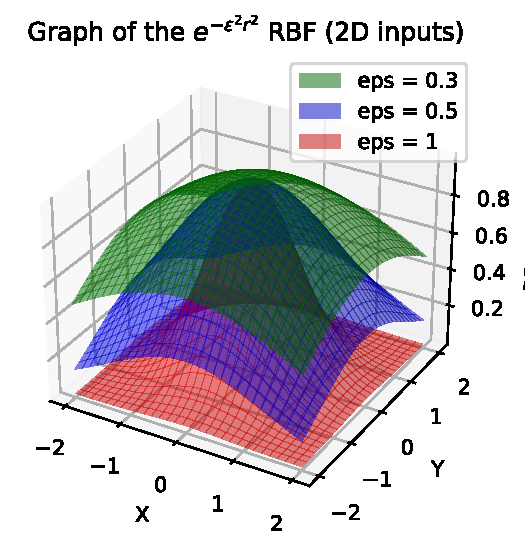
\includegraphics[width=.5\textwidth, clip=true, trim={0 0 .1cm 0}]{imagenes/rbf_discussion/negative-exp-rbf.pdf}}
  \caption{Representation of the radial basis function $e^{-\varepsilon^2 r^2}$. Note that a smaller value of $\varepsilon$ translates into a progressively flatter shape, whereas a larger value of $\varepsilon$ causes the function to feature a more stark cusp.}
  \label{fig:negative-exp-rbf}
\end{figure}

As the previous results show, one needs a firm grasp on Fourier transforms as well as
measure theory to reliably make use of these results and ultimately showing that
the Gaussian function is strictly positive definite. Because of this very reason, we turn
to the last set of (arguably more manageable) theoretical results.

% \subsection*{Characterizations in terms of completely monotone functions}

\begin{definition}
  A function $\varphi : [0, \infty) \rightarrow \mathbb{R}, \varphi \in C [0,
    \infty) \cap C^{\infty} (0, \infty)$ such that
  \[ (- 1)^{l} \varphi^{(l)} (r) \geq 0, \quad r > 0,
    l= 0, 1, 2, \ldots, \]
  is said to be {\tmstrong{completely monotone}} on $[0, \infty)$.
\end{definition}

\begin{theorem}
  \label{thm-completely-monotone-iff-positive-definite-radial}A function
  $\varphi : [0, \infty) \rightarrow \mathbb{R}$ is completely monotone on
  $[0, \infty)$ if and only if $\phi (\cdot) = \varphi (\| \cdot \|^2)$ is
  positive definite and radial on $\mathbb{R}^d$ for all $d$.
\end{theorem}

Note that Theorem \ref{thm-completely-monotone-iff-positive-definite-radial}
imposes a relation between functions $\phi$ and $\varphi$ different to that of
Definition \ref{radialfunctions}. Much like the work we did on Theorem
\ref{tm-bochner}, we will only prove the direction that yields the
positive-definiteness and ``radiality'' on $\mathbb{R}^d$ for all $d$. To this
end, we shall use the following Theorem:

\begin{theorem}
  {\tmstrong{(Hausdorff-Bernstein-Widder)}}\label{thm-hausdorff-bernstein-widder}
  A function $\varphi : [0, \infty) \rightarrow \mathbb{R}$ is completely
  monotone on $[0, \infty)$ if and only if it is the Laplace transform of a
  finite  Borel measure $\mu$ on $[0, \infty)$, that is, if
  \begin{equation}
    \varphi (r) = \int_0^{\infty} e^{- r t} d \mu (t) .
    \label{phi-thm-hausdorff}
  \end{equation}
\end{theorem}

\begin{proof}
  {\tmstrong{(Theorem
      \ref{thm-completely-monotone-iff-positive-definite-radial})}} Applying
  Theorem \ref{thm-hausdorff-bernstein-widder}, we can express $\varphi$ like
  in \eqref{phi-thm-hausdorff}, for a finite Borel measure $\mu$,
  or equivalently in terms of $\| \tmmathbf{x} \|^2$ by noting that $\phi
    (\tmmathbf{x}) = \varphi (\| \tmmathbf{x} \|^2)$. To conclude the positive
  definiteness of $\phi$, we simply check the definition and apply the
  linearity of the integral:
  \begin{equation}\label{eqn-linearity-of-integral}
    \sum_{j = 1}^N \sum_{k = 1}^N c_j c_k \phi (\tmmathbf{x}_j
    -\tmmathbf{x}_k) = \int_0^{\infty} \sum_{j = 1}^N \sum_{k = 1}^N c_j c_k
    e^{- t \| \tmmathbf{x}_j -\tmmathbf{x}_k \|^2} d \mu (t) .
  \end{equation}

  Noting that we integrate on $t \geq 0$, it follows that the quadratic form of
  the integrand involves Gaussian functions, which were shown in Example
  \ref{ex-gaussian-strictly-positive-definite} to be strictly positive
  definite. Consequently, the quadratic form is non-negative, which ultimately
  implies the positive definiteness of $\varphi$.
\end{proof}

\begin{theorem}
  If $\varphi$ is completely monotone but not constant on $[0,\infty)$,
  then the function ${\tmmathbf{x}} \mapsto \varphi(||\tmmathbf{x}||^2)$ is a radial,
  strictly positive definite function on any inner-product space.

  Thus, for any $n$ distinct points
  $\{\tmmathbf{x}_1,\tmmathbf{x}_2,...,\tmmathbf{x}_n\}$
  in such a space, the matrix
  $A_{i,j}=\varphi(||\tmmathbf{x}_i-\tmmathbf{x}_j||)$ is positive definite
  (and therefore nonsingular).
\end{theorem}

\begin{proof}
  Because $\varphi$ is completely monotone, Theorem
  \ref{thm-hausdorff-bernstein-widder} implies that there is a bounded Borel
  measure $\mu$ on $[0, \infty)$ for which \eqref{phi-thm-hausdorff} holds.
  Moreover, $\varphi$ is assumed not to be constant, which implies that $\mu (0,
    \infty) > 0$ and ultimately that $d \mu$ is not concentrated at $0$. Now,
  taking $A_{i, j} = \varphi (\| \tmmathbf{x}_i -\tmmathbf{x}_j \|^2)$ and any
  $c = (c_1, c_2, \ldots, c_n) \neq 0$, we again come upon
  \eqref{eqn-linearity-of-integral}. Recalling that the integrand is positive
  and that the measure is not concentrated at $0$, the result follows.
\end{proof}

In the following, we turn to formulating Problem \ref{interpolationproblemstatement}
with the definitions devised in Section \ref{sec-neural-networks}. Furthermore,
we shall explicitly propose examples to move the discussion forward and identify
concerns on the computational side of the Problem.

\section{Interpolation with RBFs and NN}

The radial basis function method for interpolating a function can then be
proposed and solved by means of a neural network. One of the first works at
this respect was the one carried out by Broomhead and Lowe in 1988
  {\cite{broomhead1988multivariable}}, where they expressed that the linear
dependence of the weights in the radial basis function expansion would allow
for a globally optimum least-squares interpolation of an arbitrary function.

To solve this problem, the multi-layer perceptron \eqref{perceptronRule}
(actually, a three-layer perceptron) was seen to fit the radial basis function
expansion \eqref{eqn-p-is-a-linear-combination-of-rbfs}. Indeed, suppose we want
to interpolate specific realizations of a map $f : \mathbb{R}^d \rightarrow
  \mathbb{R}$ with an RBF expansion of $N$ centers. In such case, multi-layer
perceptron theory allows one to define a function of the form
\[ \begin{array}{cccc}
    \mathcal{N}^3 : & \mathbb{R}^N & \rightarrow & \mathbb{R}                             \\
                    & \tmmathbf{x} & \mapsto     & \sigma_3 (\tmmathbf{W}^3 \mathcal{N}^2
    (\tmmathbf{x}) +\tmmathbf{b}^3)
  \end{array}, \]
where $\tmmathbf{W}^3 \in \mathbb{R}^{1 \times N}$ corresponds to our linear
coefficients $\lambda_1, \lambda_2, \ldots, \lambda_N$, $\tmmathbf{b}^3 \equiv
  \tmmathbf{0}$ and $\sigma_3$ denotes the entry-wise identity operator. By the
same token, we define
\[ \begin{array}{cccc}
    \mathcal{N}^2 : & \mathbb{R}^d & \rightarrow & \mathbb{R}^N                           \\
                    & \tmmathbf{x} & \mapsto     & \sigma_2 (\tmmathbf{W}^2 \mathcal{N}^1
    (\tmmathbf{x}) +\tmmathbf{b}^2)
  \end{array}, \]
where $\tmmathbf{W}^2 \in \mathbb{R}^{N \times d}$ is the identity operator,
$\tmmathbf{b}^2 \equiv \tmmathbf{0}$ and
\[ \sigma_2 (\tmmathbf{x}) = \left(\begin{array}{cccc}
    \varphi (\| \tmmathbf{x}-\tmmathbf{x}_1 \|) & \varphi (\|
    \tmmathbf{x}-\tmmathbf{x}_2 \|)             & \ldots      & \varphi (\|
    \tmmathbf{x}-\tmmathbf{x}_N \|)
  \end{array}\right)^{\top} \]
is the vector whose entries are the application of a certain RBF $\varphi$ to the input
$\tmmathbf{x}$ up to each of our $N$ centers. Consequently, the radial basis
function expansion may be expressed by means of Figure \ref{fig-rbf-drawing}.
\begin{figure}[ht]
  % \frame
  {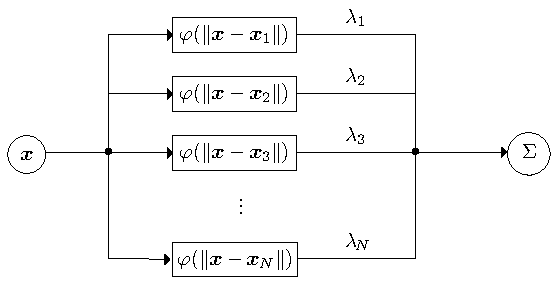
\includegraphics[width=.7\textwidth]{imagenes/rbf_discussion/rbf-nn-graph.pdf}}
  \caption{Depiction of a three-layer perceptron for RBF expansion. The
    initial layer is the input layer, the hidden layer denotes the application
    of the RBF function up to the $N$ centers (the previously-defined operator
    $\sigma_2$), and the final layer denotes their sum up to the coefficients
    $\lambda_1, \lambda_2, \ldots, \lambda_N$ (the previously-defined
    $\tmmathbf{W}^3 \in \mathbb{R}^{1 \times N}$).
    \label{fig-rbf-drawing}}
\end{figure}

So far the discussion has been devoted to tie the apparent distances between
the RBF expansion method with the multi-layer perceptron, to describe the
former in terms of the latter in order to apply well-known machine learning
methods to solve problems with RBFs. Unlike ``traditional'' multi-layer
perceptrons, whose leading idea is often the usage of nested affine
transformations and activation functions to try and solve complex problems
(with the usage of often complex architectures), radial basis function
expansions yield pithy mathematical forms to solve problems that would require
more than one affine transformation if we were to use this ``traditional''
multi-layer perceptron.

Such is the case of the \tmverbatim{xor} operator (``exclusive or''), a
binary operator that obeys the rule expressed in the left-hand side of Table
\ref{table-xor-distances}:

% \begin{table}[h]
%   \begin{tabular}{ll}
%     {\center{\begin{tabular}{|c|c|c|}
%       \hline
%       \tmverbatim{A} & \tmverbatim{B} & \tmverbatim{xor(A,B)}\\
%       \hline
%       0 & 0 & 0\\
%       \hline
%       0 & 1 & 1\\
%       \hline
%       1 & 0 & 1\\
%       \hline
%       1 & 1 & 0\\
%       \hline
%     \end{tabular}}} &
%     \frame
%     {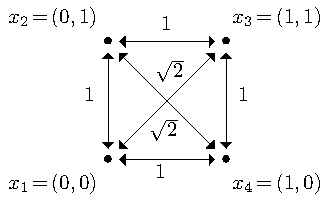
\includegraphics[width=.45\textwidth]{imagenes/rbf_discussion/drawing-xor.pdf}}
%   \end{tabular}
%   \caption{On the left-hand side, the explicit mapping of the \tmverbatim{xor}
%   function for any binary input. On the right-hand side, the localization of
%   the 2D inputs in a plane alongside their pairwise Euclidean distances.
%   \label{table-xor-distances}}
% \end{table}

\begin{table}[h]
  \begin{tabular}{ll}
    \frame
    {\begin{tabular}{|c|c|c|}
         \hline
         \tmverbatim{A} & \tmverbatim{B} & \tmverbatim{xor(A, B)} \\
         \hline
         0              & 0              & 0                      \\
         \hline
         0              & 1              & 1                      \\
         \hline
         1              & 0              & 1                      \\
         \hline
         1              & 1              & 0                      \\
         \hline
       \end{tabular}} &
    {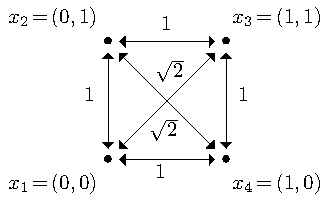
\includegraphics[width=.41\textwidth]{imagenes/rbf_discussion/drawing-xor.pdf}}
  \end{tabular}
  \caption{On the left-hand side, the explicit mapping of the \tmverbatim{xor}
    function for any binary input. On the right-hand side, the localization of
    the 2D inputs in a plane alongside their pairwise Euclidean distances.
  }
  \label{table-xor-distances}
\end{table}

Notice that the two pairs of points for which we wish to produce the same
output always maximize their distance (see right-hand side of Table
\ref{table-xor-distances}). This immediately shows the unfeasibility of using
a single hyperplane as a classifier (i.e., as a function returning either 0 or
1 for our inputs). In other words: we cannot solve this problem by means of a
single affine transformation.

However, we can solve this problem in terms of an RBF expansion, that is, in
terms of a neural network with a single hidden layer. To this end, note that
we have defined the \tmverbatim{xor} operator by extension: there are exactly
four bi-dimensional possible inputs. It is in those inputs where our centers will be located.
Considering so far an arbitrary radial basis function $\varphi (\| \cdot \|)$
and operating under the Euclidean norm, we wish to find a function $\sum_{i =
    1}^4 \lambda_i \varphi (\| \tmmathbf{x}-\tmmathbf{x}_j \|_2)$, where
$\tmmathbf{x}_1, \tmmathbf{x}_2, \tmmathbf{x}_3, \tmmathbf{x}_4$ are distanced as in the
right-hand side of Table \ref{table-xor-distances}. Consequently,
\eqref{eqn-linear-system-equations-rbf} is now expressed as
\begin{equation}
  \left(\begin{array}{cccc}
      \varphi (0)                       & \varphi (1)                     & \varphi \left( \sqrt{2} \right) & \varphi
      (1)                                                                                                                             \\
      \varphi (1)                       & \varphi (0)                     & \varphi (1)                     & \varphi \left( \sqrt{2}
      \right)                                                                                                                         \\
      \varphi \left( \sqrt[]{2} \right) & \varphi (1)                     & \varphi (0)                     & \varphi
      (1)                                                                                                                             \\
      \varphi (1)                       & \varphi \left( \sqrt{2} \right) & \varphi (1)                     & \varphi (0)
    \end{array}\right) \left(\begin{array}{c}
      \lambda_1 \\
      \lambda_2 \\
      \lambda_3 \\
      \lambda_4
    \end{array}\right) = \left(\begin{array}{c}
      0 \\
      1 \\
      0 \\
      1
    \end{array}\right) .\label{interpolationconditionxor}
\end{equation}

Calling $A$ the real symmetric matrix on the left-hand side of the equation,
and under suitable radial basis functions such that $A$ is full rank, we have
$A = V \mu V^{\top}$ with $V$ an orthogonal matrix (which is such that $V^{\top} =
  V^{- 1}$) and $\mu$ a diagonal matrix with nonzero entries. Therefore, we can
compute the inverse of $A$ by means of the matrix product
\begin{equation}
  A^{- 1} = V \mu^{- 1} V^{\top} . \label{eqn-a-inverse-eigenvectors}
\end{equation}
Actually, we can find an analytic expression\footnote{Refer to Appendix A of
    {\cite{broomhead1988multivariable}} (Table 2 and equations A.4, A.5) for precise computation details.} for $V$
and $\mu$, which ultimately allows us to solve for $A$. It is
\[ V = \frac{1}{2} \left(\begin{array}{rrrr}
      1 & 1   & \sqrt{2}   & 0          \\
      1 & - 1 & 0          & - \sqrt{2} \\
      1 & 1   & - \sqrt{2} & 0          \\
      1 & - 1 & 0          & - \sqrt{2}
    \end{array}\right), \text{ alongside } \]
\begin{equation}
  \mu = \left(\begin{array}{cccc}
      \mu_1 & 0     & 0     & 0     \\
      0     & \mu_2 & 0     & 0     \\
      0     & 0     & \mu_3 & 0     \\
      0     & 0     & 0     & \mu_3
    \end{array}\right), \text{ for } \left\{\begin{array}{l}
    \mu_1 = \varphi (0) + 2 \varphi (1) + \varphi \left( \sqrt{2} \right) \\
    \mu_2 = \varphi (0) - 2 \varphi (1) + \varphi \left( \sqrt{2} \right) \\
    \mu_3 = \varphi (0) - \varphi \left( \sqrt{2} \right)
  \end{array}\right. . \label{eqn-mu-analytic-eigenvector}
\end{equation}
Because $V$ is an orthogonal matrix, the existence of $A^{- 1}$ is tied to the
existence of $\mu^{- 1}$, as per \eqref{eqn-a-inverse-eigenvectors}. This is
equivalent to say that we need $\mu_1, \mu_2, \mu_3$ to be nonzero, which
entirely depends on the choice of $\varphi$: reasoning on
\eqref{eqn-mu-analytic-eigenvector}, we note that $\mu_3 = 0 \Leftrightarrow
  \varphi (0) = \varphi \left( \sqrt{2} \right)$. Likewise, $\mu_1 = 0
  \Leftrightarrow \varphi (1) = - \frac{\varphi (0) + \varphi \left( \sqrt{2}
    \right)}{2}$ and $\mu_2 = 0 \Leftrightarrow \varphi (1) = \frac{\varphi (0) +
    \varphi \left( \sqrt{2} \right)}{2}$. Provided we have carefully chosen the
RBFs to avoid null eigenvalues, we may explicitly compute the parameters
vector $\underline{\lambda}$ as in \eqref{matrixexpression-interpolationprob}
for problem \eqref{interpolationconditionxor}. To this end, let $f = (0, 1, 0,
  1)^{\top}$ denote the right-hand side column vector (to be expressed in terms of the orthogonal vectors conforming $V$), whereupon
\[ \underline{\lambda} = A^{- 1} f = V \mu^{- 1} V^{\top} f = V \mu^{- 1}
  V^{\top} \frac{1}{2} \left[ \left(\begin{array}{c}
      1 \\
      1 \\
      1 \\
      1
    \end{array}\right) - \left(\begin{array}{r}
      1   \\
      - 1 \\
      1   \\
      - 1
    \end{array}\right) \right] = V \mu^{- 1} \left[ \left(\begin{array}{c}
      1 \\
      0 \\
      0 \\
      0
    \end{array}\right) - \left(\begin{array}{c}
      0 \\
      1 \\
      0 \\
      0
    \end{array}\right) \right] = \]
\[ = V \left(\begin{array}{r}
      \mu_1^{- 1}   \\
      - \mu_2^{- 1} \\
      0             \\
      0
    \end{array}\right) = \frac{1}{2} \left(\begin{array}{c}
      \mu_1^{- 1} - \mu_2^{- 1} \\
      \mu_1^{- 1} + \mu_2^{- 1} \\
      \mu_1^{- 1} - \mu_2^{- 1} \\
      \mu_1^{- 1} + \mu_2^{- 1}
    \end{array}\right) \Rightarrow \underline{\lambda} = \left(\begin{array}{c}
      \lambda_1 \\
      \lambda_2 \\
      \lambda_3 \\
      \lambda_4
    \end{array}\right) = \left(\begin{array}{c}
      \lambda_1 \\
      \lambda_2 \\
      \lambda_1 \\
      \lambda_2
    \end{array}\right) . \]
Substituting now \eqref{eqn-mu-analytic-eigenvector} in this last equation and expanding, we
conclude that \begin{equation}
  \lambda_1 = - \frac{2 \varphi (1)}{\left( \varphi (0) + \varphi
    \left( \sqrt{2} \right) \right)^2 - 4 \varphi (1)^2}, \text{ and } \lambda_2 =
  \frac{\varphi (0) + \varphi \left( \sqrt{2} \right)}{\left( \varphi (0) +
    \varphi \left( \sqrt{2} \right) \right)^2 - 4 \varphi (1)^2}.
  \label{eqn-lda1-lda2}
\end{equation}

\begin{figure}[ht]
  \centering
  \begin{tabular}{ll}
    % \frame
    {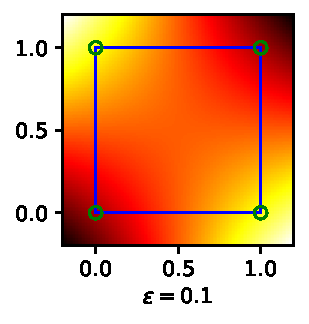
\includegraphics[width=.33\textwidth]{imagenes/xor/xor0.1.pdf}} & 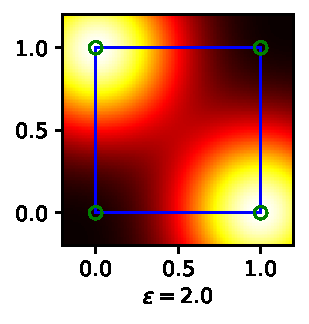
\includegraphics[width=.33\textwidth]{imagenes/xor/xor2.0.pdf} \\
    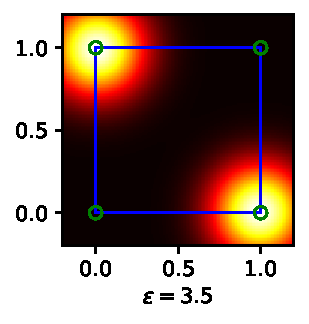
\includegraphics[width=.33\textwidth]{imagenes/xor/xor3.5.pdf}   & 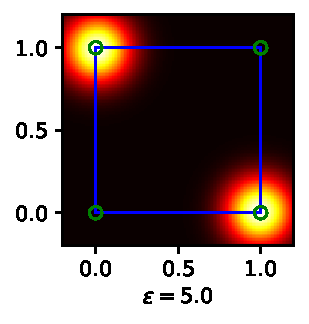
\includegraphics[width=.33\textwidth]{imagenes/xor/xor5.0.pdf}
  \end{tabular}
  \begin{tabular}{r}
    % \frame
    {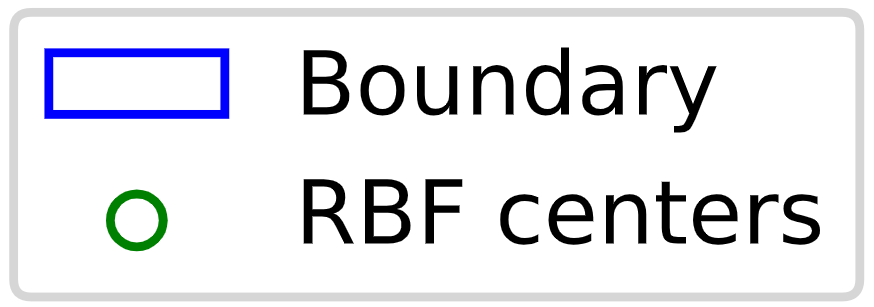
\includegraphics[width=.24\textwidth, trim={0 -2cm 0 0}, clip=true]{imagenes/xor/Legend.png}}
    \\
    {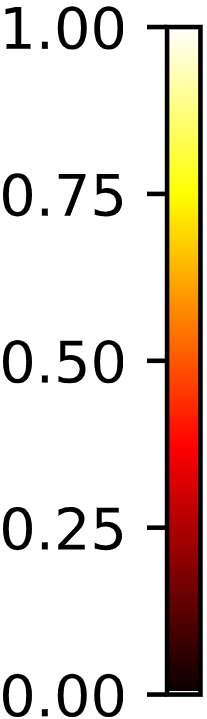
\includegraphics[height=.4\textwidth]{imagenes/xor/Colorbar.png}}
  \end{tabular}
  \caption{Contour of the \texttt{xor} binary operator with a Gaussian RBF expansion for different values of the shape parameter $\varepsilon$. In coherence with Figure \ref{fig:negative-exp-rbf}, larger values of $\varepsilon$ translate into starker cusps (see figures for $\varepsilon=3.5,5.0$).}
  \label{fig:xor}
\end{figure}

We refer to Figure \ref{fig:xor} for a comparison on the interpolation of the
four values provided for the \tmverbatim{xor} operator with a Gaussian RBF
under different values of the shape parameter $\varepsilon$. If we were
instead dealing in a fuzzy logic\footnote{See {\cite{zadeh1988fuzzy}} or
    {\cite{russell2005ai}} for starting pointers.} setting, whereby the truth
value of a statement would now take values in $[0, 1]$, the shape parameter
would be instrumental in determining an appropriate set of such intermediate
truth values. One must bear in mind that this example, where we have been able
to determine an explicit form of $\underline{\lambda}$ without explicitly
inverting matrix $A$, is not going to happen in general.

\begin{definition}
  Let $A \in \mathbb{R}^{n \times n}$. The number
  \[ \kappa_{\| \cdot \|} (A) = \| A^{- 1} \| \cdot \| A \| \]
  is said to be the {\tmstrong{condition number}} for inverting $A$ under the
  norm $\| \cdot \|$.
\end{definition}

Provided we wish to solve a system of the form $A \underline{\lambda} = f$,
with $A, \underline{\lambda} \text{ and } f$ as in
\eqref{eqn-linear-system-equations-rbf}, our previous discussion shows that there
are two key components that determine the condition number of the inversion of
$A$: the particular {\tmstrong{choice of RBFs}} and the {\tmstrong{location of
      the centers}}. We address the former component for now.

To this end, we refer to the left-hand side of Figure
\ref{fig:xor-coefficients-conditioning} and note that the condition number of
the inverse increases linearly as $\varepsilon$ ranges (roughly) from $1$ to
$10^{- 1}$. Further reducing the value of the shape parameter cues in an
ill-conditioned problem, for which the condition number of the matrix
notoriously oscillates. This ultimately causes the coefficients of the RBF
expansion to increase in orders of magnitude {\cite{fornberg2015primer}}, as
the right-hand side of Figure \ref{fig:xor-coefficients-conditioning} shows.
Consequently, if we are to optimize the parameters of a neural network
implemented as in \ref{fig-rbf-drawing} (which is a direct implementation of
the RBF expansion), the search for suitable coefficients to solve the
interpolation problem of the \tmverbatim{xor} operator would see us choosing
some shape parameter $\varepsilon > 1$.

This observation leads us now into the search for other RBFs, with (maybe)
more suitable condition numbers for the inversion of the matrix of the
scattered data interpolation problem.

\begin{figure}[ht]
  \centering
  % \frame
  {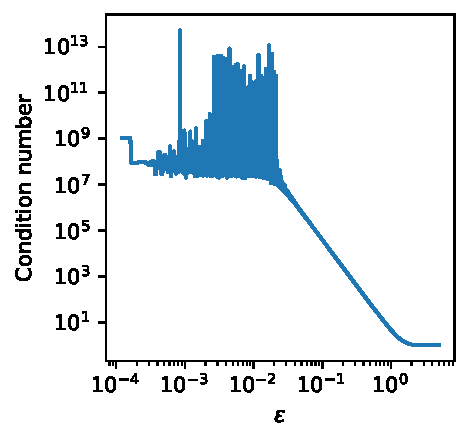
\includegraphics[width=.45\textwidth]{imagenes/xor/xor_conditioning_graph.pdf}}
  {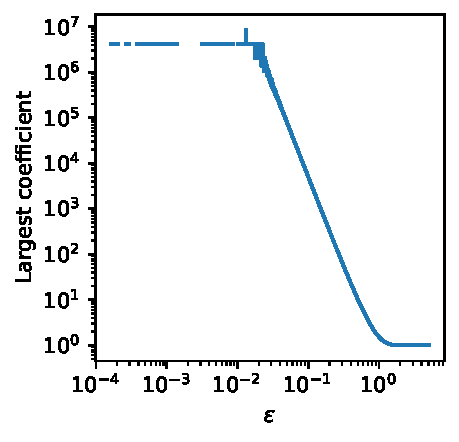
\includegraphics[width=.45\textwidth]{imagenes/xor/xor_largest_coef_graph.pdf}}
  \caption{Left-hand side: the condition number of the inversion of matrix $A$ of the \texttt{xor} binary operator interpolation problem. Right-hand side: order of magnitude of the largest (in absolute value) coefficient of the RBF expansion. Note that the ``empty'' values in the right-hand side figure are due to the numerical computation of the coefficients $\lambda_1, \lambda_2$ in \eqref{eqn-lda1-lda2} returning a value too large for the system's floating point system, which then defaults to infinity.}
  \label{fig:xor-coefficients-conditioning}
\end{figure}

To this end, following Micchelli's discussion \cite{micchelli1984interpolation} we generalize the radial basis function expansion \eqref{eqn-p-is-a-linear-combination-of-rbfs} into the form
\begin{equation}
  \mathcal{P} (\tmmathbf{x}) = \sum_{i = 1}^N \lambda_i \phi_j (\tmmathbf{x})
  + \sum_{i = 1}^m \mu_i p_i (\tmmathbf{x}), \quad m \leq n,
  \label{eqn-rbf-poly}
\end{equation}
where each $\phi_j : \mathbb{R}^d \rightarrow \mathbb{R}$ is such that
$\phi_j (\tmmathbf{x}) = \varphi (\| \tmmathbf{x}-\tmmathbf{x}_j \|)$ for a
fixed $\tmmathbf{x}_j \in \mathbb{R}^d$ and $\varphi : [0, \infty) \rightarrow
  \mathbb{R}$ is a continuous function. Furthermore, we prescribe that
$\tmop{span} \{ p_1, p_2, \ldots, p_m \}$ should be equal to $\mathbb{P}_{k -
    1} (\mathbb{R}^d)$, the space of polynomials of total degree $\leq k - 1$.



\begin{definition}\label{def-rbf-poly}
  Let $\varphi : [0, \infty) \rightarrow \mathbb{R}$ be a continuous function,
  $\{ \tmmathbf{x}_j \}_{j = 1}^N \subset \mathbb{R}^d$ a set of distinct
  points and $(\lambda_1, \lambda_2, \ldots, \lambda_N) \in \mathbb{R}^N$ such
  that
  \begin{equation}
    \sum_{i = 1}^N \lambda_i p (\tmmathbf{x}_i) = 0
    \label{constraint-rbf-polynomial}
  \end{equation}
  for all $p \in \mathbb{P}_{k - 1} (\mathbb{R}^d)$. If the quadratic form
  \[ \sum_{i = 1}^N \sum_{j = 1}^N \lambda_i \lambda_j \varphi (\|
    \tmmathbf{x}_i -\tmmathbf{x}_j \|) \]
  is non-negative (resp., positive), then $\varphi$ is said to be
    {\tmstrong{conditionally positive}} (resp. {\tmstrong{conditionally strictly
        positive}}) {\tmstrong{definite of order $k$}} on $\mathbb{R}^d$.
\end{definition}

% We now extend Theorem
% \ref{thm-completely-monotone-iff-positive-definite-radial} to functions of the
% form \eqref{eqn-rbf-poly}.

\begin{theorem}
  If $\varphi \in C [0, \infty)$ and $(- 1)^k \varphi^k(r)$ is
  completely monotone on $(0, \infty)$, then $\varphi$ is conditionally
  positive of order $k$.
\end{theorem}

For the sake of clarity, \eqref{constraint-rbf-polynomial} can be formulated
as
\[ \sum_{i = 1}^N \lambda_i = \sum_{i = 1}^N \lambda_i x_i = \sum_{i = 1}^N \lambda_i
  x^2_i = \cdots = \sum_{i = 1}^N \lambda_i x^m_i = 0, \]
which allows one to consider the system
\[ \left[\begin{array}{ccc|ccccc}
                                  &        &                             & {\color[HTML]{008000}1} & {\color[HTML]{008000}x_1} &
      {\color[HTML]{008000}x_1^2} & \ldots & {\color[HTML]{008000}x_1^m}                                                                            \\
                                  & A      &                             & \vdots                  & \vdots                    & \vdots &  & \vdots \\
                                  &        &                             & {\color[HTML]{008000}1} & {\color[HTML]{008000}x_N} &
      {\color[HTML]{008000}x_N^2} & \ldots & {\color[HTML]{008000}x_N^m}                                                                            \\ \hline
      1                           & \ldots & 1                           &                         &                           &        &  &        \\
      x_1                         & \ldots & x_N                         &                         &                           &        &  &        \\
      x_1^2                       & \ldots & x_N^2                       &                         &                           & 0      &  &        \\
      \vdots                      &        & \vdots                      &                         &                           &        &  &        \\
      x_1^m                       & \ldots & x_N^m                       &                         &                           &        &  &
    \end{array}\right] \left[\begin{array}{c}
      \lambda_1 \\
      \vdots    \\
      \lambda_N \\
      \hline
      \mu_1     \\
      \mu_2     \\
      \mu_3     \\
      \vdots    \\
      \mu_m
    \end{array}\right] = \left[\begin{array}{c}
      f_1    \\
      \vdots \\
      f_N    \\
      \hline
      0      \\
      0      \\
      0      \\
      \vdots \\
      0
    \end{array}\right] \]
expressed in the more compact notation
\begin{equation}
  \left[\begin{array}{cc}
      A        & P            \\
      P^{\top} & \tmmathbf{0}
    \end{array}\right] \left[\begin{array}{c}
      \underline{\lambda} \\
      \underline{\mu}
    \end{array}\right] = \left[\begin{array}{c}
      \underline{f} \\
      \tmmathbf{0}
    \end{array}\right]. \label{eqn-augmented-rbf-poly-system}
\end{equation}

The submatrix with entries in green is of dimensions $n \times (m + 1)$. Therefore, the
resulting matrix is square and of size $(m + n + 1) \times (m + n + 1)$.

We will return to these functions in the coming discussions. For now, we turn to another set of results, which will allow us to present the \textbf{multiquadric} radial basis function. To do so, we follow the discussion presented in \cite{sarra2009multiquadric}:

\begin{theorem}
  Assume $\varphi'(r)$ is completely monotone and not constant on
  $(0, \infty)$, $\varphi \in C [0, \infty)$ and $\varphi (r) > 0$ for $r >
    0$. Denote by $A$ the matrix in \eqref{eqn-linear-system-equations-rbf}. Then,
  for any distinct $\{ \tmmathbf{x}_j \}_{j = 1}^N \subset \mathbb{R}^d$
  \[ (- 1)^{N - 1} \det A > 0, \]
  which implies the invertibility of $A$.
  \label{thm-A-invertible}
\end{theorem}

\begin{example}
  Under these few new results, and letting $m = 0$ in \eqref{eqn-rbf-poly},
  one can already consider the multiquadric (MQ) radial basis function,
  $\varphi (r) = \sqrt{1 + \varepsilon^2 r} > 0$. Note that
  \[ \begin{array}{ccl}
      \varphi' (r)      & = & \frac{\varepsilon^2}{2} (\varepsilon^2 r + 1)^{- 1 /
      2}                                                                           \\
      \varphi'' (r)     & = & - \frac{\varepsilon^4}{4} (\varepsilon^2 r + 1)^{-
      3 / 2}                                                                       \\
      \varphi''' (r)    & = & \frac{3 \varepsilon^6}{8} (\varepsilon^2 r + 1)^{-
      5 / 2}                                                                       \\
      \varphi^{(4)} (r) & = & - \frac{15 \varepsilon^8}{16} (\varepsilon^2 r
      + 1)^{- 7 / 2}
    \end{array} . \]
  We observe that $(- 1)^l \varphi^{(l)} (r) \leq 0$ for all $r \geq 0$ and $l
    = 0, 1, 2, \ldots$, due to the changes in sign introduced by the derivative
  with respect to $r$ of $(\varepsilon^2 r + 1)^{- \beta}, \beta > 0$. It
  follows that $\varphi' (r)$ is completely monotone. It is also immediate to
  see that $\varphi' (r) > 0$ is not constant. Finally, the largest possible
  domain of $\varphi$ is $r \geq - 1 / \varepsilon^2$, for which it also is
  continuous. Since we assume $r \geq 0$, Theorem \ref{thm-A-invertible}
  guarantees the invertibility of the corresponding the interpolation matrix for
  any scattered data interpolation problem.
\end{example}

It is common to consider also this multiquadric RBF under the formulation
$\varphi (r) = \sqrt{1 + \varepsilon^2 r^2}$. We depict this alternative in
Figure \ref{fig:mq-rbf} under different values of the shape parameter
$\varepsilon$.

\begin{figure}[ht]
  \centering
  % \frame
  {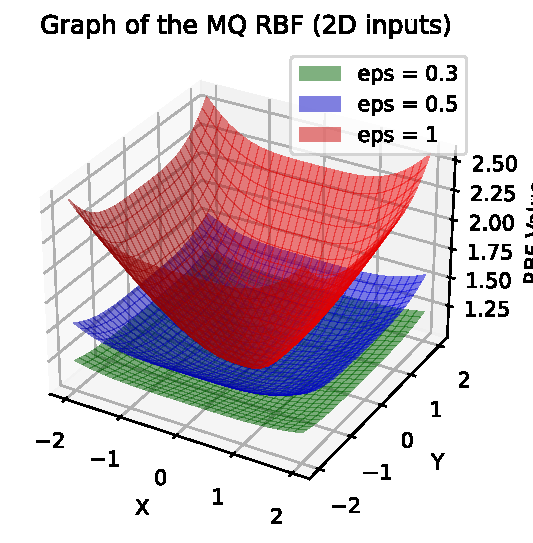
\includegraphics[width=.5\textwidth, clip=true, trim={0 0 .17cm 0}]{imagenes/rbf_discussion/mq-rbf.pdf}}
  \caption{Representation of the multiquadric radial basis function $\sqrt{1+\varepsilon^2 r^2}$. Much like in the case \ref{fig:negative-exp-rbf}, that a smaller value of $\varepsilon$ translates into a progressively flatter shape, whereas a larger value of $\varepsilon$ causes the function to feature a more stark cusp.}
  \label{fig:mq-rbf}
\end{figure}

\subsection*{Some ``pathological'' examples}

As pointed out in Theorem \ref{thm-haar-spaces-polynomials}, pre-fixed
generalized polynomials are not apt for interpolation problems of
dimension larger than one. Polynomials\footnote{We are not referring to generalized polynomials in this stretch of the discussion.}, which
have not been discussed up until now, can still be used for one-dimensional
problems. This is the motivation behind the next case study, where we consider
$x \mapsto \frac{1}{1 + 25 x^2}$, referred to as the {\tmstrong{Runge
      function}}. Figure \ref{fig:runge-polynomial-interpolation} depicts the
interpolation of this function on a progressively more populated equispaced
grid, which increases the degree of the interpolating polynomial under consideration\footnote{Experiment generated in the context of the \href{https://github.com/heqro/tfm-experiments/blob/main/introductory_notebooks/polynomial_interpolation/runge.ipynb}{polynomial interpolation notebook} featured in the repository.}.

Prior to seeing this depiction, one could mistakenly believe that supplying a larger number of interpolation points would decrease the error in between the interpolation nodes. For this particular function, it can be easily seen such is not the case. For instance, the interpolating polynomial of degree $10$ can be seen to reach large values for inputs close to the boundary of the problem\footnote{On a second (deeper) thought, this phenomenon is not that surprising: if the only information we provide is the value of the function at very specific nodes, we do not necessarily know the value of the interpolator at ``intermediate points''.}. However, the following Theorem states that a suitable polynomial can still be found:

\begin{figure}[ht]
  \centering
  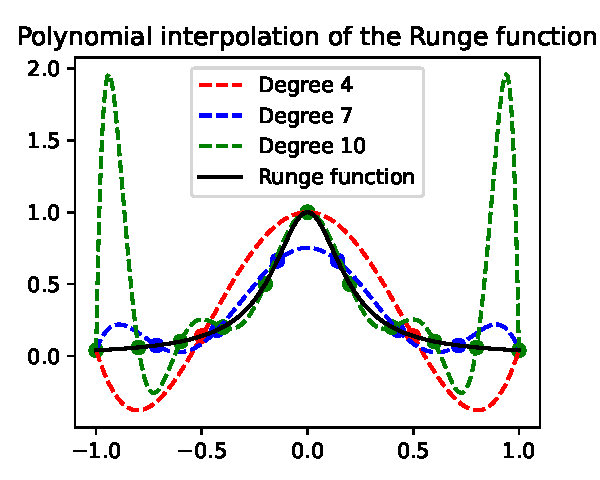
\includegraphics[width=.55\textwidth]{imagenes/polynomial_interpolation/Runge_Polynomial_interpolation.pdf}
  \caption{Polynomial interpolation of the Runge function with $n=5,8,11$ equispaced points. As one can see, larger degrees of the interpolating polynomial do not necessarily imply that the approximation will be close to the actual function between each pair of interpolation nodes.}
  \label{fig:runge-polynomial-interpolation}
\end{figure}

\begin{theorem}
  \label{thm-polynomial-convergence}Let $f$ be a continuous function defined
  on $[a, b]$. For all $\varepsilon > 0$ there corresponds a polynomial $P$
  such that $\| f - P \|_{\infty} < \varepsilon$.
\end{theorem}

A proof of this Theorem is featured in \cite{cheney1966introduction}, where an explicit form of $P$ is given by means of the sequence of
\textbf{Bernstein polynomials}, defined for each $n \in \mathbb{N}$ as
\begin{equation}
  (B_n f) (x) = \sum_{k = 0}^n f \left( \frac{k}{n} \right) \binom{n}{k} x^k
  (1 - x)^{n - k} \label{eqn-bernstein-polynomial},
\end{equation}
for $x \in [0, 1]$. After proposing this polynomial, it is shown that $B_n$ is
a monotone operator. Recall that an operator $L$ is said to be monotone if $f
  \geq g \Rightarrow L f \geq L g$. Assuming that, for any $n\in \mathbb{N}$ the operator $B_n$ is monotone, the following Theorem can be
used:

\begin{theorem}
  \label{thm-monotone-operators}Let $L_n \subset C [a, b]$ be a sequence of
  monotone linear operators. The following conditions are equivalent:
  \begin{enumerate}
    \item $L_n f \rightarrow f$ (uniformly) for all $f \in C [a, b]$.
    \item $L_n f \rightarrow f$ for $f (x) = 1, x, x^2$.
    \item $L_n 1 \rightarrow 1$ and $(L_n \phi_t) (t) \rightarrow 0$ uniformly
          in $t$, where $\phi_t (x) = (t - x)^2$.
  \end{enumerate}

\end{theorem}

\begin{proof}
  ({\tmstrong{Theorem}} \ref{thm-polynomial-convergence}) It suffices to show
  that the second property of Theorem \ref{thm-monotone-operators} holds.
  To this end, note that
  \[ (B_n 1) (x) = \sum_{k = 0}^n \binom{n}{k} x^k (1 - x)^{n - k} = [x + (1 -
        x)]^n = 1^n = 1. \]
  For $f (x) = x$, note that
  \[ (B_n f) (x) = \sum_{k = 0}^n \frac{k}{n} \binom{n}{k} x^k (1 - x)^{n - k}
    = x \sum_{k = 1}^n \binom{n - 1}{k - 1} x^{k - 1} (1 - x)^{n - k} = x
    \sum_{k = 0}^{n - 1} \binom{n - 1}{k} x^k (1 - x)^{n - 1 - k} = \]
  \[ = x (x + (1 - x))^{n - 1} = x. \]
  Finally, for $f (x) = x^2$ we have that
  \[ (B_n f) (x) = \sum_{k = 0}^n \left( \frac{k}{n} \right)^2 \binom{n}{k}
    x^k (1 - x)^{n - k} = \sum_{k = 1}^n \frac{k}{n} \binom{n - 1}{k - 1} x^k
    (1 - x)^{n - k} = \]
  \[ = \frac{n - 1}{n} \sum_{k = 1}^n \frac{k - 1}{n - 1} \binom{n - 1}{k - 1}
    x^k (1 - x)^{n - k} + \frac{1}{n} \sum_{k = 1}^n \binom{n - 1}{k - 1} x^k
    (1 - x)^{n - k} = \frac{n - 1}{n} x^2 + \frac{1}{n} x \xrightarrow[n]{}
    x^2 . \]
  Consequently, $B_n f \rightarrow f$ uniformly for all $f \in C [0, 1]$.
\end{proof}

The left-hand side of Figure \ref{fig:bernstein-runge} shows the absolute error when using Bernstein polynomials to approximate the Runge function\footnote{Experiment generated in the context of the \href{https://github.com/heqro/tfm-experiments/blob/main/introductory_notebooks/bernstein_polynomials/bernstein.ipynb}{Bernstein polynomial interpolation notebook} featured in the repository. We operate with the Runge function, albeit scaled to fit in the $[0,1]$ interval.}. Notice that we indeed have uniform convergence: for increasing values of $n$ as in \eqref{eqn-bernstein-polynomial}, the $L^\infty-$norm with respect to the Runge function decreases.

However, the right-hand side of this same picture allows us to confirm the shortcomings of Bernstein polynomials, which are due to rounding errors. For instance, cancellation occurs for large enough values of $n$ and $k$, which may in turn cause the evaluation of $(1-x)^{n-k}$ to default to $(1-x)$, altering the final result.

\begin{figure}[ht]
  \centering
  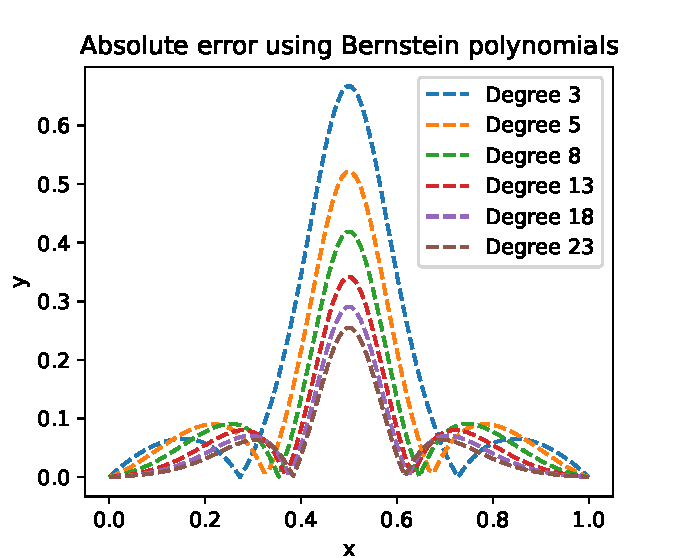
\includegraphics[width=.5\textwidth]{imagenes/bernstein/Bernstein_Polynomials_Runge.pdf}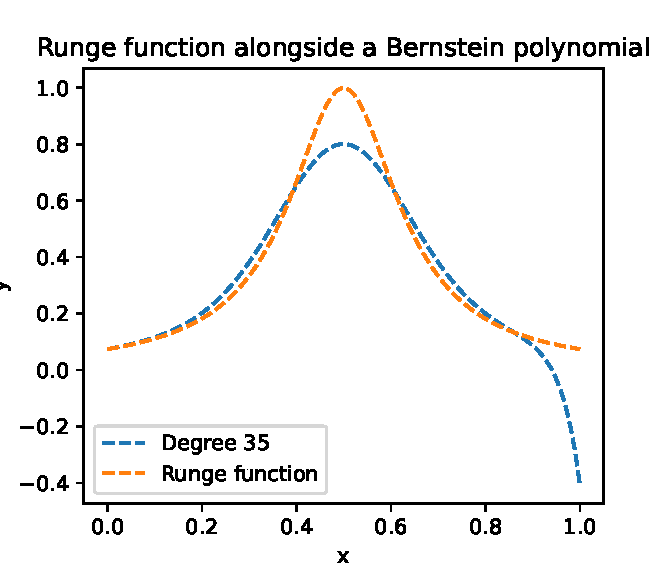
\includegraphics[width=.5\textwidth]{imagenes/bernstein/Bernstein_Polynomials_Runge_D35.pdf}
  \caption{Left-hand side: absolute error when using Bernstein polynomials of progressively higher degrees to approximate the Runge function. Right-hand side: a representation of the Runge function alongside a polynomial of higher degree.}
  \label{fig:bernstein-runge}
\end{figure}

Lastly, dismissing for a moment the computational issues and regarding only the mathematical framework, this polynomial \textit{happens} to be an interpolating polynomial because it can approximate the function to an arbitrary precision, but it requires us to provide an amount of information that is not proper of a scattered data interpolation problem, which ultimately rules out its utility for an interpolation task.

An effective alternative that does not involve Bernstein polynomials comes
from the consideration of a different set of interpolation points, the
so-called {\tmstrong{Chebyshev nodes}}. A set of Chebyshev nodes featuring $n$
points is defined as the family
\begin{equation}
  \left\{ \cos \left( \frac{2 k + 1}{2 n} \cdot \pi \right) \right\}_{k =
  0}^{n - 1} \label{eqn-chebyshev-nodes} \subset (- 1, 1),
\end{equation}
depicted in Figure \ref{fig:chebyshev-nodes}.

\begin{figure}[ht]
  \centering
  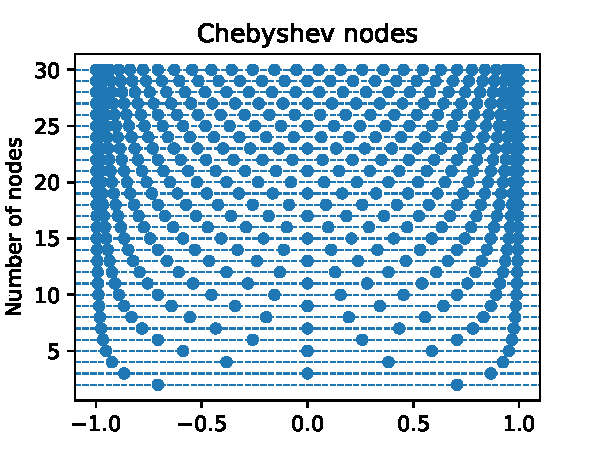
\includegraphics[width=.5\textwidth]{imagenes/polynomial_interpolation/Chebyshev_Nodes.pdf}
  \caption{Distribution of Chebyshev nodes alongside the horizontal axis for an increasing number of nodes.}
  \label{fig:chebyshev-nodes}
\end{figure}



Applying these nodes to the
interpolation of the Runge function\footnote{Experiment generated in the context of the \href{https://github.com/heqro/tfm-experiments/blob/main/introductory_notebooks/polynomial_interpolation/runge_chebyshev.ipynb}{Chebyshev nodes polynomial interpolation notebook} featured in the repository.} (as depicted in Figure
\ref{fig:runge-polynomial-cheb}) shows the effectiveness of the strategy,
whereby we have managed to severely reduce the oscillations between each pair
of interpolation nodes up to the point of guaranteeing a relative error
smaller than $10^{- 1}$ in the case we consider $n = 20$ points.

\begin{figure}[ht]
  \centering
  % \frame
  {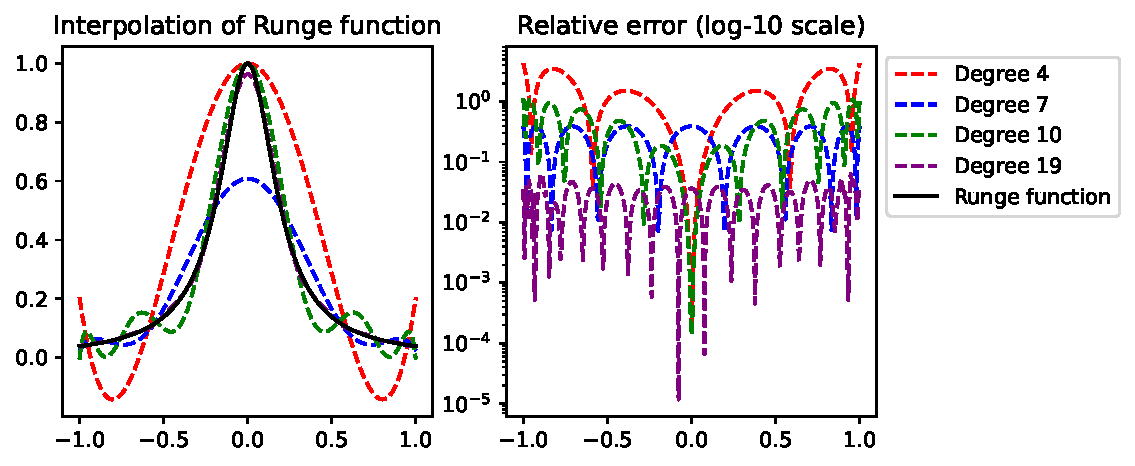
\includegraphics[width=\textwidth]{imagenes/polynomial_interpolation/Runge_Polynomial_Cheb.pdf}}
  \caption{Left-hand side: polynomial interpolation of the Runge function for $n=5, 8, 11, 20$ points distributed as in \eqref{eqn-chebyshev-nodes}. Right-hand side: the corresponding relative error in logarithmic scale.}
  \label{fig:runge-polynomial-cheb}
\end{figure}

As a side note,
it is not strictly necessary to resample the function over the new points of interest. That is, one may re-map the $x-$values of the function to the Chebyshev points while keeping the $y-$values intact and further reducing the oscillations. See for instance \cite{DEMARCHI2021125628} and, most interestingly, their proposed \href{https://github.com/pog87/FakeNodes/blob/master/Runge.ipynb}{associated code sample} for the Runge function.

Gaussian RBFs are able to further reduce this oscillation problem without the need of considering a separate points distribution. Figure \ref{fig:rbf-runge-phenomenon-eps-5-discussion} generated in the context of the linked \href{https://github.com/heqro/tfm-experiments/blob/main/introductory_notebooks/rbf_interpolation/runge_rbf.ipynb}{Gaussian RBF interpolation notebook} depicts that precision up to the first decimal place can be guaranteed, for instance, by considering 9 equispaced centers alongside a suitable shape parameter $\varepsilon=5$.

\begin{figure}[ht]
  \centering
  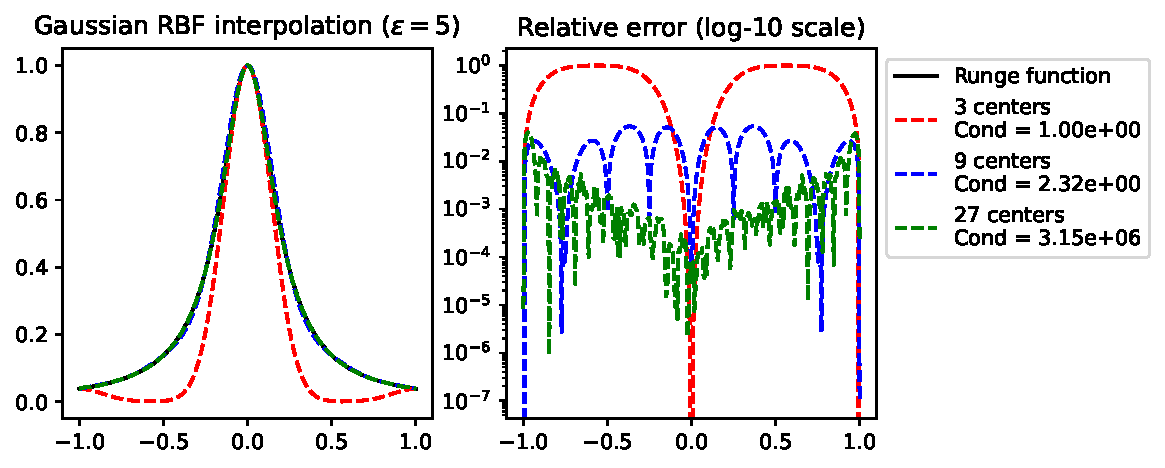
\includegraphics[width=\textwidth]{imagenes/rbf_interpolation/rbf_runge_5.pdf}
  \caption{Left-hand side: Gaussian RBF interpolation of the Runge function for $n=3,9,27$ equispaced points and $\varepsilon=5$. Right-hand side: relative error in logarithmic scale. Furthermore, the legend depicts the condition number of the matrix inversion problem.}
  \label{fig:rbf-runge-phenomenon-eps-5-discussion}
\end{figure}

As previously mentioned, the shape parameter plays a decisive role in the condition number of the matrix. For instance, refer to Figure \ref{fig:rbf-runge-phenomenon-eps-7} in the appendix for the corresponding results for $\varepsilon=7$. Indeed, the increment of the shape parameter reduces the condition number of the interpolation matrix for 27 centers in three orders of magnitude. Furthermore, the $L^\infty-$norm of the interpolation for 9 centers has visibly increased. Conversely, Figures \ref{fig:rbf-runge-phenomenon-eps-3} and \ref{fig:rbf-runge-phenomenon-eps-1} depict the situation for $\varepsilon=3,1$ respectively, whereby smaller values for $\varepsilon$ lead us to severe numerical errors.

To avoid explicitly choosing a shape parameter, \textbf{polyharmonic splines} (PHS) are defined by equipping a polynomial of degree larger than the unit to a suitable radial function, usually chosen $r^m,m$ odd, as in \eqref{eqn-rbf-poly}. We refer to Figures \ref{fig:phs-runge-phenomenon-deg-1-discussion} and \ref{fig:phs-runge-phenomenon-deg-3-discussion} for similar charts on the performance of PHS on the Runge function with $r^1$ and $r^3$ respectively\footnote{Images generated in the \href{https://github.com/heqro/tfm-experiments/blob/main/introductory_notebooks/rbf_interpolation/runge_phs.ipynb}{PHS Runge interpolation notebook}.}. Note that the exponent we choose will dictate the behavior of the function between every pair of interpolation nodes. Indeed, $r^1$ dictates that our interpolator will essentially ``join the dots with a straight line'', whereas $r^3$ will instead employ a cubic term.

Even though the latter strategy is preferred for convergence reasons, by a numerical argument one can see why using a large exponent is not always bound to increase our results.

\begin{figure}[ht]
  \centering
  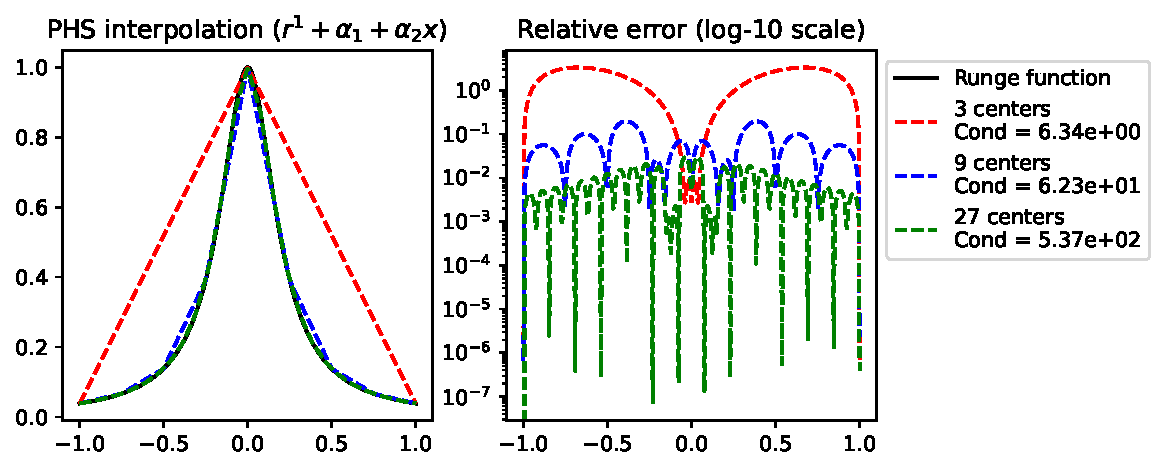
\includegraphics[width=\textwidth]{imagenes/phs_interpolation/runge_phs_r1_deg1.pdf}
  \caption{Left-hand side: PHS interpolation ($r^1$ alongside a linear polynomial). Right-hand side: relative interpolation error.}
  \label{fig:phs-runge-phenomenon-deg-1-discussion}
\end{figure}

\begin{figure}[ht]
  \centering
  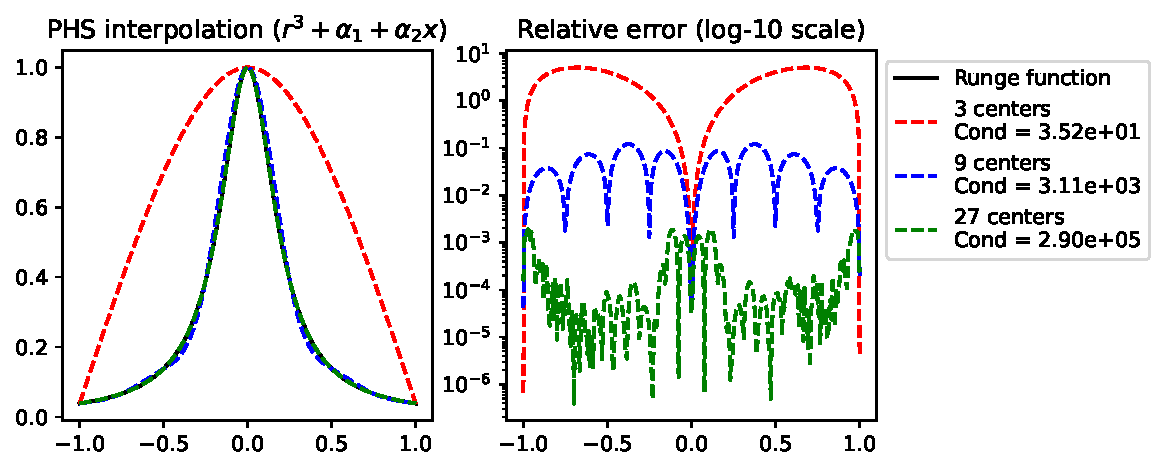
\includegraphics[width=\textwidth]{imagenes/phs_interpolation/runge_phs_r3_deg1.pdf}
  \caption{Left-hand side: PHS interpolation ($r^3$ alongside a linear polynomial). Right-hand side: relative interpolation error.}
  \label{fig:phs-runge-phenomenon-deg-3-discussion}
\end{figure}

Furthermore, Figures \ref{fig:phs-runge-phenomenon-deg-5} and \ref{fig:phs-runge-phenomenon-deg-7} of the Appendix show that, for $r^5$ and $r^7$, oscillations start appearing when using only 9 equispaced centers. Moreover, the condition numbers start increasing up until the results obtained are completely unreliable.

Another such example of interest is \textbf{Gibbs' phenomenon}\footnote{The following images can be easily derived from the relevant \href{https://github.com/heqro/tfm-experiments/blob/main/introductory_notebooks/rbf_interpolation/gibbs_rbf_and_phs.ipynb}{Gibbs interpolation notebook}.}. Often described in the context of Fourier expansions of piecewise continuously differentiable functions, it establishes that oscillations are bound to occur near such points of non-differentiability (or even jump discontinuity).
Although our techniques do not involve Fourier analysis, the nature of the interpolators we chose (as well as the previous experimentation on Runge's phenomenon) dictate that a similar situation is bound to happen in our framework.

We first consider $x \mapsto \arctan{20x}$, which we promptly depict in Figure \ref{fig:arctan-with-points} for $n=9, 30$ equispaced points. We use as interpolators a polyharmonic spline of the form $\phi(r) = r^3+\alpha_0+\alpha_1 x$ and a Gaussian kernel with shape parameter $\varepsilon=5$.

\begin{figure}[ht]
  \centering
  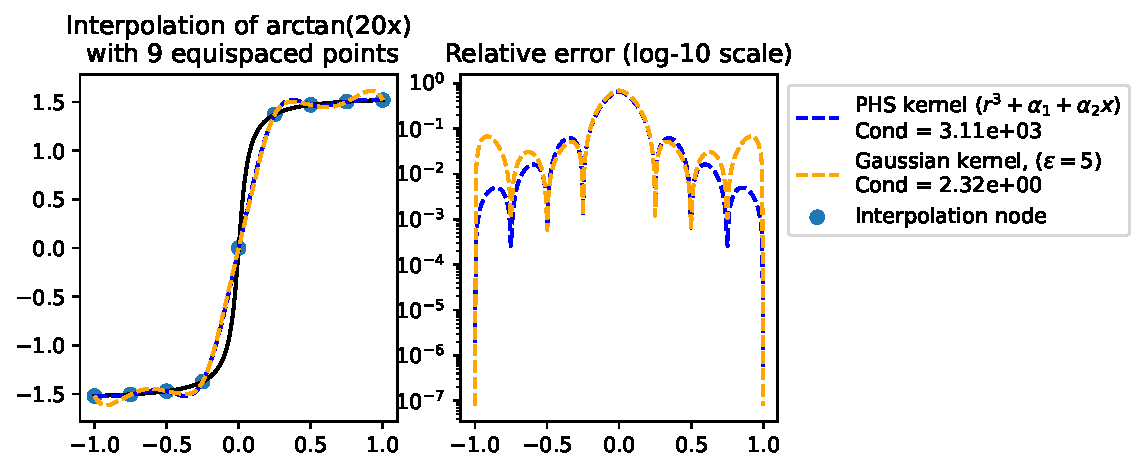
\includegraphics[width=\textwidth]{imagenes/experiments/1d/intro/arctan-with-9-pts.pdf}
  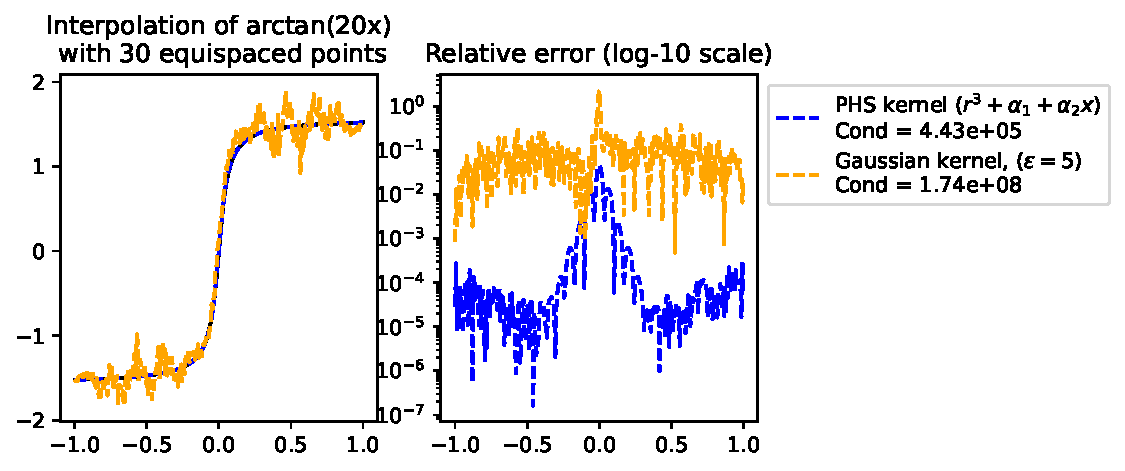
\includegraphics[width=\textwidth]{imagenes/experiments/1d/intro/arctan-with-30-pts.pdf}
  \caption{Top image: interpolation of $\arctan{20x}$ with 9 equispaced points. Bottom image: interpolation of $\arctan{20x}$ with 30 equispaced points. }
  \label{fig:arctan-with-points}
\end{figure}

Strictly speaking, this function we first have considered is not exhibiting the Gibbs' phenomenon as we have defined it. Indeed, for a small sample of points, oscillations are evidently bound to occur as the distance between two consecutive interpolation points is too large for the interpolator. For a larger sample of points, however, oscillations start up by the hand of the ill-conditioning of both interpolation matrices.

\begin{figure}[ht]
  \centering
  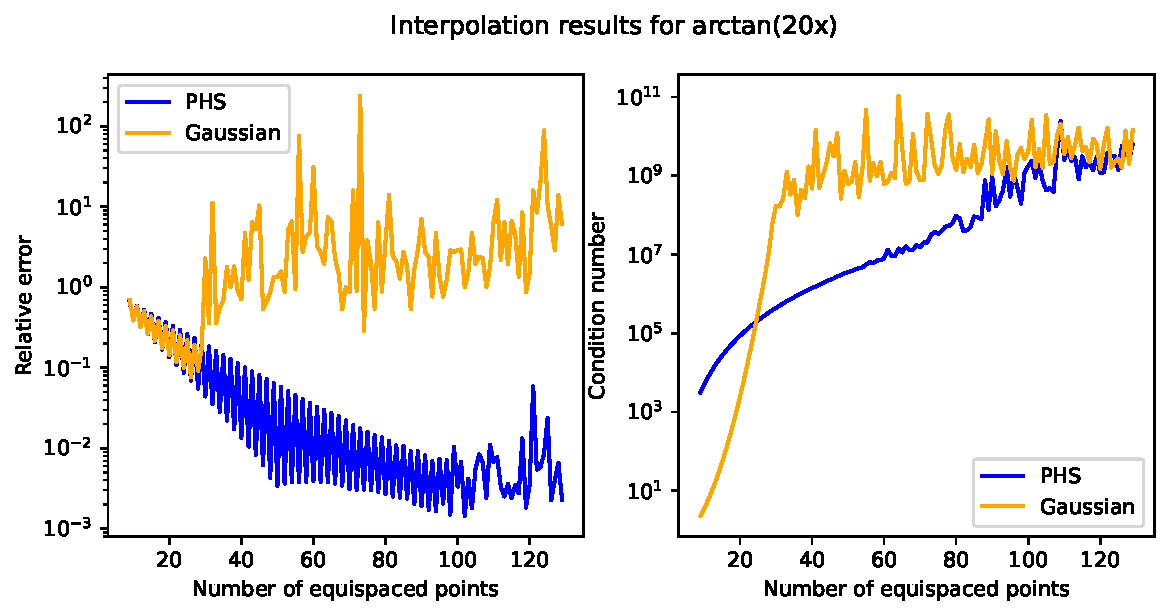
\includegraphics[width=.8\textwidth]{imagenes/experiments/1d/intro/arctan20x-interpolation-curves.pdf}
  \caption{Left-hand side: relative error in the interpolation of $\arctan{20x}$. Right-hand side: condition number of the interpolation matrix.}
  \label{fig:arctan-with-curves}
\end{figure}

Furthermore, Figure \ref{fig:arctan-with-curves} shows that the shape parameter for the Gaussian kernel is not capable of providing any reliable information past the 30 interpolation points, which coincides with the point after which oscillations start showing up for its condition number. On the other hand, the prescribed PHS kernel is capable of providing further accuracy with oscillations in the relative error only showing up past the hundred interpolation points.

In conclusion, even though this particular function does not exhibit Gibbs' phenomenon, it still is an interesting case study for analyzing oscillatory behavior in the Gaussian kernel. Moreover, it is a particular example where this kernel equipped with the proposed shape parameter can only provide a maximum of a digit of accuracy, which highlights again the difficulty of choosing a suitable shape parameter, and how ``one-fits-all'' parameters are unlikely for a varied enough sample of functions.

Gibbs' phenomenon shows up for increasingly larger coefficients of $x$ in $\arctan(20x)$. More specifically, by considering $x\mapsto \arctan(\alpha x)$ for $\alpha \to \infty$ we recover a scaled version of the sign function. Graphs in Figure \ref{fig:sign-with-20-pts} show that the oscillations occur most notably close to the jump due to the change in sign.

\begin{figure}[ht]
  \centering
  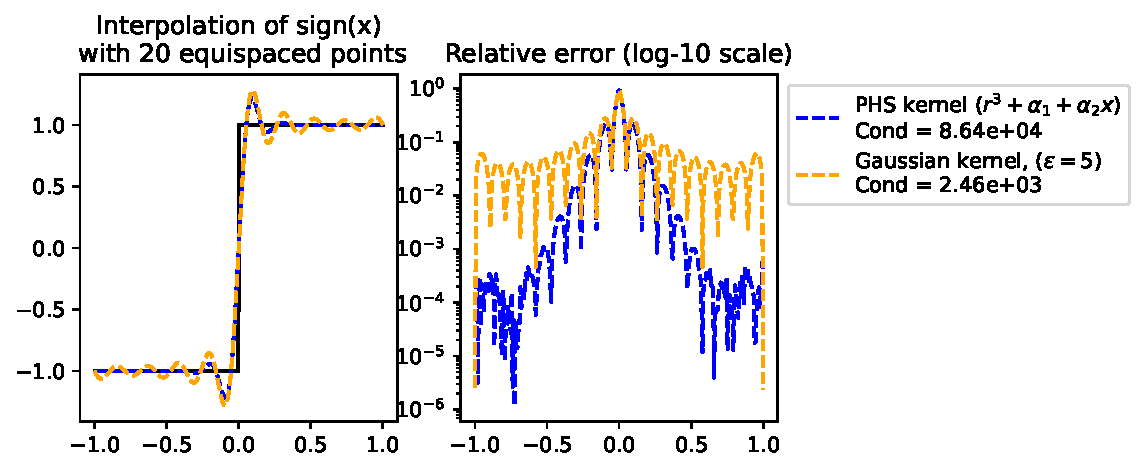
\includegraphics[width=\textwidth]{imagenes/experiments/1d/intro/sign-with-20-pts.pdf}
  \caption{Left-hand side: results of the interpolation of the sign function with 20 equispaced points. Right-hand side: relative error in logarithmic scale.}
  \label{fig:sign-with-20-pts}
\end{figure}

Figure \ref{fig:sign-with-curves} shows a poorer version of the situation shown in previously-analyzed Figure \ref{fig:arctan-with-curves}: even though the number of points where the condition number of the matrices prove to be too large for our problem are similar, neither of the two methods are capable of reducing the $L^\infty-$norm to provide any digit of accuracy in the worst case scenario.

\begin{figure}[ht]
  \centering
  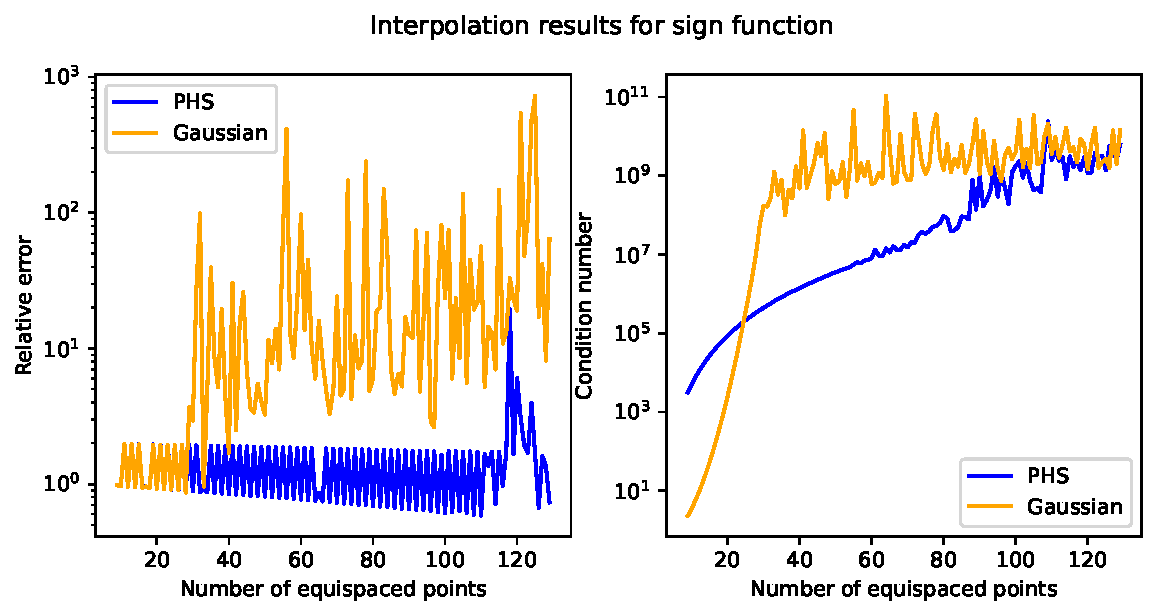
\includegraphics[width=.8\textwidth]{imagenes/experiments/1d/intro/sign-interpolation-curves.pdf}
  \caption{Left-hand side: relative error in the interpolation of the sign function. Right-hand side: condition number for the corresponding interpolation matrix.}
  \label{fig:sign-with-curves}
\end{figure}



\chapter{Experimentation}

\section{Hardware information}

All the experimentation featured in the following has been carried out in a server
kindly provided by my advisors.

\begin{table}[h]
  \begin{tabular}{|l|l|}
    \hline
    CPU & $\times 39$ Intel{\textregistered} Xeon{\textregistered} Silver
    4210R @ 2.40 GHz                                                      \\
    \hline
    GPU & NVIDIA RTX A6000 (49140 MiB)                                    \\
    \hline
    RAM & 251 Gi                                                          \\
    \hline
    OS  & Ubuntu 22.04.1 (Kernel 6.5.0-14)                                \\
    \hline
  \end{tabular}
  \caption{Description of the hardware used for experiments and development.}
  \label{tb:hardware-machinery}
\end{table}

\section{Interpolation}
\section*{Preliminary experimentation}

The methodology for solving Problem \ref{interpolationproblemstatement} using an RBF interpolator can be expressed in terms of a two-step process: the first step is explicitly locating the RBF centers and (if applicable) setting the value of the shape parameter $\varepsilon$. The second step involves computing the values of $\lambda$ as in \eqref{eqn-p-is-a-linear-combination-of-rbfs}, which ultimately leads to solve \eqref{eqn-linear-system-equations-rbf}. We refer to this methodology in the following as classic.

Alternatively to this methodology, we propose to let the centers as well as the shape parameters\footnote{We remark that we are now speaking in plural.} be found following an \textbf{unsupervised learning} strategy, whereby the training points will not only dictate the values of $\lambda$ as in \eqref{eqn-linear-system-equations-rbf}, but also the position of the RBF centers as well as the value of the shape parameters.
Therefore, it is interesting to compare the performance of this alternative methodology against the classic one, especially in their treatment of the oscillation
issues (Runge and Gibbs phenomena) we have previously observed. We will analyze
three different functions:
\begin{itemize}
  \item $1 / (1 + 25 x^2)$, which we may refer to as the Runge function or as \texttt{runge\_function}.

  \item $\tmop{arc} \tan (20 x)$, which we may refer to as the Gibbs
        function or as \texttt{gibbs\_function}.

  \item The sign function, which exhibits a behavior similar to that of the
        Gibbs function, but worse-posed from a mathematical perspective (for
        instance, non-differentiability appears). We may refer to it as \texttt{torch\_sign}.
\end{itemize}

We will also consider some additional functions which, despite exhibiting some
oscillations in their graph, we have preliminarily seen them not to pose any
pathologies when interpolating unlike the former two. This allows to verify that
the proposed methods do indeed work on a ``better-posed'' setting. In
particular, we consider the ``control'' functions
\begin{itemize}
  \item $ \sin (x^2)$ for $x \in [0,
            3]$. We may refer to it as \texttt{sin\_higher\_oscillations}.%\footnote{Defined \href{https://github.com/heqro/tfm-experiments/blob/1a4d7f00a5ae097f62db9fa912a8253e43efe60c/modules/notable_functions.py\#L52}{here} in the repository. We may refer to it as , but it has been redefined to fit in the interval $[-1,1]$ to ease up the programming.}.

  \item$ \sin (\pi x^2)$ for $x \in [- 1, 1]$. We may refer to it as \texttt{sin\_pi\_x\_sq}.%\footnote{Defined \href{https://github.com/heqro/tfm-experiments/blob/1a4d7f00a5ae097f62db9fa912a8253e43efe60c/modules/notable_functions.py\#L48}{here} in the repository. We may refer to it as }.
\end{itemize}

\begin{figure}[ht]
  \centering
  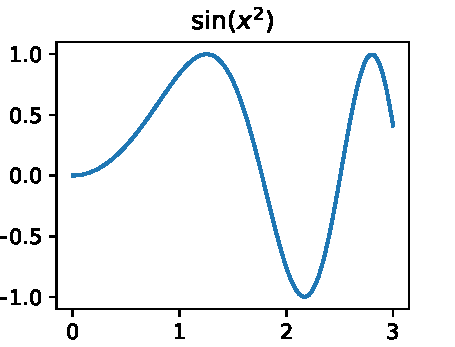
\includegraphics[width=.4\textwidth]{imagenes/experiments/1d/intro/sin_higher_oscillations.pdf}
  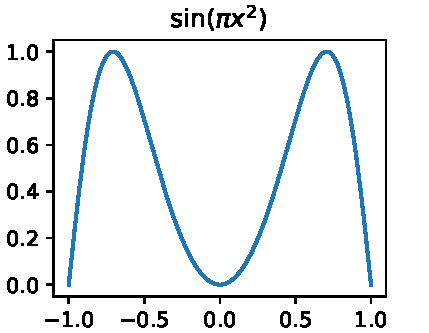
\includegraphics[width=.4\textwidth]{imagenes/experiments/1d/intro/sin_pi_x_sq.pdf}
  \caption{Left-hand side: $\sin (x^2)$ for $x \in [0,
        3]$. Right-hand side: $ \sin (\pi x^2)$ for $x \in [- 1, 1]$.}
  \label{fig:intro-control-functions}
\end{figure}

We use all these alternative terminologies for the functions in correspondence with their definition in the corresponding \href{https://github.com/heqro/tfm-experiments/blob/main/modules/notable_functions.py}{\texttt{notable\_functions}} module in the repository.

Each of these functions will be interpolated for under the Gaussian,
multiquadric and PHS kernels (in particular, $\phi(r)=r^3$ alongside a linear polynomial), which we may occasionally refer to as they are featured in the \href{https://github.com/heqro/tfm-experiments/blob/main/modules/notable_kernels.py}{\texttt{notable\_kernels}} module: \texttt{gaussian\_kernel}, \texttt{mq\_kernel\_sarra}, and \texttt{phs\_kernel}. Furthermore, a fourth kernel will be considered,
whereby the Gaussian kernel is to be accompanied by a polynomial of degree 1.


For each
``function-kernel-nodes'' triple, it is reasonable to ask the following
questions:

\begin{enumerate}[i]
  \item Fix the number of centers. Does the $L^{\infty}-$norm on the
        verification dataset decrease as we increase the number of training points?
        As the number of training points increases, is a larger number of iterations needed to achieve
        better results (in terms of the $L^{\infty}-$norm)?

  \item Repeat the previous step, but this time around by setting an increasingly larger
        number of centers.

  \item How do these experiments fare on the verification dataset against the
        classic methods?
\end{enumerate}

As an addition to these questions, we also wish to analyze if there are any performance gains by utilizing these
methods on Chebyshev nodes with respect to equispaced nodes.

Any individual experiment is then uniquely
characterized according to the parameters shown in Table \ref{tab:keys-table}. The last key of this table, ``add a polynomial'', corresponds to the possibility of complementing the Gaussian kernel with a polynomial of degree 1, the aforementioned fourth kernel. It has only been incorporated into the table for the sake of being exhaustive. It is also relevant to know that the type of nodes we choose will dictate the location of the training points as well as our centers'.

\begin{table}[h]
  \centering
  \begin{tabular}{|l|l|l|l|l|l|}
    \hline
    function & \# training points & \# centers & kernel & type of nodes &
    add a polynomial                                                      \\
    \hline
  \end{tabular}
  \caption{Table with experiment keys.}
  \label{tab:keys-table}
\end{table}

For the sake of allowing the experiments to be reproducible, we now comment on the parameters of the experiments we carry out with our method: \begin{itemize}
  \item We will seek to minimize the \textbf{mean-squared error} (MSE) between the interpolator applied to the evaluation point and the corresponding target training values.
  \item Learning rate: $10^{-2}$.
  \item Optimizer: Adam.
  \item Maximum number of iterations: 50000.
  \item The classic methods will be executed for $\varepsilon=5$ as shape parameter\footnote{As seen in Figure \ref{fig:xor-coefficients-conditioning} during the discussion of the \texttt{xor} binary operator, the choice of the shape parameter has an important impact on the conditioning of the matrix. Therefore, this parameter has been chosen to ensure that the interpolation problems are well-conditioned while preserving the quality of the results.}.
\end{itemize}

After having commented the experiments and terminology we will follow during the experiment, we can now address the questions we have posed. To this end, we first locate \hyperref[appendix-1d]{the corresponding Appendix} for the exhaustive relation of results of this experiment. Alongside our observations, we will include some of these results to avoid the reader from going back and forth in the text and thus facilitate the reading.

We first report the results involving the $L^\infty-$norm on the verification dataset
in the form of 3D heat maps, whereby the $x$ and $y$ coordinates correspond to the number of centers
and training points respectively, and the $z$ entry corresponds to the minimum across all iterations
of the logarithm of this norm.
We will also show during which iterations these values are achieved. This way, we can possibly tell if
we have ``stabilized'' to a solution without oscillations or if this may not be the case.


We start the report by assessing the impact of the last two experiment keys
of Table \ref{tab:keys-table}, namely the addition of a polynomial term and
the type of nodes we choose to work with, on the experiments with the proposed methodology as well as the classic methodology.

The \textbf{addition of a polynomial} term
does not have any significant impact on the $L^{\infty} -$norm. As a representative result of the experiments carried out under the proposed method, Figure \ref{fig:runge-gaussian-comparison-poly-equi} compares the $L^{\infty} -$norm of the interpolation of the Runge function under equispaced training points using a polynomial term (right-hand side) and not using it (left-hand side).

\begin{figure}[h]
  \begin{tabular}{cc}
    \multicolumn{2}{c}{{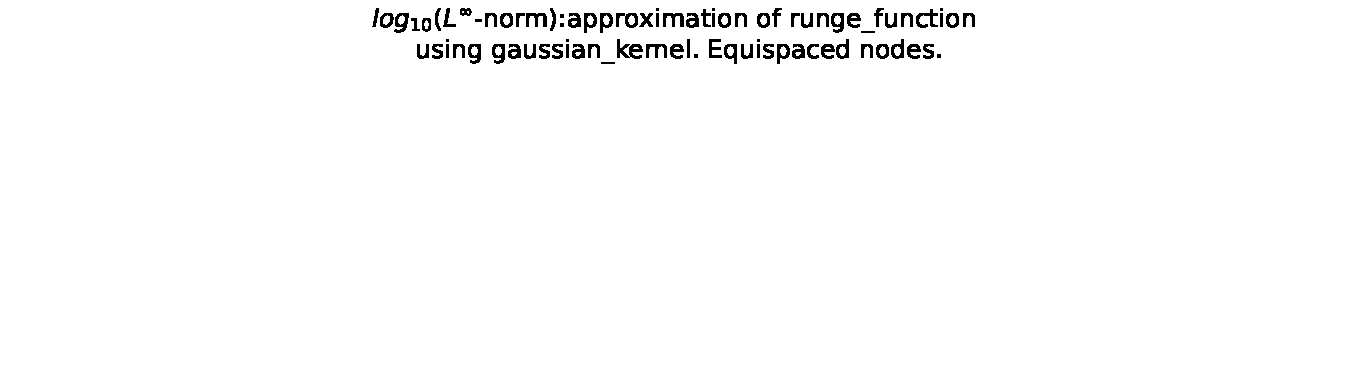
\includegraphics[width=\textwidth, trim={0 5.5cm 0 0},clip=true]
    {imagenes/experiments/1d/variational/linf_runge_function_gaussian_kernel_Equi_Poly_Title.pdf}}}                                                                                       \\
    {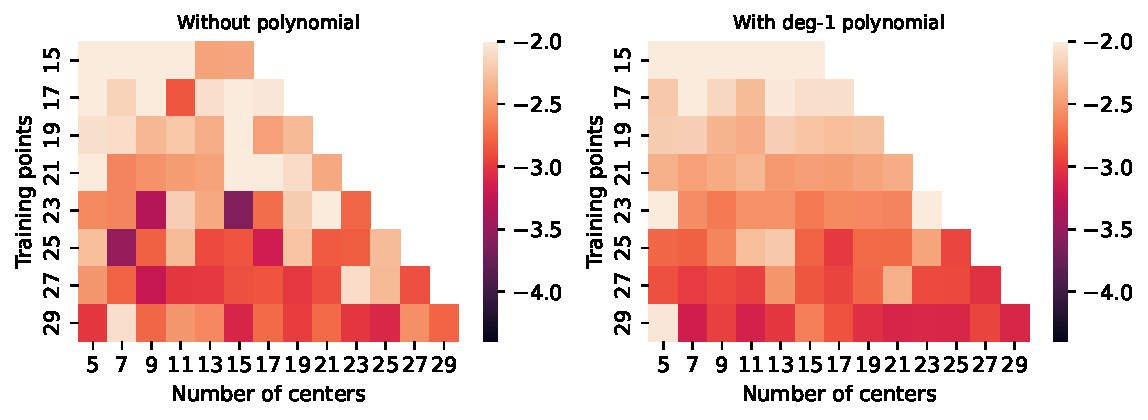
\includegraphics[height=.4\textwidth, trim={0 0 11.5cm 0},clip=true]
    {imagenes/experiments/1d/variational/linf_runge_function_gaussian_kernel_Equi_Poly_Comparison.pdf}}  &
     {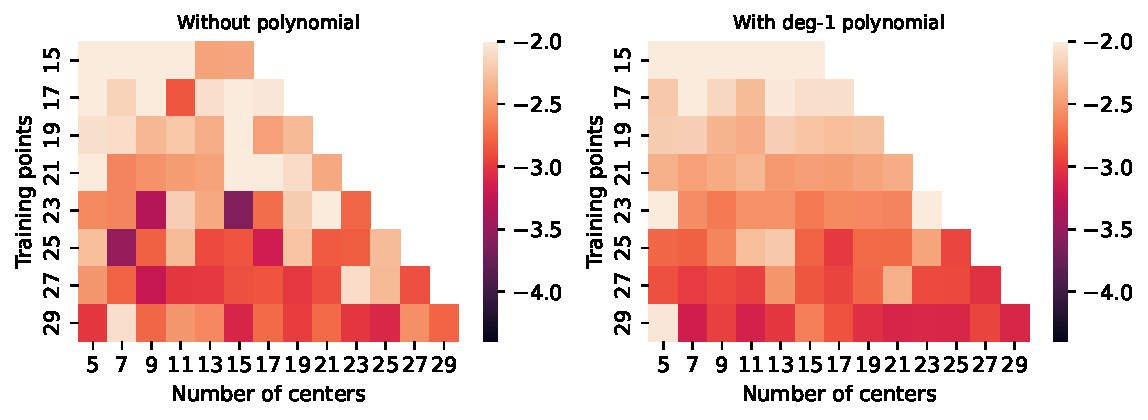
\includegraphics[height=.4\textwidth, trim={9.52cm 0 0 0},clip=true]{imagenes/experiments/1d/variational/linf_runge_function_gaussian_kernel_Equi_Poly_Comparison.pdf}} \\
  \end{tabular}
  \caption{Logarithm of the $L^\infty-$norm of the approximation of the Runge function with a Gaussian kernel using equispaced nodes, comparing the performance our method using no polynomial term (left-hand side) as well as a linear polynomial term (right-hand side).}
  \label{fig:runge-gaussian-comparison-poly-equi}
\end{figure}

There is no tendency on the classic methodology
that clearly favors the choice of a \textbf{set of training nodes} or the other. For instance,
Figure \ref{fig:runge-sarra-comparison-opt-points} shows that the choice of equispaced nodes may
be preferable for the particular case of the interpolation of the
Runge function with a multiquadric kernel: with 19 equispaced centers we may
guarantee around 3 digits of precision, whereas this happens with 29 centers
in a Chebyshev disposition.

\begin{figure}[h]
  \begin{tabular}{cc}
    \multicolumn{2}{c}{{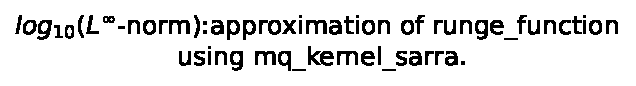
\includegraphics[width=.5\textwidth]
    {imagenes/experiments/1d/variational/linf_runge_function_mq_kernel_sarra_Points_Classic_Title.pdf}}}                                                                                       \\
    {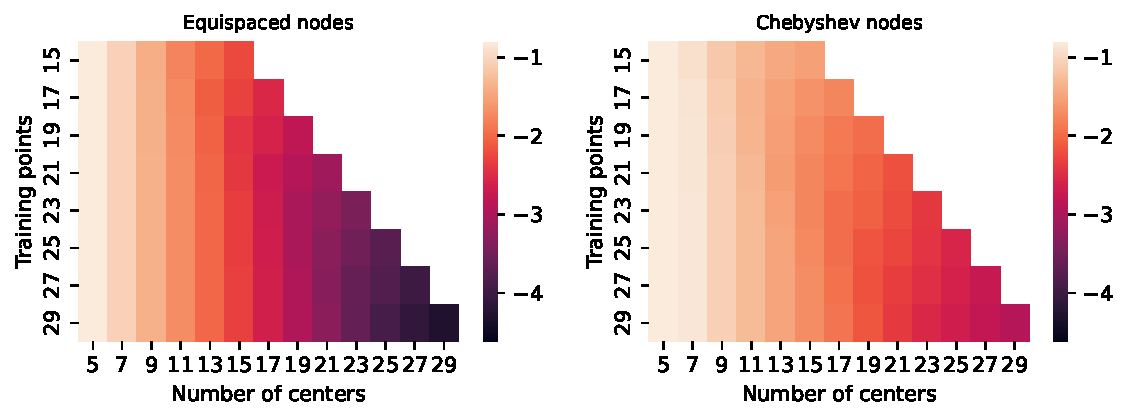
\includegraphics[height=.4\textwidth, trim={0 0 11.2cm 0},clip=true]
    {imagenes/experiments/1d/variational/linf_runge_function_mq_kernel_sarra_Points_Classic_Comparison.pdf}}  &
     {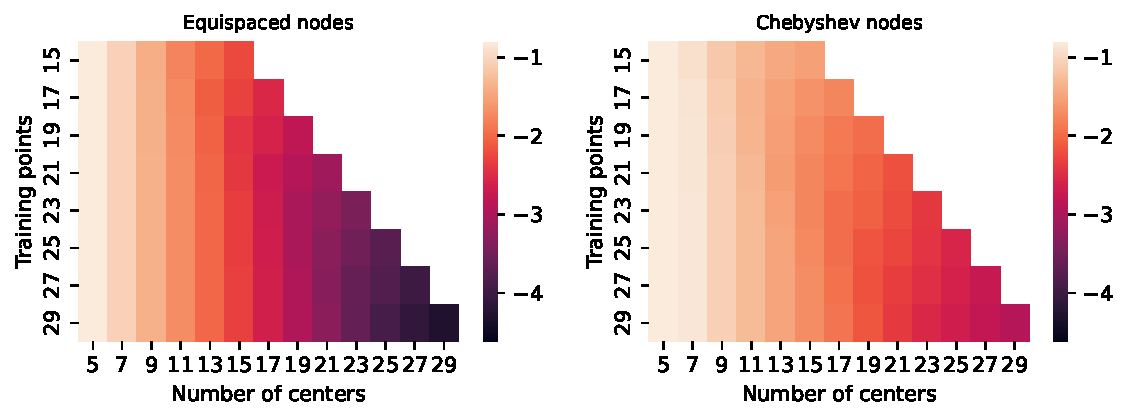
\includegraphics[height=.4\textwidth, trim={9.5cm 0 0 0},clip=true]{imagenes/experiments/1d/variational/linf_runge_function_mq_kernel_sarra_Points_Classic_Comparison.pdf}} \\
  \end{tabular}
  \caption{Logarithm of the $L^\infty-$norm of the approximation of the Runge function with the multiquadric kernel using equispaced nodes, comparing the performance of equispaced with Chebyshev nodes.}
  \label{fig:runge-sarra-comparison-opt-points}
\end{figure}

In other occasions, the situation is the opposite. Such is the case of the interpolation of
\texttt{sin\_higher\_oscillations} with the Gaussian (as well as multiquadric) kernel,
proportioning a digit of accuracy more than the equispaced layout as per
Figure \ref{fig:sin-higher-oscillations-gaussian-kernel-comparison-points-classic}.

\begin{figure}[h]
  \begin{tabular}{cc}
    \multicolumn{2}{c}{{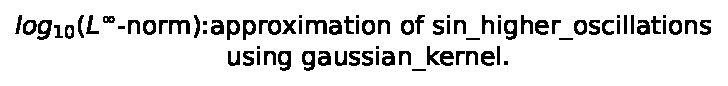
\includegraphics[width=.5\textwidth]
    {imagenes/experiments/1d/variational/linf_sin_higher_oscillations_gaussian_kernel_Points_Classic_Title.pdf}}}                                                                                       \\
    {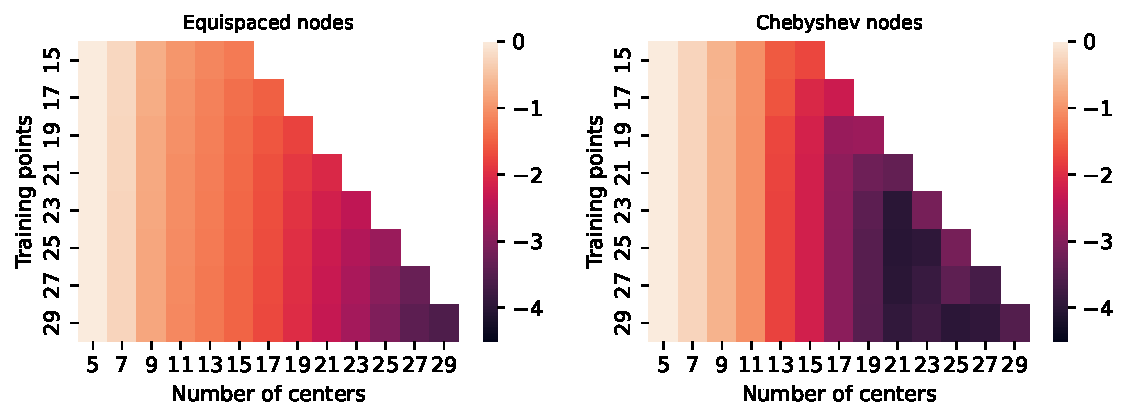
\includegraphics[height=.4\textwidth, trim={0 0 11.5cm 0},clip=true]
    {imagenes/experiments/1d/variational/linf_sin_higher_oscillations_gaussian_kernel_Points_Classic_Comparison.pdf}}  &
     {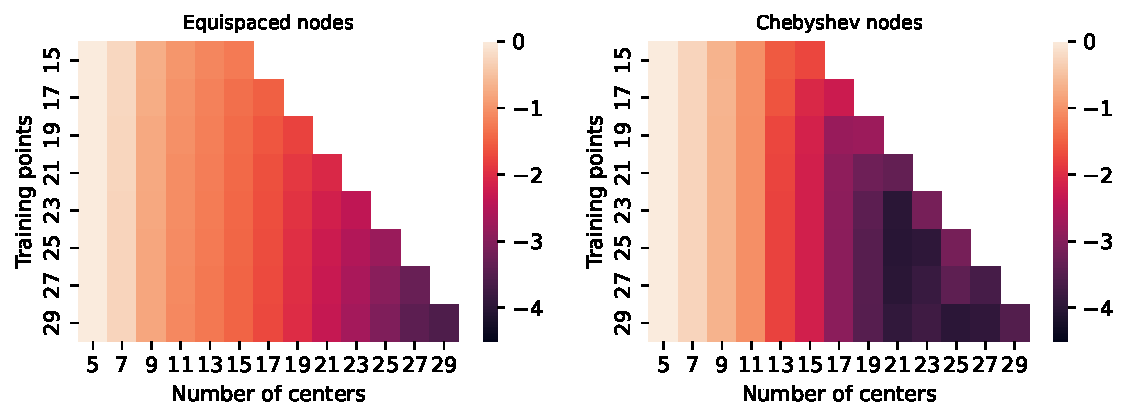
\includegraphics[height=.4\textwidth, trim={9.5cm 0 0 0},clip=true]{imagenes/experiments/1d/variational/linf_sin_higher_oscillations_gaussian_kernel_Points_Classic_Comparison.pdf}} \\
  \end{tabular}
  \caption{Logarithm of the $L^\infty-$norm of the approximation of the Runge function with a Gaussian kernel using equispaced nodes, comparing the performance our method using no polynomial term (left-hand side) as well as a linear polynomial term (right-hand side).}
  \label{fig:sin-higher-oscillations-gaussian-kernel-comparison-points-classic}
\end{figure}

There is no clear preference on either set of nodes under our methodology either. For instance, Figure \ref{fig:runge-function-gaussian-kernel-comparison-points-classic} and \ref{fig:gibbs-function-gaussian-kernel-comparison-points-classic} show an advantage in favor of the equispaced distribution of points when dealing with Runge's and Gibbs' phenomena, respectively.

\begin{figure}[h]
  \begin{tabular}{cc}
    \multicolumn{2}{c}{{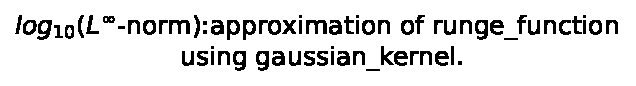
\includegraphics[width=.5\textwidth]
    {imagenes/experiments/1d/variational/linf_runge_function_gaussian_kernel_Points_Title.pdf}}}                                                                                       \\
    {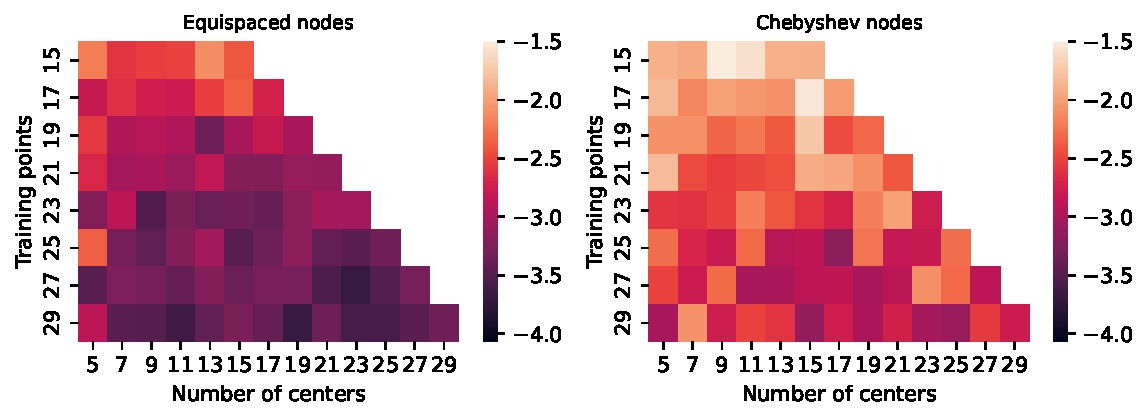
\includegraphics[height=.4\textwidth, trim={0 0 11.5cm 0},clip=true]
    {imagenes/experiments/1d/variational/linf_runge_function_gaussian_kernel_Points_Comparison.pdf}}  &
     {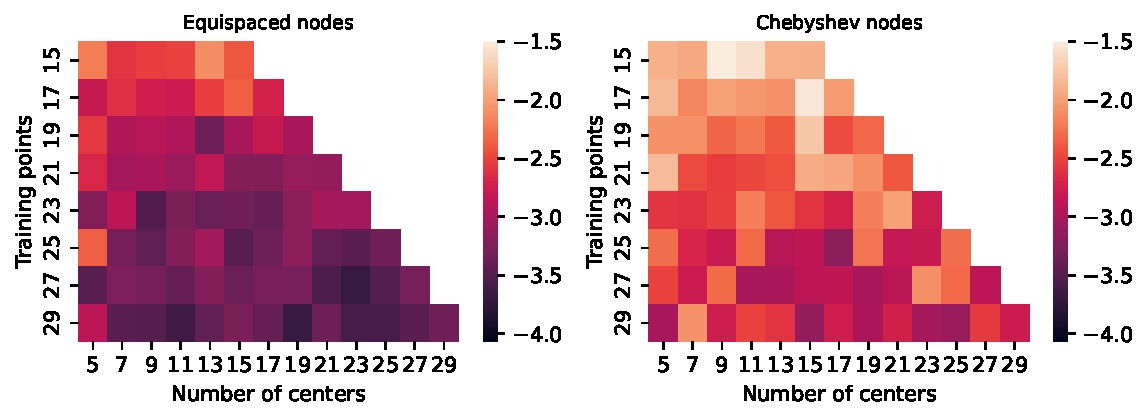
\includegraphics[height=.4\textwidth, trim={9.5cm 0 0 0},clip=true]{imagenes/experiments/1d/variational/linf_runge_function_gaussian_kernel_Points_Comparison.pdf}} \\
  \end{tabular}
  \caption{Logarithm of the $L^\infty-$norm of the approximation of the Runge function with a Gaussian kernel using equispaced nodes (left-hand side) and Chebyshev nodes (right-hand side).}
  \label{fig:runge-function-gaussian-kernel-comparison-points-classic}
\end{figure}

\begin{figure}[h]
  \begin{tabular}{cc}
    \multicolumn{2}{c}{{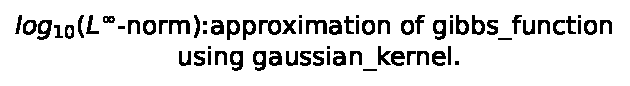
\includegraphics[width=.5\textwidth]
    {imagenes/experiments/1d/variational/linf_gibbs_function_gaussian_kernel_Points_Title.pdf}}}                                                                                       \\
    {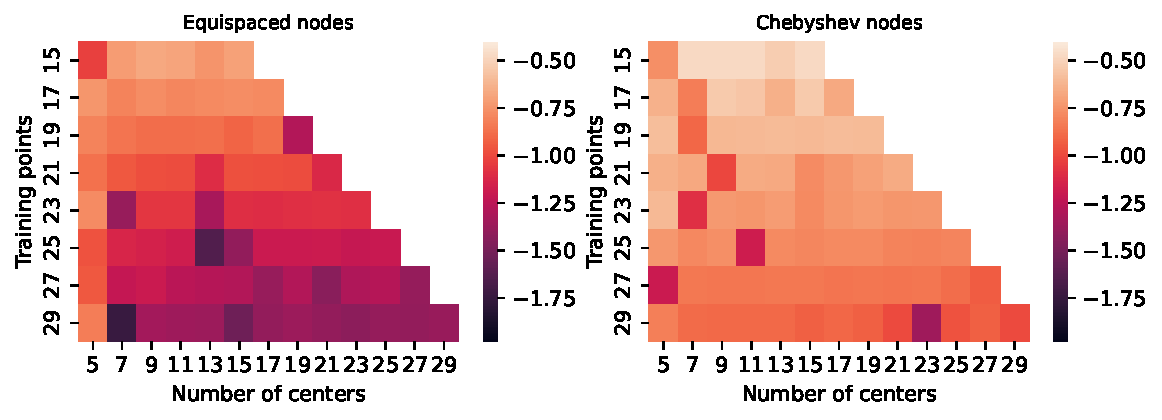
\includegraphics[height=.4\textwidth, trim={0 0 11.8cm 0},clip=true]
    {imagenes/experiments/1d/variational/linf_gibbs_function_gaussian_kernel_Points_Comparison.pdf}}  &
     {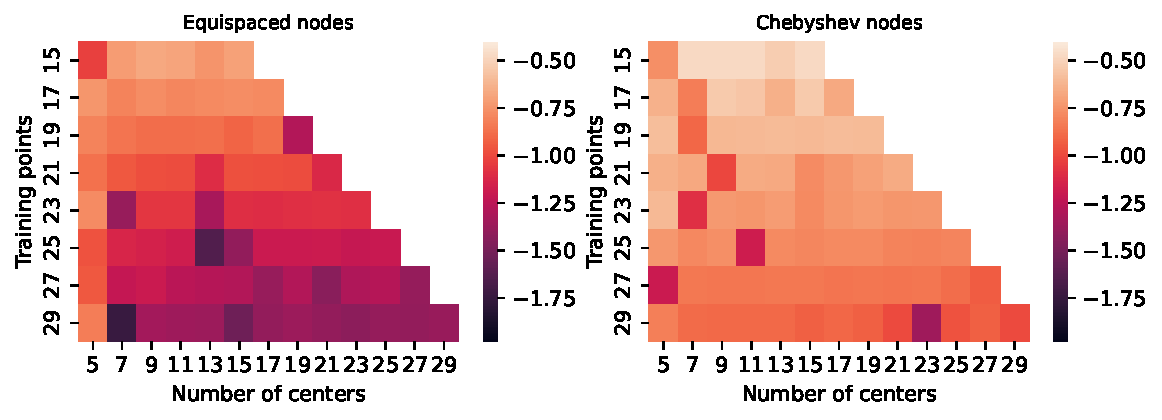
\includegraphics[height=.4\textwidth, trim={9.8cm 0 0 0},clip=true]{imagenes/experiments/1d/variational/linf_gibbs_function_gaussian_kernel_Points_Comparison.pdf}} \\
  \end{tabular}
  \caption{Logarithm of the $L^\infty-$norm of the approximation of the Gibbs function with a Gaussian kernel using equispaced nodes (left-hand side) and Chebyshev nodes (right-hand side).}
  \label{fig:gibbs-function-gaussian-kernel-comparison-points-classic}
\end{figure}


Conversely, Figure \ref{fig:sin-higher-oscillations-gaussian-kernel-comparison}, which depicts the heat map of the interpolation of the function \texttt{sin-higher-oscillations} with a Gaussian interpolator, shows that Chebyshev nodes allow for generally better results than with Equispaced nodes.

\begin{figure}[H]
  \begin{tabular}{cc}
    \multicolumn{2}{c}{{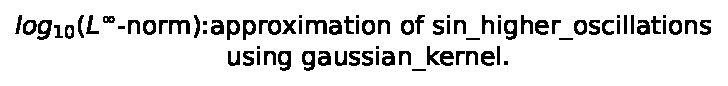
\includegraphics[width=.5\textwidth]
    {imagenes/experiments/1d/variational/linf_sin_higher_oscillations_gaussian_kernel_Points_Title.pdf}}}                                                                                       \\
    {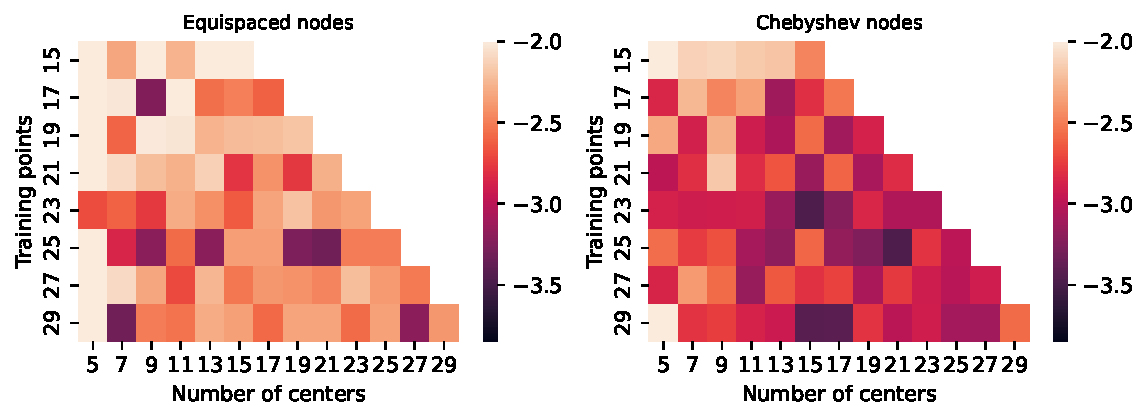
\includegraphics[height=.4\textwidth, trim={0 0 11.5cm 0},clip=true]
    {imagenes/experiments/1d/variational/linf_sin_higher_oscillations_gaussian_kernel_Points_Comparison.pdf}}  &
     {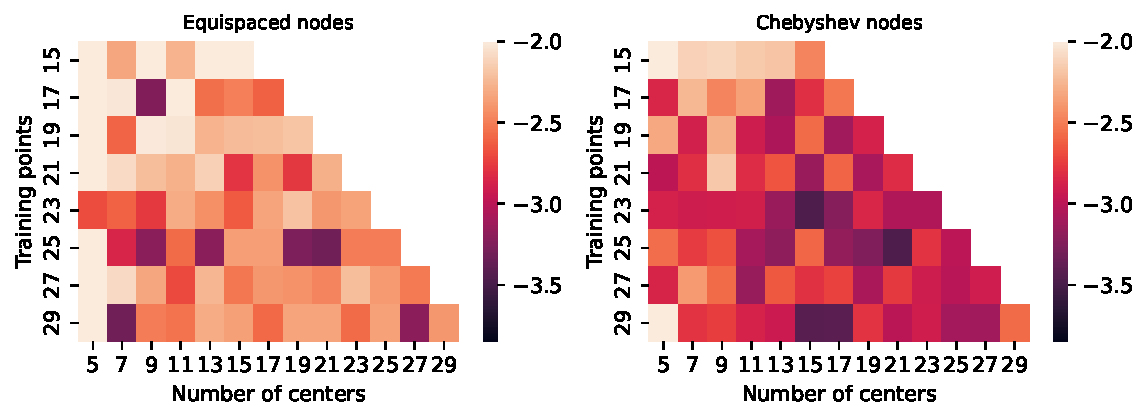
\includegraphics[height=.4\textwidth, trim={9.5cm 0 0 0},clip=true]{imagenes/experiments/1d/variational/linf_sin_higher_oscillations_gaussian_kernel_Points_Comparison.pdf}} \\
  \end{tabular}
  \caption{Logarithm of the $L^\infty-$norm of the approximation of the Runge function with a multiquadric kernel using equispaced nodes, comparing the performance our method using no polynomial term (left-hand side) as well as a linear polynomial term (right-hand side).}
  \label{fig:sin-higher-oscillations-gaussian-kernel-comparison}
\end{figure}

Therefore, it is not clear if any particular choice of training nodes is better. There is also no notable performance gain when incorporating a polynomial addend. For this reason, the remainder of the report defaults to commenting the simpler
scenario: that of equispaced points and disregarding the fourth kernel (Gaussian + polynomial term). We first address the results with the Gaussian and multiquadric kernels. Secondly, we discuss the results involving the PHS kernel.

Starting with the Runge function, our method reduces the
$L^{\infty} -$norm performs comparably to the classic method across the Gaussian and multiquadric kernels.
We first refer to Figure \ref{fig:runge-gaussian-comparison-equi-classic}, which shows a comparison on the $L^\infty-$norm for the Gaussian kernel. Notice that our method yields a minimum of two digits of accuracy across all tests. The classic method starts exhibiting this performance level when supplied with 13
centers or more, visually yielding the same accuracy irrespectively of the number of training points. Our method is capable of making the most of the training points, possibly yielding three digits of accuracy with just 5 centers and 27 training points. %This is a noticeable difference with the classic method, which is more sensitive to the number of centers than the training points.


\begin{figure}[H]
  \begin{tabular}{cc}
    \multicolumn{2}{c}{{\includegraphics[width=.5\textwidth]
    {imagenes/experiments/1d/variational/linf_runge_function_gaussian_kernel_Equi_Classic_Title.pdf}}}                                                                                       \\
    {\includegraphics[height=.4\textwidth, trim={0 0 11.5cm 0},clip=true]
    {imagenes/experiments/1d/variational/linf_runge_function_gaussian_kernel_Equi_Classic_Comparison.pdf}}  &
     {\includegraphics[height=.4\textwidth, trim={9.5cm 0 0 0},clip=true]{imagenes/experiments/1d/variational/linf_runge_function_gaussian_kernel_Equi_Classic_Comparison.pdf}} \\
  \end{tabular}
  \caption{Logarithm of the $L^\infty-$norm of the approximation of the Runge function with a Gaussian kernel using equispaced nodes, comparing the performance our method using no polynomial term (left-hand side) as well as a linear polynomial term (right-hand side).}
  \label{fig:runge-gaussian-comparison-equi-classic}
\end{figure}

This tendency is also present in Figure \ref{fig:runge-mq-sarra-kernel-comparison-equi-classic}, which compares the performance of the multiquadric kernel: %on the same data set-ups: the 
results show that our method is capable of not exhibiting oscillations even when trained with a small amount of training points and centers.
However, the figure shows that the multiquadric kernel (under the classic method) is capable of giving up to four digits of accuracy when solving for 29 training points and 29 centers, which our method is not capable of achieving.

\begin{figure}[h]
  \begin{tabular}{cc}
    \multicolumn{2}{c}{{\includegraphics[width=.5\textwidth]
    {imagenes/experiments/1d/variational/linf_runge_function_mq_kernel_sarra_Equi_Classic_Title.pdf}}}                                                                                       \\
    {\includegraphics[height=.4\textwidth, trim={0 0 11.5cm 0},clip=true]
    {imagenes/experiments/1d/variational/linf_runge_function_mq_kernel_sarra_Equi_Classic_Comparison.pdf}}  &
     {\includegraphics[height=.4\textwidth, trim={9.5cm 0 0 0},clip=true]{imagenes/experiments/1d/variational/linf_runge_function_gaussian_kernel_Equi_Classic_Comparison.pdf}} \\
  \end{tabular}
  \caption{Logarithm of the $L^\infty-$norm of the approximation of the Runge function with a multiquadric kernel using equispaced nodes, comparing the performance our method (left-hand side) against the classic one (right-hand side).}
  \label{fig:runge-mq-sarra-kernel-comparison-equi-classic}
\end{figure}

For the Gibbs phenomenon, we may just refer to the experiments carried out
with the Gaussian kernel (see Figure
\ref{fig:gibbs-gaussian-kernel-comparison-classic}), because the same
observations hold for the multiquadric kernel as well. For the
classic methodology, it suffices to note that we need to consider
21 centers just to be able to remove oscillations to the first digit of
accuracy. However, a number of centers larger than 7 and a number of training
points larger than 23 is sufficient to give this first digit of accuracy.

\begin{figure}[h]
  \begin{tabular}{cc}
    \multicolumn{2}{c}{{\includegraphics[width=.5\textwidth]
    {imagenes/experiments/1d/variational/linf_gibbs_function_gaussian_kernel_Methods_Title.pdf}}}                                                                                       \\
    {\includegraphics[height=.4\textwidth, trim={0 0 11.5cm 0},clip=true]
    {imagenes/experiments/1d/variational/linf_gibbs_function_gaussian_kernel_Methods_Comparison.pdf}}  &
     {\includegraphics[height=.4\textwidth, trim={9.5cm 0 0 0},clip=true]{imagenes/experiments/1d/variational/linf_gibbs_function_gaussian_kernel_Methods_Comparison.pdf}} \\
  \end{tabular}
  \caption{Logarithm of the $L^\infty-$norm of the approximation of the Gibbs function with a Gaussian kernel using equispaced nodes, comparing the performance our method (left-hand side) against the classic one (right-hand side).}
  \label{fig:gibbs-gaussian-kernel-comparison-classic}
\end{figure}

Like
in the case of the Runge phenomenon, the classic methodology improves
the results as the number of centers increases, whereas our methodology
produces better results as the number of training points increases.
Notwithstanding, neither of the two methods are not able to decisively reduce the oscillations with the given amounts of centers and training points, that is, they can only provide in the best case scenario a digit of accuracy under the tests we carried out.

We now address the results of our experiments on the function named for convenience \texttt{sin\_higher\_oscillations}. As for the Gaussian kernel (see Figure \ref{fig:sin-higher-oscillations-gaussian-kernel-comparison-methods}), we observe that our method is capable of providing two digits of accuracy in almost every experiment configuration, bar the ones involving 5 centers and 15 and 19 training points. In a similar vein to the previous experiments, we observe that there are indeed dispositions of centers that are able to minimize oscillations providing three digits of accuracy (compare, for instance, the results of both methods involving 17 training points and 9 centers).

\begin{figure}[h]
  \begin{tabular}{cc}
    \multicolumn{2}{c}{{\includegraphics[width=.5\textwidth]
    {imagenes/experiments/1d/variational/linf_sin_higher_oscillations_gaussian_kernel_Methods_Title.pdf}}}                                                                                       \\
    {\includegraphics[height=.4\textwidth, trim={0 0 11.5cm 0},clip=true]
    {imagenes/experiments/1d/variational/linf_sin_higher_oscillations_gaussian_kernel_Methods_Comparison.pdf}}  &
     {\includegraphics[height=.4\textwidth, trim={9.5cm 0 0 0},clip=true]{imagenes/experiments/1d/variational/linf_sin_higher_oscillations_gaussian_kernel_Methods_Comparison.pdf}} \\
  \end{tabular}
  \caption{Logarithm of the $L^\infty-$norm of the approximation of \texttt{sin\_higher\_oscillations} with a Gaussian kernel using equispaced nodes, comparing the performance our method (left-hand side) against the classic one (right-hand side).}
  \label{fig:sin-higher-oscillations-gaussian-kernel-comparison-methods}
\end{figure}

Much like the other experiments involving the multiquadric kernel, we observe that its performance is not as impressive as that of the Gaussian kernel, providing a digit of accuracy less than the latter. Such is the case again for \texttt{sin-higher-oscillations}, depicted in Figure \ref{fig:sin-higher-oscillations-mq-kernel-sarra-comparison-methods}. The addition of more centers does not have a noticeable effect on our method as well as on the classic method. %The former, however, is on a tendency to improve the results as more training points are provided (check, for instance, the 11th and 13th columns), whereas the latter seems not to improve performance past the addition of 13 centers. 
Providing more training points does not noticeably improve the results for the classic method, in coherence with the previous results we have observed.

\begin{figure}[h]
  \begin{tabular}{cc}
    \multicolumn{2}{c}{{\includegraphics[width=.5\textwidth]
    {imagenes/experiments/1d/variational/linf_sin_higher_oscillations_mq_kernel_sarra_Methods_Title.pdf}}}                                                                                       \\
    {\includegraphics[height=.4\textwidth, trim={0 0 11.5cm 0},clip=true]
    {imagenes/experiments/1d/variational/linf_sin_higher_oscillations_mq_kernel_sarra_Methods_Comparison.pdf}}  &
     {\includegraphics[height=.4\textwidth, trim={9.5cm 0 0 0},clip=true]{imagenes/experiments/1d/variational/linf_sin_higher_oscillations_mq_kernel_sarra_Methods_Comparison.pdf}} \\
  \end{tabular}
  \caption{Logarithm of the $L^\infty-$norm of the approximation of \texttt{sin\_higher\_oscillations} with a multiquadric kernel using equispaced nodes, comparing the performance our method (left-hand side) against the classic one (right-hand side).}
  \label{fig:sin-higher-oscillations-mq-kernel-sarra-comparison-methods}
\end{figure}

Now, we turn to \texttt{sin\_pi\_x\_sq}. We first refer to Figure \ref{fig:sin-pi-x-sq-gaussian-kernel-comparison-methods} for a comparison of the performance of both methods using the Gaussian kernel. We observe that, avoiding the case where we consider 5 centers, all other configurations are able to yield a minimum of two digits of accuracy. For this to happen with the classic method, we require the consideration of 21 centers.

\begin{figure}[h]
  \begin{tabular}{cc}
    \multicolumn{2}{c}{{\includegraphics[width=.5\textwidth]
    {imagenes/experiments/1d/variational/linf_sin_pi_x_sq_gaussian_kernel_Methods_Title.pdf}}}                                                                                       \\
    {\includegraphics[height=.4\textwidth, trim={0 0 11.5cm 0},clip=true]
    {imagenes/experiments/1d/variational/linf_sin_pi_x_sq_gaussian_kernel_Methods_Comparison.pdf}}  &
     {\includegraphics[height=.4\textwidth, trim={9.5cm 0 0 0},clip=true]{imagenes/experiments/1d/variational/linf_sin_pi_x_sq_gaussian_kernel_Methods_Comparison.pdf}} \\
  \end{tabular}
  \caption{Logarithm of the $L^\infty-$norm of the approximation of \texttt{sin\_pi\_x\_sq} with a Gaussian kernel using equispaced nodes, comparing the performance our method (left-hand side) against the classic one (right-hand side).}
  \label{fig:sin-pi-x-sq-gaussian-kernel-comparison-methods}
\end{figure}


We close this section of the report by turning to the case of the PHS interpolator. Figure \ref{fig:runge-function-phs-kernel-comparison-methods} shows a representative experiment that compares our methodology with the classic one. Our method is close to providing a single digit of accuracy in the $L^\infty-$norm, whereas the other is capable of providing a digit of accuracy just by the consideration of 7 centers, reaching around 3 digits of accuracy with just 15 centers. Unlike the other kernels we have considered, the PHS kernel does not significantly improve the results facing larger training points nor centers, which leads one to ponder if our iterative methodology may be ``stuck'' on a local minimum for this particular kernel.

\begin{figure}[h]
  \begin{tabular}{cc}
    \multicolumn{2}{c}{{\includegraphics[width=.5\textwidth]
    {imagenes/experiments/1d/variational/linf_runge_function_phs_kernel_Methods_Title.pdf}}}                                                                                       \\
    {\includegraphics[height=.4\textwidth, trim={0 0 11.5cm 0},clip=true]
    {imagenes/experiments/1d/variational/linf_runge_function_phs_kernel_Methods_Comparison.pdf}}  &
     {\includegraphics[height=.4\textwidth, trim={9.5cm 0 0 0},clip=true]{imagenes/experiments/1d/variational/linf_runge_function_phs_kernel_Methods_Comparison.pdf}} \\
  \end{tabular}
  \caption{Logarithm of the $L^\infty-$norm of the approximation of the Runge function with a PHS kernel using equispaced nodes, comparing the performance our method (left-hand side) against the classic one (right-hand side).}
  \label{fig:runge-function-phs-kernel-comparison-methods}
\end{figure}

A reasonable concern is the following: the results we have commented on are the comparison of the classic methodology against the iterations that minimized the $L^\infty-$norm on the verification dataset. If these optimal iterations are close to the maximum of iterations we have considered (recall that it is 50000), this indicates that our method ``converges'' to a solution which reduces the oscillations.

Other verification methods could have been considered, for instance:
\begin{enumerate}
  \item The ratio of the $L^\infty-$norms between the last and best iterations. Because we trained using the Adam optimizer, which considers ``jumps'' every so often to avoid converging to local minima, this ratio does not yield useful information, for any such ``jumps'' could have occurred close to the last iterations, which could lead us into the wrong direction.
  \item Refining the previous method, this time around inspecting the $L^\infty-$norm values iteration after iteration for every experiment, to verify if the few last thousands of iterations are reasonably close in value to the best iteration. Whereas this is indeed a sound strategy, it does not scale for the amount of experiments we have carried out.
        % It is worth considering, however, for specific experiments. \label{option-method}
\end{enumerate}

We start by calling up on the experiments involving the multiquadric kernel. Figure \ref{fig:epochs-sarra-kernel-report} shows the ratio of the best epoch to the number of total epochs for the interpolation of the Runge function with equispaced points. We can observe that, except for some outliers, the best iteration in terms of the $L^\infty-$norm on the verification dataset happens ``close'' to the maximum of iterations. This indicates that the multiquadric kernel does not only reduce oscillations, but that this reduction can be thought of as the ``stationary''\footnote{Because we work with the Adam optimizer, there is no (strictly speaking) a stationary regime. We mean that the long-term behavior of our interpolator is to minimize the oscillations, if we disregard the iterations where the optimizer tries to consider a different set of parameters.} regime of our iterative process.

\begin{figure}[ht]
  \centering
  \includegraphics[width=.49\textwidth]{imagenes/experiments/1d/variational_epochs/runge_function-Kmq_kernel_sarra-Equi-epochs.pdf}
  \caption{Ratio of the best epoch in the sense of the $L^\infty-$norm over the maximum number of epochs, for the interpolation of the Runge function with a multiquadric kernel and equispaced nodes.}
  \label{fig:epochs-sarra-kernel-report}
\end{figure}

Figure \ref{fig:epochs-gaussian-kernel-report} paints a different picture for the case of the Gaussian kernel. Indeed, the left-hand side shows that, about two thirds of the times, the iteration that minimizes the $L^\infty-$norm takes place close to the foreseen maximum of iterations. However, the right-hand side of this figure shows that it does not manage to cause the same impression for the Gibbs phenomenon. Similar conclusions can be drawn for the interpolation of the other functions we have considered.

\begin{figure}[h]
  \begin{tabular}{cc}
    \multicolumn{2}{c}{{\includegraphics[width=.5\textwidth]
    {imagenes/experiments/1d/variational/best_epochs_comparison_gaussian_kernel_Title.pdf}}}                                                                                       \\
    {\includegraphics[height=.4\textwidth, trim={0 0 11.5cm 0},clip=true]
    {imagenes/experiments/1d/variational/best_epochs_comparison_gaussian_kernel.pdf}}  &
     {\includegraphics[height=.4\textwidth, trim={9.5cm 0 0 0},clip=true]{imagenes/experiments/1d/variational/best_epochs_comparison_gaussian_kernel.pdf}} \\
  \end{tabular}
  \caption{Left-hand side: epochs ratio for the interpolation of the Runge function. Right-hand side: epochs ratio for the interpolation of the Gibbs function. In both images, interpolation has been carried out with the Gaussian kernel.}
  \label{fig:epochs-gaussian-kernel-report}
\end{figure}

To close the report, we turn to elaborate on why the results may be poor for the \textbf{PHS kernel}.
The left-hand side of Figure \ref{fig:epochs-runge-phs-show} depicts the interpolation of the Runge function with a PHS kernel and equispaced points, indicating that the best iteration in the $L^\infty-$norm for the PHS kernel interpolation is close to the last iteration we consider. This is actually the case for every experiment involving this kernel.


The right-hand side of this same figure depicts the distribution of the centers at the last iteration of our process, under 15 and 17 training points. Independently of the number of centers we consider, we observe that these centers are organized in well-distinguished groups.

As the right-hand side of the figure shows, all the learnt centers are either close to or larger than zero. Provided the functions we are interpolating for are defined in the $[-1,1]$ interval, the fact that we find most centers just on one side of this interval shows that the iterative method is stuck on a local minimum. Moreover, the addition of training nodes or centers does not solve this situation.

\begin{figure}[ht]
  \centering
  \includegraphics[width=.49\textwidth, align=c]{imagenes/experiments/1d/variational_epochs/runge_function-Kphs_kernel-Equi-epochs.pdf}
  \begin{tabular}{l}
    \includegraphics[width=.45\textwidth, trim={0 4.47cm 0 0}, clip=true]{imagenes/experiments/1d/phs_nodes_asymptotic/runge_function_TR15.pdf} \\
    \includegraphics[width=.45\textwidth, trim={0 4.47cm 0 0}, clip=true]{imagenes/experiments/1d/phs_nodes_asymptotic/runge_function_TR17.pdf}
  \end{tabular}

  \caption{Left-hand side: epochs ratio for the interpolation of the Runge function with the PHS kernel. Right-hand side: distribution of centers with 15 (top) and 17 (bottom) training nodes.}
  \label{fig:epochs-runge-phs-show}
\end{figure}

The results only differ for \texttt{sin\_pi\_x\_sq}, which is the function for which our method managed to provide a digit of accuracy in the $L^\infty-$norm. As Figure \ref{fig:epochs-sin-pi-sq-show} shows, the end of the training process shows the centers to be more spread out. This time around, some of them can be found in the vicinity of $-1$, which is hardly seen in all the other experiments. Centers are still grouping up, albeit not as notably as the number of training nodes increases.

\begin{figure}[ht]
  \centering
  \includegraphics[width=.45\textwidth, trim={0 4.47cm 0 0}, clip=true]{imagenes/experiments/1d/phs_nodes_asymptotic/sin_pi_x_sq_TR15.pdf}
  \includegraphics[width=.45\textwidth, trim={0 4.47cm 0 0}, clip=true]{imagenes/experiments/1d/phs_nodes_asymptotic/sin_pi_x_sq_TR19.pdf}
  \includegraphics[width=.45\textwidth, trim={0 4.47cm 0 0}, clip=true]{imagenes/experiments/1d/phs_nodes_asymptotic/sin_pi_x_sq_TR23.pdf}
  \includegraphics[width=.45\textwidth, trim={0 4.47cm 0 0}, clip=true]{imagenes/experiments/1d/phs_nodes_asymptotic/sin_pi_x_sq_TR29.pdf}
  \caption{Distribution of centers at the end of our iterative process for 15, 19, 23 and 29 training nodes, all of them trained with equispaced training points.}
  \label{fig:epochs-sin-pi-sq-show}
\end{figure}

We finally recall that we are searching for the parameters for any arbitrary interpolator using the MSE. In the case the number of centers and training points coincide, an open road is to try to iteratively solve formulation \eqref{eqn-augmented-rbf-poly-system}. Indeed, if $L_{\text{MSE}}$ denotes the loss function due to the MSE, we can propose a loss function for the PHS kernel in the form
\begin{equation}
  L_{\text{PHS}} = L_{\tmop{MSE}} + \alpha_1 \sum_{i = 1}^N | \lambda_i | +
  \alpha_2 \sum_{i = 1}^N | \lambda_i x_i |. \label{eqn-alternative-loss-function}
\end{equation}

However, this new metric urges us to determine some adequate weights $\alpha_1,\alpha_2$ to successfully interpolate while satisfying the constraints. This is actually what is proposed in \cite{hryniowski2018polyneuron} in the context of learning the parameters of polyharmonic splines and using them as activation functions for neurons. It is \textit{heuristically} found that $\alpha_1=0,\alpha_2=10^{-2}$. Because this alternative formulation entails a large deal of trial and error with several pairs $(\alpha_1,\alpha_2)$, we choose not to delve deeper into this strategy.

After being through the data yielded from the experiments, some conclusions can
be drawn to answer questions (i) and (iii) about our methodology. We exclude
from this first set of conclusions the kernel \tmverbatim{phs\_kernel} as well
as the function \tmverbatim{torch\_sign}.
\begin{itemize}
  \item We have seen the $L^{\infty} -$norm on the verification dataset
        decrease as the number of training points increases. When the number of
        centers is incremented, the $L^{\infty} -$norm is not seen to decrease. This
        is actually the opposite of the situation we observe on the classic
        methodology, whereby incrementing the number of (fixed) centers notably
        decreases this error metric.

  \item For the multiquadric kernel, we have observed that the best results
        in terms of the $L^{\infty} -$norm are reliably found close to the fixed
        limit of iterations (recall Figure \ref{fig:epochs-sarra-kernel-report}).
        This allows us to see that the results could potentially be improved upon if
        we iterated further.

        Conversely, the Gaussian kernel has been seen to produce its best results
        on the first few thousands of iterations (recall Figure
        \ref{fig:epochs-gaussian-kernel-report}). After repetition of some
        experiments, we have also seen that the $L^{\infty} -$norm does not
        necessarily increase past this peak, but it {\tmem{can}} ``stabilize''
        arguably close to it.

  \item Our method has been able to yield distributions of centers laying
        outside the interval of the problem. Furthermore, a cursory study of the results sheet shows that shape parameters are capable of varying by
        more than two orders of magnitude. The addition of centers and shape parameters as learnable of the neural network is seen to provide reduced sets of centers
        that still manage to capture the details of the functions we study.

        Generally speaking, our methodology shows that 7 centers (alongside
        suitable shape parameters) are enough to interpolate the proposed functions
        to a superior level of accuracy to classic methods, which need to compute for a larger number
        of centers.

  \item The unsupervised method is consistently able to provide more digits of
        accuracy than the classic method when trained on a reduced set of data.
        As this data gets richer, the unsupervised method may perform worse than 
        the classic methods.

  \item There is no clear performance gain when augmenting the Gaussian kernel with a linear polynomial term. There is also no clear preference between equispaced and Chebyshev training nodes: we have discussed experiments where one may outperform the other, as well as experiments where both of them perform similarly.
\end{itemize}
With respect to \tmverbatim{phs\_kernel}, the following conclusions can be
drawn:
\begin{itemize}
  \item The classic methodology outperforms the unsupervised method. The
        latter method is seen not to improve any results when provided more training
        points nor centers.

  \item Under almost every experiment, the centers are visibly seen to be
        clustered in four to five groups. Moreover, they tend to be located on the
        half-plane $x > 0$ (recall Figure \ref{fig:epochs-runge-phs-show} as well as
        the ones provided in the Appendix).

  \item There is no clear tendency for the results to improve with a larger
        number of training points, unlike the other kernels. %However, the centers
        %were shown to be more spread out along the interval $[- 1, 1]$ (recall
        %Figure \ref{fig:epochs-sin-pi-sq-show}), with some of them even being
        %located outside the problem interval.
\end{itemize}

% Finally, none of the methodologies are capable of dealing with the function
% \tmverbatim{torch\_sign}, exhibiting oscillations large enough for the
% $L^{\infty} -$norm not to yield any negative values. We located figures
% \ref{fig:torch-sign-gaussian} and \ref{fig:opt-torch-sign-gaussian} in the
% Appendix for the sake of completion.

\clearpage
\section*{``Statistical'' interpolation}

We have just observed that the ``classic'' methodology improves the accuracy
more notably as more centers are provided,
whereas the proposed one has seen to produce better results by supplying more
training points. However, our methodology also featured outliers,
(see e.g. Figure \ref{fig:gibbs-function-gaussian-kernel-comparison-points-classic}),
whereby a very specific configuration of training points and centers would
produce notably better or worse results than neighboring configurations.

Moreover, no remarkable finding has so far been made on the impact of the number of
centers on the interpolation results. Actually, their significance can be
observed from a statistical point of view. To show this, we focus our efforts on
the more promising kernels (namely, the Gaussian and multiquadric) and repeat several
times the interpolation experiments under different configurations of
training points and centers.

In particular, let $C \in \{7,9,11,13,15\}$ be the number of centers we consider for
the interpolation of a given function $f$. We then interpolate $f$ for a number
$\left\lceil k \cdot C \right\rceil, k \in \{1,1.5,2,2.5,3,3.5,4\} $ of equispaced
training points. 

In the following, we provide ballpark measurements in both execution times and memory usage. To account for the hardware capabilities as in Table
\ref{tb:hardware-machinery}, each experiment triple determined by function, $C$ and $k$ is
repeated $160$ times. To allow the coexistence of this experiment with other tasks involving the server, these $160$ instances are launched in $32$ separate
processes, with 5 experiments each. The parameters of the optimization process (learning rate, optimizer, maximum of iterations) are left unchanged.

Each experiment task is observed to always occupy the exact same memory (around $350$ MB) irrespectively of the number of training points and centers. This is coherent with the memory measurements depicted in Figure \ref{fig:model-consumption-memory}: our model as well as the training data are negligible in comparison with the size occupied by the CUDA context\footnote{Recall that the CUDA context manages the interaction between PyTorch tensors and CUDA-capable devices (usually GPUs). The CUDA context in PyTorch handles memory allocation, device synchronization, and execution of CUDA operations on tensors stored on GPU devices. For each separate process, a CUDA context is invoked, which may be a problem if several ML problems are to be solved simultaneously (refer for instance to \href{https://github.com/pytorch/pytorch/issues/20532}{previous GitHub discussions} in PyTorch's repository).}.

For any function $f$, the execution time of the overall experiment is around 28 hours. We can estimate the number of experiments a single processor carries out: for each configuration of training points and centers, a processor undertakes 5 instances of this experiment. Because we have $5$ different numbers of centers and $7$ different values of $k$, a total of $175$ experiments is carried out by a processor, which results in $6.25$ experiments completed by a single processor each hour. 

Evidently, the overall time can be reduced by considering a smaller number of experiments or a smaller number of iterations. Because it is in our best interest to evaluate the ``stationary'' regime of our method and show whether oscillations are expected to occur from a statistic point of view, reducing either of these parameters would go against the idea of these experiments.


Figures \ref{fig:medians-linf-statistic} and \ref{fig:medians-epochs-statistic} show the medians of the $L^\infty-$norm on our verification dataset as well as the best epochs' ratios for the Gaussian kernel. 
If one desires to examine the results in further detail, Figures \ref{fig:statistic-result-runge-function-gaussian-kernel}-\ref{fig:statistic-result-sin-higher-oscillations-gaussian-kernel} show the distribution of these metrics.

\begin{figure}[H]
  % \frame
  {\includegraphics[height=.45\textwidth]
    {imagenes/experiments/1d/statistical_1d_full/runge_function/medians_linf_runge_function_gaussian_kernel.pdf}}
  {\includegraphics[height=.45\textwidth]
    {imagenes/experiments/1d/statistical_1d_full/gibbs_function/medians_linf_gibbs_function_gaussian_kernel.pdf}}
  {\includegraphics[height=.45\textwidth]
    {imagenes/experiments/1d/statistical_1d_full/sin_pi_x_sq/medians_linf_sin_pi_x_sq_gaussian_kernel.pdf}}
  {\includegraphics[height=.45\textwidth]
    {imagenes/experiments/1d/statistical_1d_full/sin_higher_oscillations/medians_linf_sin_higher_oscillations_gaussian_kernel.pdf}}
  \caption{Medians of the $\log_{10}(L^\infty-\text{norm})$.}
  \label{fig:medians-linf-statistic}
\end{figure}

\begin{figure}[H]
  % \hspace*{-2cm}
  {\includegraphics[height=.45\textwidth]
  {imagenes/experiments/1d/statistical_1d_full/runge_function/medians_epochs_runge_function_gaussian_kernel.pdf}}
  {\includegraphics[height=.45\textwidth]
  {imagenes/experiments/1d/statistical_1d_full/gibbs_function/medians_epochs_gibbs_function_gaussian_kernel.pdf}}
  % \hspace*{-2cm}
  {\includegraphics[height=.45\textwidth]
    {imagenes/experiments/1d/statistical_1d_full/sin_pi_x_sq/medians_epochs_sin_pi_x_sq_gaussian_kernel.pdf}}
  {\includegraphics[height=.45\textwidth]
    {imagenes/experiments/1d/statistical_1d_full/sin_higher_oscillations/medians_epochs_sin_higher_oscillations_gaussian_kernel.pdf}}
  \caption{Medians of the best epochs' ratio.}
  \label{fig:medians-epochs-statistic}
\end{figure}


\begin{figure}[H]
  \begin{tabular}{rl}
    \multicolumn{2}{c}{{\includegraphics[width=.7\textwidth, trim={0.5cm 4cm .5cm 3.8cm},clip=true]
          {imagenes/experiments/1d/statistical_1d_full/runge_function/runge_function_legend.pdf}}} \\ 
    {\includegraphics[width=.5\textwidth, trim={0 1.25cm 0 0},clip=true]
    {imagenes/experiments/1d/statistical_1d_full/runge_function/linf_runge_function_C7_gaussian_kernel.pdf}}  & 
    {\includegraphics[width=.44\textwidth, trim={.7cm 1.15cm 0 0},clip=true]
    {imagenes/experiments/1d/statistical_1d_full/runge_function/epochs_runge_function_C7_gaussian_kernel.pdf}}                                                                                      \\
    {\includegraphics[width=.5\textwidth, trim={0 1.25cm 0 0},clip=true]
    {imagenes/experiments/1d/statistical_1d_full/runge_function/linf_runge_function_C9_gaussian_kernel.pdf}}  & 
    {\includegraphics[width=.44\textwidth, trim={.7cm 1.15cm 0 0},clip=true]
        {imagenes/experiments/1d/statistical_1d_full/runge_function/epochs_runge_function_C9_gaussian_kernel.pdf}}
    \\
    {\includegraphics[width=.5\textwidth, trim={0 1.25cm 0 0},clip=true]
    {imagenes/experiments/1d/statistical_1d_full/runge_function/linf_runge_function_C11_gaussian_kernel.pdf}} & 
    {\includegraphics[width=.44\textwidth, trim={.7cm 1.15cm 0 0},clip=true]
    {imagenes/experiments/1d/statistical_1d_full/runge_function/epochs_runge_function_C11_gaussian_kernel.pdf}}                                                                                     \\
    {\includegraphics[width=.5\textwidth, trim={0 1.25cm 0 0},clip=true]
    {imagenes/experiments/1d/statistical_1d_full/runge_function/linf_runge_function_C13_gaussian_kernel.pdf}} & 
    {\includegraphics[width=.44\textwidth, trim={.7cm 1.15cm 0 0},clip=true]
        {imagenes/experiments/1d/statistical_1d_full/runge_function/epochs_runge_function_C13_gaussian_kernel.pdf}}
    \\
    {\includegraphics[width=.5\textwidth, trim={0 0.2cm 0 0},clip=true]
    {imagenes/experiments/1d/statistical_1d_full/runge_function/linf_runge_function_C15_gaussian_kernel.pdf}}
                                                                                                              & 
  {\includegraphics[width=.44\textwidth, trim={.7cm 0.2cm 0 0},clip=true]
        {imagenes/experiments/1d/statistical_1d_full/runge_function/epochs_runge_function_C15_gaussian_kernel.pdf}}
  \end{tabular}
  \caption{$\log_{10}(L^\infty-\text{norm})$ and epochs' ratio violin plots, for Runge's function interpolated with the Gaussian kernel.}
  \label{fig:statistic-result-runge-function-gaussian-kernel}
\end{figure}


\begin{figure}[H]
  \begin{tabular}{rl}
    \multicolumn{2}{c}{{\includegraphics[width=.7\textwidth, trim={0.5cm 4cm .5cm 3.8cm},clip=true]
          {imagenes/experiments/1d/statistical_1d_full/runge_function/runge_function_legend.pdf}}} \\ 
    {\includegraphics[width=.5\textwidth, trim={0 1.25cm 0 0},clip=true]
    {imagenes/experiments/1d/statistical_1d_full/gibbs_function/linf_gibbs_function_C7_gaussian_kernel.pdf}}  & 
    {\includegraphics[width=.44\textwidth, trim={.7cm 1.15cm 0 0},clip=true]
    {imagenes/experiments/1d/statistical_1d_full/gibbs_function/epochs_gibbs_function_C7_gaussian_kernel.pdf}}                                                                                      \\
    {\includegraphics[width=.5\textwidth, trim={0 1.25cm 0 0},clip=true]
    {imagenes/experiments/1d/statistical_1d_full/gibbs_function/linf_gibbs_function_C9_gaussian_kernel.pdf}}  & 
    {\includegraphics[width=.44\textwidth, trim={.7cm 1.15cm 0 0},clip=true]
        {imagenes/experiments/1d/statistical_1d_full/gibbs_function/epochs_gibbs_function_C9_gaussian_kernel.pdf}}
    \\
    {\includegraphics[width=.5\textwidth, trim={0 1.25cm 0 0},clip=true]
    {imagenes/experiments/1d/statistical_1d_full/gibbs_function/linf_gibbs_function_C11_gaussian_kernel.pdf}} & 
    {\includegraphics[width=.44\textwidth, trim={.7cm 1.15cm 0 0},clip=true]
    {imagenes/experiments/1d/statistical_1d_full/gibbs_function/epochs_gibbs_function_C11_gaussian_kernel.pdf}}                                                                                     \\
    {\includegraphics[width=.5\textwidth, trim={0 1.25cm 0 0},clip=true]
    {imagenes/experiments/1d/statistical_1d_full/gibbs_function/linf_gibbs_function_C13_gaussian_kernel.pdf}} & 
    {\includegraphics[width=.44\textwidth, trim={.7cm 1.15cm 0 0},clip=true]
        {imagenes/experiments/1d/statistical_1d_full/gibbs_function/epochs_gibbs_function_C13_gaussian_kernel.pdf}}
    \\
    {\includegraphics[width=.5\textwidth, trim={0 0.2cm 0 0},clip=true]
    {imagenes/experiments/1d/statistical_1d_full/gibbs_function/linf_gibbs_function_C15_gaussian_kernel.pdf}}
                                                                                                              & 
  {\includegraphics[width=.44\textwidth, trim={.7cm 0.2cm 0 0.2cm},clip=true]
        {imagenes/experiments/1d/statistical_1d_full/gibbs_function/epochs_gibbs_function_C15_gaussian_kernel.pdf}}
  \end{tabular}
  \caption{$\log_{10}(L^\infty-\text{norm})$ and epochs' ratio violin plots, for Gibbs' function interpolated with the Gaussian kernel.}
  \label{fig:statistic-result-gibbs-function-gaussian-kernel}
\end{figure}

\begin{figure}[H]
  \begin{tabular}{rl}
    \multicolumn{2}{c}{{\includegraphics[width=.7\textwidth, trim={0.5cm 4cm .5cm 3.8cm},clip=true]
          {imagenes/experiments/1d/statistical_1d_full/runge_function/runge_function_legend.pdf}}} \\ 
    {\includegraphics[width=.5\textwidth, trim={0 1.25cm 0 0},clip=true]
    {imagenes/experiments/1d/statistical_1d_full/sin_pi_x_sq/linf_sin_pi_x_sq_C7_gaussian_kernel.pdf}}  & 
    {\includegraphics[width=.44\textwidth, trim={.7cm 1.15cm 0 0},clip=true]
    {imagenes/experiments/1d/statistical_1d_full/sin_pi_x_sq/epochs_sin_pi_x_sq_C7_gaussian_kernel.pdf}}                                                                                      \\
    {\includegraphics[width=.5\textwidth, trim={0 1.25cm 0 0},clip=true]
    {imagenes/experiments/1d/statistical_1d_full/sin_pi_x_sq/linf_sin_pi_x_sq_C9_gaussian_kernel.pdf}}  & 
    {\includegraphics[width=.44\textwidth, trim={.7cm 1.15cm 0 0},clip=true]
        {imagenes/experiments/1d/statistical_1d_full/sin_pi_x_sq/epochs_sin_pi_x_sq_C9_gaussian_kernel.pdf}}
    \\
    {\includegraphics[width=.5\textwidth, trim={0 1.25cm 0 0},clip=true]
    {imagenes/experiments/1d/statistical_1d_full/sin_pi_x_sq/linf_sin_pi_x_sq_C11_gaussian_kernel.pdf}} & 
    {\includegraphics[width=.44\textwidth, trim={.7cm 1.15cm 0 0},clip=true]
    {imagenes/experiments/1d/statistical_1d_full/sin_pi_x_sq/epochs_sin_pi_x_sq_C11_gaussian_kernel.pdf}}                                                                                     \\
    {\includegraphics[width=.5\textwidth, trim={0 1.25cm 0 0},clip=true]
    {imagenes/experiments/1d/statistical_1d_full/sin_pi_x_sq/linf_sin_pi_x_sq_C13_gaussian_kernel.pdf}} & 
    {\includegraphics[width=.44\textwidth, trim={.7cm 1.15cm 0 0},clip=true]
        {imagenes/experiments/1d/statistical_1d_full/sin_pi_x_sq/epochs_sin_pi_x_sq_C13_gaussian_kernel.pdf}}
    \\
    {\includegraphics[width=.5\textwidth, trim={0 0.2cm 0 0},clip=true]
    {imagenes/experiments/1d/statistical_1d_full/sin_pi_x_sq/linf_sin_pi_x_sq_C15_gaussian_kernel.pdf}}
                                                                                                              & 
  {\includegraphics[width=.44\textwidth, trim={.7cm 0.2cm 0 0},clip=true]
        {imagenes/experiments/1d/statistical_1d_full/sin_pi_x_sq/epochs_sin_pi_x_sq_C15_gaussian_kernel.pdf}}
  \end{tabular}
  \caption{$\log_{10}(L^\infty-\text{norm})$ and epochs' ratio violin plots, for \texttt{sin\_pi\_x\_sq} interpolated with the Gaussian kernel.}
  \label{fig:statistic-result-sin-pi-x-sq-gaussian-kernel}
\end{figure}


\begin{figure}[H]
  \begin{tabular}{rl}
    \multicolumn{2}{c}{{\includegraphics[width=.7\textwidth, trim={0.5cm 4cm .5cm 3.8cm},clip=true]
          {imagenes/experiments/1d/statistical_1d_full/runge_function/runge_function_legend.pdf}}} \\ 
    {\includegraphics[width=.5\textwidth, trim={0 1.25cm 0 0},clip=true]
    {imagenes/experiments/1d/statistical_1d_full/sin_higher_oscillations/linf_sin_higher_oscillations_C7_gaussian_kernel.pdf}}  & 
    {\includegraphics[width=.44\textwidth, trim={.7cm 1.15cm 0 0},clip=true]
    {imagenes/experiments/1d/statistical_1d_full/sin_higher_oscillations/epochs_sin_higher_oscillations_C7_gaussian_kernel.pdf}}                                                                                      \\
    {\includegraphics[width=.5\textwidth, trim={0 1.25cm 0 0},clip=true]
    {imagenes/experiments/1d/statistical_1d_full/sin_higher_oscillations/linf_sin_higher_oscillations_C9_gaussian_kernel.pdf}}  & 
    {\includegraphics[width=.44\textwidth, trim={.7cm 1.15cm 0 0},clip=true]
        {imagenes/experiments/1d/statistical_1d_full/sin_higher_oscillations/epochs_sin_higher_oscillations_C9_gaussian_kernel.pdf}}
    \\
    {\includegraphics[width=.5\textwidth, trim={0 1.25cm 0 0},clip=true]
    {imagenes/experiments/1d/statistical_1d_full/sin_higher_oscillations/linf_sin_higher_oscillations_C11_gaussian_kernel.pdf}} & 
    {\includegraphics[width=.44\textwidth, trim={.7cm 1.15cm 0 0},clip=true]
    {imagenes/experiments/1d/statistical_1d_full/sin_higher_oscillations/epochs_sin_higher_oscillations_C11_gaussian_kernel.pdf}}                                                                                     \\
    {\includegraphics[width=.5\textwidth, trim={0 1.25cm 0 0},clip=true]
    {imagenes/experiments/1d/statistical_1d_full/sin_higher_oscillations/linf_sin_higher_oscillations_C13_gaussian_kernel.pdf}} & 
    {\includegraphics[width=.44\textwidth, trim={.7cm 1.15cm 0 0},clip=true]
        {imagenes/experiments/1d/statistical_1d_full/sin_higher_oscillations/epochs_sin_higher_oscillations_C13_gaussian_kernel.pdf}}
    \\
    {\includegraphics[width=.5\textwidth, trim={0 0.2cm 0 0},clip=true]
    {imagenes/experiments/1d/statistical_1d_full/sin_higher_oscillations/linf_sin_higher_oscillations_C15_gaussian_kernel.pdf}}
                                                                                                              & 
  {\includegraphics[width=.44\textwidth, trim={.7cm 0.2cm 0 0},clip=true]
        {imagenes/experiments/1d/statistical_1d_full/sin_higher_oscillations/epochs_sin_higher_oscillations_C15_gaussian_kernel.pdf}}
  \end{tabular}
  \caption{$\log_{10}(L^\infty-\text{norm})$ and epochs' ratio violin plots, for \texttt{sin\_higher\_oscillations} interpolated with the Gaussian kernel.}
  \label{fig:statistic-result-sin-higher-oscillations-gaussian-kernel}
\end{figure}

\subsubsection*{Incorporating a polynomial term}

Prior to the experimentation, the incorporation of polynomial addends has previously been seen to have a positive impact regarding the precision of the interpolation methods. However, the preliminary experimentation failed to decisively show the advantages of incorporating them. 

During this brief section of the discussion, we work with the functions $x \mapsto u_2(x)=(x-1/2)^2$ and $x \mapsto u_3(x)=(x-1/2)^3$ which we interpolate in the interval $[-1,1]$ under the same configurations of centers and training points as in the last set of experiments. Furthermore, we equip the RBF interpolators with polynomial terms of order $2$ and $3$, respectively. 

Figure \ref{fig:medians-linf-statistic-u2-u3} shows that this interpolator provides, during the best iteration in the $L^\infty-$norm on the verification dataset, a median of three digits of accuracy. This metric does not notably improve for increasing values of $k$. Furthermore, Figure \ref{fig:medians-epochs-statistic-u2-u3} shows that the median of the best epochs' ratio is fixed about $0.8$ in the case of $u_2$ and around $0.9$ in the case of $u_3$. 

Whereas this finding might be positive in absolute terms, the results do not approach $1.0$ for increasing values of $k$. Therefore, the incorporation of a polynomial addend breaks the pattern we observed when working exclusively with RBF interpolators. The implication of this simple experimentation is that one cannot reliably expect to converge to an optimum solution in the $L^\infty-$norm on the verification dataset--unless we study the model's learning curves on an experiment by experiment basis, that may or may not happen.


\begin{figure}[H]
  
  {\includegraphics[height=.45\textwidth]
    {imagenes/experiments/1d/statistical_1d_full/u2/medians_linf_u2_gaussian_kernel.pdf}}
  {\includegraphics[height=.45\textwidth]
    {imagenes/experiments/1d/statistical_1d_full/u3/medians_linf_u3_gaussian_kernel.pdf}}
  \caption{Medians of the $\log_{10}(L^\infty-\text{norm})$.}
  \label{fig:medians-linf-statistic-u2-u3}
\end{figure}

\begin{figure}[H]
  {\includegraphics[height=.45\textwidth]
  {imagenes/experiments/1d/statistical_1d_full/u2/medians_epochs_u2_gaussian_kernel.pdf}}
  {\includegraphics[height=.45\textwidth]
  {imagenes/experiments/1d/statistical_1d_full/u3/medians_epochs_u3_gaussian_kernel.pdf}}
  \caption{Medians of the best epochs' ratio.}
  \label{fig:medians-epochs-statistic-u2-u3}
\end{figure}

\clearpage

\subsubsection*{Interpolation in 2D}

The 1D experiment showed that the proposed methodology (employing the Gaussian
kernel RBF interpolator with freely adjustable centers and shape parameters) is
capable of interpolating most of the functions we proposed with a low amount of
centers. We now turn to the 2D case.

In a preliminary experimentation phase, we considered Franke's function (depicted in Figure \ref{fig:franke-function-surface-contour} and referred to as \texttt{franke\_function}) for evaluating the performance of our model. Because this function exhibits three hotspots of (almost) radial symmetries, which can be reliably reproduced by the Gaussian kernel alongside suitable shape parameters and centers, our method performed according to expectations, requiring a total of $10$ centers for guaranteeing a median of $3$ digits of precision with $12^2$ equispaced training points (see Figure \ref{fig:franke-tr12-c10}). As predicted, three centers would always be found in those three hotspots, whereas the rest of them would be found outside the domain, most surprisingly along the maximum ascent direction of the function.

\begin{figure}[ht]
  \includegraphics[width=.8\textwidth]{imagenes/experiments/2d/franke_interpolation/Franke_Function_Surface_Contour.pdf}
  \caption{Left-hand side: Franke's function as a surface. Right-hand side:
    its filled contour representation.}
  \label{fig:franke-function-surface-contour}
\end{figure}


\begin{figure}[h]
  \includegraphics[width=\textwidth, trim={2cm 0 2.8cm 0}, clip=true]{imagenes/experiments/2d/franke_interpolation/tr12_c10_franke_function_gaussian_kernel.pdf}
  \caption{Results of the interpolation of Franke's function (10 centers).
    Left-hand side: distribution of centers with respect to the problem domain (black rectangle). Center: the best epoch to total epochs' ratio.
    Right-hand side: $\log_{10}(L^\infty-\text{norm})$.}
  \label{fig:franke-tr12-c10}
\end{figure}

For this reason, we instead consider a ``harder'' test function. Letting $C\in\{7^2,9^2,11^2,13^2,15^2\}$ be the number of centers, and for a number of equispaced training points $ \lceil \sqrt{C \cdot k} \rceil, k \in \{1,1.5,2,2.5,3,3.5,4\}$, we interpolate $(x,y)\mapsto \sin(\pi(x^2+y^2)),$ which we name \texttt{sin\_pi\_x\_y\_sq} in the following. Figure \ref{fig:medians-epochs-statistic-sin-pi-x-y-sq} shows the medians for the $L^\infty-$norm and for the best epochs' ratio
, whereas Figure \ref{fig:statistic-result-sin-pi-x-y-sq-gaussian-kernel} shows the corresponding violin plots for further detail. 

As depicted by the medians and in coherence with the 2D experiments, there is a clear ``saturation'' of the model toward $-1.8$ in the $L^\infty-$norm for $11$ centers onwards, whereby the addition of further data does not translate into better results irrespectively of $k$ or the number of centers. 

\todo[inline]{medir la RAM, el tiempo de ejecución y si hay overfitting o no}

\begin{figure}[h]
  {\includegraphics[height=.45\textwidth]
  {imagenes/experiments/2d/sin_pi_x_y_sq_interpolation/medians_linf_sin_pi_x_y_sq_gaussian_kernel.pdf}}
  {\includegraphics[height=.45\textwidth]
  {imagenes/experiments/2d/sin_pi_x_y_sq_interpolation/medians_epochs_sin_pi_x_y_sq_gaussian_kernel.pdf}}
  \caption{Medians of the $L^\infty-$norm (left) and of the best epochs' ratio (right).}
  \label{fig:medians-epochs-statistic-sin-pi-x-y-sq}
\end{figure}

\begin{figure}[h]
  \begin{tabular}{rl}
    \multicolumn{2}{c}{{\includegraphics[width=.7\textwidth, trim={0.5cm 4cm .5cm 3.8cm},clip=true]
          {imagenes/experiments/1d/statistical_1d_full/runge_function/runge_function_legend.pdf}}} \\ 
    {\includegraphics[width=.5\textwidth, trim={0 1.25cm 0 0},clip=true]
    {imagenes/experiments/2d/sin_pi_x_y_sq_interpolation/linf_sin_pi_x_y_sq_C7_gaussian_kernel.pdf}}  & 
    {\includegraphics[width=.44\textwidth, trim={.7cm 1.15cm 0 0},clip=true]
    {imagenes/experiments/2d/sin_pi_x_y_sq_interpolation/epochs_sin_pi_x_y_sq_C7_gaussian_kernel.pdf}}                                                                                      \\
    {\includegraphics[width=.5\textwidth, trim={0 1.25cm 0 0},clip=true]
    {imagenes/experiments/2d/sin_pi_x_y_sq_interpolation/linf_sin_pi_x_y_sq_C9_gaussian_kernel.pdf}}  & 
    {\includegraphics[width=.44\textwidth, trim={.7cm 1.15cm 0 0},clip=true]
        {imagenes/experiments/2d/sin_pi_x_y_sq_interpolation/epochs_sin_pi_x_y_sq_C9_gaussian_kernel.pdf}}
    \\
    {\includegraphics[width=.5\textwidth, trim={0 1.25cm 0 0},clip=true]
    {imagenes/experiments/2d/sin_pi_x_y_sq_interpolation/linf_sin_pi_x_y_sq_C11_gaussian_kernel.pdf}} & 
    {\includegraphics[width=.44\textwidth, trim={.7cm 1.15cm 0 0},clip=true]
    {imagenes/experiments/2d/sin_pi_x_y_sq_interpolation/epochs_sin_pi_x_y_sq_C11_gaussian_kernel.pdf}}                                                                                     \\
    {\includegraphics[width=.5\textwidth, trim={0 1.25cm 0 0},clip=true]
    {imagenes/experiments/2d/sin_pi_x_y_sq_interpolation/linf_sin_pi_x_y_sq_C13_gaussian_kernel.pdf}} & 
    {\includegraphics[width=.44\textwidth, trim={.7cm 1.15cm 0 0},clip=true]
        {imagenes/experiments/2d/sin_pi_x_y_sq_interpolation/epochs_sin_pi_x_y_sq_C13_gaussian_kernel.pdf}}
    \\
    {\includegraphics[width=.5\textwidth, trim={0 0.2cm 0 0},clip=true]
    {imagenes/experiments/2d/sin_pi_x_y_sq_interpolation/linf_sin_pi_x_y_sq_C15_gaussian_kernel.pdf}}
                                                                                                              & 
  {\includegraphics[width=.44\textwidth, trim={.7cm 0.2cm 0 0},clip=true]
        {imagenes/experiments/2d/sin_pi_x_y_sq_interpolation/epochs_sin_pi_x_y_sq_C15_gaussian_kernel.pdf}}
  \end{tabular}
  \caption{$\log_{10}(L^\infty-\text{norm})$ and epochs' ratio violin plots, for \texttt{sin\_pi\_x\_y\_sq} interpolated with the Gaussian kernel.}
  \label{fig:statistic-result-sin-pi-x-y-sq-gaussian-kernel}
\end{figure}

\clearpage
\section*{Solving differential equations}

\subsection*{An observation on the computation of derivatives}

As anticipated in Section \ref{section:pinns}, automatic differentiation allows the
practitioner to evaluate the derivatives of a given function to machine precision.
However, some considerations need to be taken when carrying out this technique.
As mentioned in the PyTorch documentation website, concretely the
``\href{https://pytorch.org/tutorials/beginner/blitz/autograd_tutorial.html}{A gentle
  introduction to \texttt{torch.autograd}}'' tutorial, PyTorch's automatic differentiation
module records the tensors we consider for our computations alongside the operations
they are involved in by means of a directed acyclic graph. This is coherent with
Figure \ref{fig:wengert-trace} proposed in the context of our example of reverse
mode automatic differentiation.

An immediate conclusion is the following: memory-efficient code will benefit from us
``massaging'' the expression of our problem into more manageable forms, i.e., applying
simplifications or identities to reduce the number of nodes on our graph.
Even if memory is not a concern to us, the construction of the expression graph is
in the context of RBF. Indeed, Figure \ref{fig:wenger-trace-gaussian}
depicts the Wengert trace of an RBF equipped with the Gaussian kernel, operating in the 2D
case.

A cursory evaluation of the trace reveals that the Gaussian kernel defaults to one in
the case the input coincides with the RBF center. Moreover, it is direct to see that
$r=0$ is the sole maximum of the Gaussian kernel, with $\varphi'(r)=-2 \varepsilon^2 r
  e^{-\varepsilon^2 r^2}$, whereupon $\varphi'(0)=0$ iff $r=0$. Wengert's trace as in Figure \ref{fig:wenger-trace-gaussian}
indeed corresponds to $\varphi(r)$, but will yield \texttt{NaN} when trying to compute
$\varphi'(0)$.

\begin{figure}[ht]
  % \frame
  {\includegraphics[width=.85\textwidth, trim={2cm 22cm 7cm 3cm}, clip=true]{imagenes/rbf_discussion/diagrama-gaussian-wengert.pdf}}
  \caption{Wengert's trace of the Gaussian kernel.}
  \label{fig:wenger-trace-gaussian}
\end{figure}

The reason for this is hidden behind the computation of the square root during the reverse
mode differentiation process. Its derivative at zero, precisely the case we
are discussing, does not exist.
However, we know the bigger picture of this computation: this square root is not
necessary because we will square it out right after. For the sake of reproducibility
and inspection in higher detail of this numerical issue, check the
\href{https://github.com/heqro/tfm-experiments/blob/main/introductory_notebooks/differentials_computation/differentials_rbf_NANs.ipynb}{linked
  Jupyter notebook}. For an implementation of a Gaussian kernel that solves this issue
using the observation on the square root, as well
as the way one can compute its derivatives in PyTorch can be found in
\href{https://github.com/heqro/tfm-experiments/blob/main/introductory_notebooks/differentials_computation/differentials_rbf_NANs_fixed.ipynb}
{this other notebook}.

\chapter{random info to organize}
\section{Quality metrics}

Root-mean-square error
\[ \sqrt{\frac{1}{M} \sum_{j = 1}^M [\mathcal{P} (\xi_j) - f (\xi_j)]^2} =
  \frac{1}{\sqrt{M}} \| \mathcal{P}- f \|_2 . \]
$L^{\infty}$ error
\[ \max_{j = 1, \ldots, M} | \mathcal{P} (\xi_j) - f (\xi_j) | = \|
  \mathcal{P}- f \|_{\infty} . \]
  

\section{plots}
\subsection{runge plots}

\subsubsection{rbf Gaussian}

\begin{figure}[ht]
  \centering
  \includegraphics[width=\textwidth]{imagenes/rbf_interpolation/rbf_runge_1.pdf}
  \caption{Caption \href{https://github.com/heqro/tfm-experiments/blob/main/introductory_notebooks/rbf_interpolation/runge_phs.ipynb}{Runge function RBF interpolation}}
  \label{fig:rbf-runge-phenomenon-eps-1}
\end{figure}

\begin{figure}[ht]
  \centering
  \includegraphics[width=\textwidth]{imagenes/rbf_interpolation/rbf_runge_3.pdf}
  \caption{Caption \href{https://github.com/heqro/tfm-experiments/blob/main/introductory_notebooks/rbf_interpolation/runge_phs.ipynb}{Runge function RBF interpolation}}
  \label{fig:rbf-runge-phenomenon-eps-3}
\end{figure}

\begin{figure}[ht]
  \centering
  \includegraphics[width=\textwidth]{imagenes/rbf_interpolation/rbf_runge_5.pdf}
  \caption{Caption \href{https://github.com/heqro/tfm-experiments/blob/main/introductory_notebooks/rbf_interpolation/runge_phs.ipynb}{Runge function RBF interpolation}}
  \label{fig:rbf-runge-phenomenon-eps-5}
\end{figure}

\begin{figure}[ht]
  \centering
  \includegraphics[width=\textwidth]{imagenes/rbf_interpolation/rbf_runge_7.pdf}
  \caption{Caption \href{https://github.com/heqro/tfm-experiments/blob/main/introductory_notebooks/rbf_interpolation/runge_phs.ipynb}{Runge function RBF interpolation}}
  \label{fig:rbf-runge-phenomenon-eps-7}
\end{figure}

\subsubsection{phs}

\begin{figure}[ht]
  \centering
  \includegraphics[width=\textwidth]{imagenes/phs_interpolation/runge_phs_r1_deg1.pdf}
  \caption{Caption \href{https://github.com/heqro/tfm-experiments/blob/main/introductory_notebooks/rbf_interpolation/runge_phs.ipynb}{Runge function PHS interpolation}}
  \label{fig:phs-runge-phenomenon-deg-1}
\end{figure}

\begin{figure}[ht]
  \centering
  \includegraphics[width=\textwidth]{imagenes/phs_interpolation/runge_phs_r3_deg1.pdf}
  \caption{Caption}
  \label{fig:phs-runge-phenomenon-deg-3}
\end{figure}

\begin{figure}[ht]
  \centering
  \includegraphics[width=\textwidth]{imagenes/phs_interpolation/runge_phs_r5_deg1.pdf}
  \caption{Caption}
  \label{fig:phs-runge-phenomenon-deg-5}
\end{figure}

\begin{figure}[ht]
  \centering
  \includegraphics[width=\textwidth]{imagenes/phs_interpolation/runge_phs_r7_deg1.pdf}
  \caption{Caption}
  \label{fig:phs-runge-phenomenon-deg-7}
\end{figure}

\subsection{gibbs plots}
\subsubsection{arctan20x}
\begin{figure}[ht]
  \centering
  \includegraphics[width=\textwidth]{imagenes/phs_interpolation/arctan20x_r1_deg1.pdf}
  \caption{Caption \href{https://github.com/heqro/tfm-experiments/blob/main/introductory_notebooks/rbf_interpolation/gibbs.ipynb}{Gibbs arctan PHS interpolation}}
  \label{fig:arctan20x-r1-deg1}
\end{figure}

\begin{figure}[ht]
  \centering
  \includegraphics[width=\textwidth]{imagenes/phs_interpolation/arctan20x_r3_deg1.pdf}
  \caption{Caption}
  \label{fig:arctan20x-r3-deg1}
\end{figure}

\begin{figure}[ht]
  \centering
  \includegraphics[width=\textwidth]{imagenes/phs_interpolation/arctan20x_r5_deg1.pdf}
  \caption{Caption}
  \label{fig:arctan20x-r5-deg1}
\end{figure}

\begin{figure}[ht]
  \centering
  \includegraphics[width=\textwidth]{imagenes/phs_interpolation/arctan20x_r7_deg1.pdf}
  \caption{Caption}
  \label{fig:arctan20x-r7-deg1}
\end{figure}

\subsubsection{sign}

\begin{figure}[ht]
  \centering
  \includegraphics[width=\textwidth]{imagenes/phs_interpolation/sign_r1_deg1.pdf}
  \caption{Caption}
  \label{fig:sign-r1-deg1}
\end{figure}

\begin{figure}[ht]
  \centering
  \includegraphics[width=\textwidth]{imagenes/phs_interpolation/sign_r3_deg1.pdf}
  \caption{Caption}
  \label{fig:sign-r3-deg1}
\end{figure}

\begin{figure}[ht]
  \centering
  \includegraphics[width=\textwidth]{imagenes/phs_interpolation/sign_r5_deg1.pdf}
  \caption{Caption}
  \label{fig:sign-r5-deg1}
\end{figure}

\begin{figure}[ht]
  \centering
  \includegraphics[width=\textwidth]{imagenes/phs_interpolation/sign_r7_deg1.pdf}
  \caption{Caption}
  \label{fig:sign-r7-deg1}
\end{figure}


% \begin{figure}[ht]
%     \centering
%     % \frame
%     {\includegraphics[width=.5\textwidth, clip=true, trim={0 0 .1cm 0}]{imagenes/rbf_discussion/negative-exp-rbf.pdf}}
%     \caption{Representation of the radial basis function $e^{-\varepsilon^2 r^2}$. Note that a smaller value of $\varepsilon$ translates into a progressively flatter shape, whereas a larger value of $\varepsilon$ causes the function to feature a more stark cusp.}
%     \label{fig:negative-exp-rbf}
% \end{figure}


% IMPORTANT: Latex special characters are: # $ % & \ ^ _ { } ~. To avoid mistakes when compiling try writing \ before. For: \ use \textbackslash ; for ^ \textasciitilde and ~ \textasciicircum.

%     Example of figure:
%     \begin{figure}[ht]
%     	\ffigbox[\FBwidth] {
%     	\caption[Name as seen in index]{Figure name}
%     	}
%     	{\includegraphics[scale=0.6]{imagenes/creativecommons.png}}
%     \end{figure}


%     Example of table:
% \begin{table}[H]
% 	\ttabbox[\FBwidth]
% 	{\caption{Lorem ipsum}}
% 	{\begin{tabular}{|c|P{1.5cm}|c|P{1.5cm}|P{2cm}|c|P{1.5cm}|P{2cm}|}
% 		\hline
% 		\multicolumn{2}{|c|}{\textbf{I}} & \multicolumn{2}{c|}{\textbf{II}} & \multicolumn{3}{c|}{\textbf{III}} & \textbf{IV} \\
% 		\hline
% 		x & y & x & y & x & y & x & y \\
% 		\hline
% 		10.0 & 8.04 & 10.0 & 9.14 & 10.0 & 7.46 & 8.0 & 6.58 \\
% 		\hline
% 		8.0 & 6.95 & 8.0 & 8.14 & 8.0 & 6.77 & 8.0 & 5.76 \\
% 		\hline
% 		13.0 & 7.58 & 13.0 & 8.74 & 13.0 & 12.74 & 8.0 & 7.71 \\
% 		\hline
% 		9.0 & 8.81 & 9.0 & 8.77 & 9.0 & 7.11 & 8.0 & 8.84 \\
% 		\hline
% 		11.0 & 8.33 & 11.0 & 9.26 & 11.0 & 7.81 & 8.0 & 8.47 \\
% 		\hline
% 		14.0 & 9.96 & 14.0 & 8.10 & 14.0 & 8.84 & 8.0 & 7.04 \\
% 		\hline
% 		6.0 & 7.24 & 6.0 & 6.13 & 6.0 & 6.08 & 8.0 & 5.25 \\
% 		\hline
% 		4.0 & 4.26 & 4.0 & 3.10 & 4.0 & 5.39 & 19.0 & 12.50 \\
% 		\hline
% 		12.0 & 10.84 & 12.0 & 9.13 & 12.0 & 8.15 & 8.0 & 5.56 \\
% 		\hline
% 		7.0 & 4.82 & 7.0 & 7.26 & 7.0 & 6.42 & 8.0 & 7.91 \\
% 		\hline
% 		5.0 & 5.68 & 5.0 & 4.74 & 5.0 & 5.73 & 8.0 & 6.89 \\
% 		\hline
% 		\multicolumn{5}{l}{Source: BOE}
% 	\end{tabular}}
% \end{table}





\section{Lo que quedó sin pasar de preliminary testing}








Furthermore, we also mention (see Figure \ref{fig:sin-pi-x-sq-gaussian-kernel-cheb-poly-comparison-methods}) the case where a polynomial addend as well as Chebyshev nodes are considered. We do so because they allow us to obtain up to three digits of accuracy with the usage of just 5 centers under our methodology. Even though with 5 centers the classic method is not able to provide the same results, it is clear that the latter is capable of providing up to five digits of accuracy under some experiments configurations, which outperforms the proposed method.

\begin{figure}[ht]
  \centering
  \includegraphics[width=.49\textwidth]{imagenes/experiments/1d/variational/sin_pi_x_sq-Kgaussian_kernel-Poly-Cheb.pdf}
  \includegraphics[width=.49\textwidth]{imagenes/experiments/1d/least_squares/opt-sin_pi_x_sq-Kgaussian_kernel-Poly-Cheb.pdf}
  \caption{Logarithm of the $L^\infty-$norm of the approximation of \texttt{sin\_pi\_x\_sq} with a Gaussian kernel using equispaced nodes, comparing our method (left-hand side) with the classic method (right-hand side).}
  \label{fig:sin-pi-x-sq-gaussian-kernel-cheb-poly-comparison-methods}
\end{figure}


Finally, we consider the sign function that we named \texttt{torch\_sign}. Under the considered configurations of centers and training points, none of the methodologies are able to reduce the oscillations associated. In fact, the logarithm of the $L^\infty-$norm does not even return negative values, which indicates that the oscillations are larger than the unit. Figure \ref{fig:torch-sign-gaussian-kernel-equi-comparison-methods} reports the comparison of the step function for both methodologies under the Gaussian kernel.

\begin{figure}[ht]
  \centering
  \includegraphics[width=.49\textwidth]{imagenes/experiments/1d/variational/torch_sign-Kgaussian_kernel-Equi.pdf}
  \includegraphics[width=.49\textwidth]{imagenes/experiments/1d/least_squares/opt-torch_sign-Kgaussian_kernel-Equi.pdf}
  \caption{Logarithm of the $L^\infty-$norm of the approximation of \texttt{torch\_sign} with a Gaussian kernel using equispaced nodes, comparing our method (left-hand side) with the classic method (right-hand side).}
  \label{fig:torch-sign-gaussian-kernel-equi-comparison-methods}
\end{figure}


For the sake of completion, Figure \ref{fig:sin-pi-x-sq-phs} of the Appendix shows the sole case (featuring \texttt{sin\_pi\_x\_sq}) where the PHS kernel is able to provide a digit of accuracy.
As the rest of the report unfolds, we will provide some additional information on why our method applied to the PHS kernel may be underperforming by such a large margin.

\begin{figure}[ht]
  \centering
  \includegraphics[width=.49\textwidth]{imagenes/experiments/1d/variational/runge_function-Kphs_kernel-Equi.pdf}
  \includegraphics[width=.49\textwidth]{imagenes/experiments/1d/least_squares/opt-runge_function-Kphs_kernel-Equi.pdf}
  \caption{Logarithm of the $L^\infty-$norm of the approximation of \texttt{runge\_function} with a PHS kernel using equispaced nodes, comparing our method (left-hand side) with the classic method (right-hand side).}
  \label{fig:runge-function-phs-kernel-equi-comparison-methods}
\end{figure}


A reasonable concern is the following: the results we have commented on are the comparison of the classic methodology against the iterations that minimized the $L^\infty-$norm on the verification dataset. If these optimal iterations are close to the maximum of iterations we have considered (recall that it is 50000), this indicates that our method ``converges'' to a solution which reduces the oscillations.%, and that this result we are showing is not a byproduct of us knowing the values of the functions between each training point.

Other verification methods could have been considered, for instance:
\begin{enumerate}
  \item The ratio of the $L^\infty-$norms between the last and best iterations. Because we trained using the Adam optimizer, which considers ``jumps'' every so often to avoid converging to local minima, this ratio does not yield useful information, for any such ``jumps'' could have occurred close to the last iterations, which could lead us into the wrong direction.
  \item Refining the previous method, this time around inspecting the $L^\infty-$norm values iteration after iteration for every experiment, to verify if the few last thousands of iterations are reasonably close in value to the best iteration. Whereas this is indeed a sound strategy, it does not scale for the amount of experiments we have carried out. %To keep it simple and avoid explicitly defining concepts such as ``reasonably close'' in number of iterations and $L^\infty-$norm as well, this option was discarded for showing all the results, but 
        It is worth considering, however, for specific experiments. \label{option-method}
\end{enumerate}

Much like with the previous section of the report, we write down the complete results sheet on \hyperref[appendix-1d]{the corresponding Appendix}, and we comment the most relevant findings. 



% The right-hand side of this same figure depicts the ratio for the interpolation of \texttt{sin\_pi\_x\_sq} with a Gaussian kernel with equispaced points. This is actually the 

% Figure \ref{fig:epochs-gaussian-kernel-report} paints a different picture for the case of the Gaussian kernel. Indeed, the left-hand side shows that, about two thirds of the times, the iteration that minimizes the $L^\infty-$norm takes place close to the foreseen maximum of iterations\footnote{See as well Figures \ref{fig:epochs-sin-higher-oscillations-gaussian}, \ref{fig:epochs-sin-higher-oscillations-gaussian-poly} for similar results with \texttt{sin\_higher\_oscillations}.}. However, the right-hand side of this figure shows that it does not manage to cause the same impression for the Gibbs phenomenon\footnote{See also Figures \ref{fig:epochs-sin-pi-x-sq-gaussian} and \ref{fig:epochs-sin-pi-x-sq-gaussian-poly} for \texttt{sin-pi-x-sq}.}.

% \begin{figure}[ht]
%   \centering
%   \includegraphics[width=.49\textwidth]{imagenes/experiments/1d/variational_epochs/runge_function-Kgaussian_kernel-Equi-epochs.pdf}
%   \includegraphics[width=.49\textwidth]{imagenes/experiments/1d/variational_epochs/gibbs_function-Kgaussian_kernel-Equi-epochs.pdf}
%   \caption{Left-hand side: epochs ratio for the interpolation of the Runge function. Right-hand side: epochs ratio for the interpolation of the Gibbs function. In both images, interpolation has been carried out with the Gaussian kernel.}
%   \label{fig:epochs-gaussian-kernel-report}
% \end{figure}

One could argue that, perhaps, the last iterations are not that ``far away'' in the $L^\infty-$norm from the optimal iteration we have come upon. In this case we can use method \ref{option-method} and take a closer look at the data of specific experiments to show whether that is the case. In particular, we take a look at the two training results reported in Table
\ref{table-compare-instances}, involving the Gaussian kernel (without
polynomial term) and equispaced points.


\begin{table}[h]
  \begin{tabular}{ccc|cc|}
    \cline{4-5}
                                                   &                                         &            & \multicolumn{2}{c|}{best iteration}                         \\ \hline
    \multicolumn{1}{|c|}{function}                 & \multicolumn{1}{c|}{\# training points} & \# centers & \multicolumn{1}{c|}{epoch}          & $L^{\infty} -$norm    \\ \hline
    \multicolumn{1}{|c|}{\texttt{runge\_function}} & \multicolumn{1}{c|}{15}                 & 13         & \multicolumn{1}{c|}{9848}           & $7.76 \cdot 10^{- 3}$ \\ \hline
    \multicolumn{1}{|c|}{\texttt{gibbs\_function}} & \multicolumn{1}{c|}{29}                 & 7          & \multicolumn{1}{c|}{23485}          & $1.80 \cdot 10^{- 2}$ \\ \hline
  \end{tabular}
  \caption{Experiments to gather more information
    on.}\label{table-compare-instances}
\end{table}

We repeat these two experiments gathering more data, namely training MSE and
$L^{\infty} -$norm curves, as well as the per-iteration values of shape parameters,
the approximation provided by the interpolator and the relative errors on the verification dataset. This way, we can verify if the
experiment results can be reliably reproduced or if the positive results we have attested to are one-offs.
Figure \ref{last-few-iterations-runge} and \ref{last-few-iterations-gibbs}
report the last few iterations of these experiments involving the Runge and
Gibbs functions respectively. On the basis of these two simple experiment
repetitions, we can already infer a great deal about the unsupervised training
process:
\begin{itemize}
  \item The $L^{\infty} -$norm most notably decreases in the first few
        thousands of iterations, following a similar trend to the MSE. After these
        iterations, the MSE keeps decreasing, most notably hitting $10^{-
              10}$ for the Runge function experiment. This, alongside the other graphs,
        allows us to assume that the interpolation is carried out
        successfully. On the other hand, the $L^{\infty} -$norm stagnates, which
        indicates that no significant improvements on the verification dataset can be made on the basis of the
        provided data.

  \item Our methodology varies the values of the shape parameters, initially
        set to $1$, to best fit the needs of the interpolation problem. In
        particular, the Gibbs function experiment sees some shape parameters go
        smaller than the unit (say $0.47, 0.63$), whereas some others are almost an
        order of magnitude larger than the unit (say $8.1, 12$).

  \item Figure \ref{fig-centers-end} shows the distribution of the RBF centers
        at the end of the training processes, for the Runge and Gibbs functions. In
        order to further reduce the interpolation error, our method locates some centers outside the interval of the problem.

        \begin{table}[h]
          \begin{tabular}{ccc|cc|}
            \cline{4-5}
                                                               &                                         &            & \multicolumn{2}{c|}{best iteration}                         \\ \hline
            \multicolumn{1}{|c|}{function}                     & \multicolumn{1}{c|}{\# training points} & \# centers & \multicolumn{1}{c|}{epoch}          & $L^{\infty} -$norm    \\ \hline
            \multicolumn{1}{|c|}{\tmverbatim{runge\_function}} & \multicolumn{1}{c|}{15}                 & 13         & \multicolumn{1}{c|}{44025}          & $3.59 \cdot 10^{- 3}$ \\ \hline
            \multicolumn{1}{|c|}{\tmverbatim{gibbs\_function}} & \multicolumn{1}{c|}{29}                 & 7          & \multicolumn{1}{c|}{25665}          & $5.41 \cdot 10^{- 2}$ \\ \hline
          \end{tabular}
          \caption{Results of the proposed repetition of experiments.}
          \label{table-compare-instances-repeated}
        \end{table}

  \item Table \ref{table-compare-instances-repeated} depicts the results of
        the repetitions of experiments proposed in Table
        \ref{table-compare-instances}. The results in the $L^{\infty} -$norm are
        comparable, locating both in the same order of magnitude. However, results
        on the row spearheaded by \tmverbatim{runge\_function} show that the best
        epochs are notably different. This is coherent with the observation
        about the $L^{\infty} -$norm decaying most notably in the first thousands of
        iterations and yielding diminishing returns later on.
\end{itemize}




\begin{figure}[ht]
  % \raisebox{0.0\height}
  {\includegraphics[width=.9\textwidth]{imagenes/experiments/1d/re_testing/reproducibility_runge.pdf}}
  \caption{Last few iterations of the interpolation of
    \tmverbatim{runge\_function} with 15 training points and 13
    centers.\label{last-few-iterations-runge}}
\end{figure}

\begin{figure}[ht]
  % \raisebox{0.0\height}
  {\includegraphics[width=.9\textwidth]{imagenes/experiments/1d/re_testing/reproducibility_gibbs.pdf}}
  \caption{Last few iterations of the interpolation of
    \tmverbatim{gibbs\_function} with 29 training points and 7
    centers.\label{last-few-iterations-gibbs}}
\end{figure}

\begin{wrapfigure}{R}{.4\textwidth}
  \caption{Distribution of centers at the end of the training
    process.\label{fig-centers-end}}
  {\includegraphics[width=\textwidth]{imagenes/experiments/1d/re_testing/reproducibility_centers.pdf}}
\end{wrapfigure}

\newpage


 This is actually the case for a good part of all our experiments (see Figures \ref{fig:asymptotic-runge_function-TR15}-\ref{fig:asymptotic-sin_pi_x_sq-TR29} of the Appendix).











\section{Interpolation of 2D functions}
\label{section:interpolation-of-franke}

\subsection*{Description of the experiment}

The 1D experiment showed that the proposed methodology (employing the Gaussian
kernel RBF interpolator with freely adjustable centers and shape parameters) is
capable of interpolating most of the functions we proposed with a low amount of
centers.

% We also observed that the ``classic'' methodology improved the accuracy
% more notably as more centers were provided,
% whereas the proposed one was seen to produce better results by supplying more
% training points. However, our methodology also featured outliers,
% (see e.g. Figure \ref{fig:sin-higher-oscillations-gaussian}),
% whereby a very specific configuration of training points and centers would
% produce notably better or worse results than neighboring configurations.

We now turn to the 2D case, where we consider the following functions:
\begin{itemize}
  \item Franke's function (depicted in Figure \ref{fig:franke-function-surface-contour}).
  \item $\sin(\pi((2x-1)^2+(2y-1)^2))$ in the $[0.07,0.93]\times[0.07,0.93]$ interval.
        We will refer to this function in the following plots as \texttt{sin\_pi\_x\_y\_sq}
        \footnote{The
          reason for using such an apparently weird interval is to avoid the function from
          abruptly changing too close to the boundary of the domain, which would produce
          poor results unless we proportioned a larger grid. This would only artificially extend the
          time and memory dedicated to each particular experiment, which is against the idea behind this
          experiment - that of launching several simultaneous training instances.}.
\end{itemize}

We interpolate these functions providing a dense enough grid of
equispaced points as training data.
For each number of centers, we will repeat the interpolation experiment
several times to capture the effect on the number of centers we provide for
the experiment.

In particular, we consider a fine enough grid of training points consisting of
the Cartesian product of 12 equispaced points in $[0,1]$. We interpolate this
function for a number of centers ranging from $5$ to $12$. Like in the previous
experiment, we will capture the minimum of the $L^\infty-$norm on the
verification dataset across all training iterations.

We complement
this result with the ratio of the such best epoch with respect to the
total of iterations we consider, which is set to 50000. Finally, for each
configuration of training points and centers, we also will note the location
of the centers at the end of the training process. With these ideas in mind,
we ask the following questions:

\begin{itemize}
  \item What does the distribution of the centers look like at the end of the
        training processes?
  \item How do the $L^\infty-$norm and the best epochs' ratio distribute
        as the number of centers varies?
  \item On the basis of repeated experiments, can we account for the outliers
        we observed in the 1D case?
  \item Are there any trade-offs associated with decreasing
        or increasing the number of centers in the interpolation process?
\end{itemize}


% \begin{figure}[ht]
%   \includegraphics[width=\textwidth]{imagenes/experiments/2d/franke_interpolation/Franke_Function_Surface_Contour.pdf}
%   \caption{Left-hand side: Franke's function as a surface. Right-hand side:
%     its filled contour representation.}
%   \label{fig:franke-function-surface-contour}
% \end{figure}

\begin{figure}[ht]
  {\includegraphics[width=\textwidth, trim={3cm 0 1cm 0}, clip=true]{imagenes/experiments/2d/sin_pi_x_y_sq_interpolation/Sin_pi_x_y_sq_Contour.pdf}}
  \caption{Left-hand side: \texttt{sin\_pi\_x\_y\_sq} as a surface. Right-hand side:
    its filled contour representation.}
  \label{fig:sin-pi-x-y-sq-function-surface-contour}
\end{figure}


\subsection*{Results (Gaussian kernel)}

\begin{figure}[H]
  % \frame
  {\includegraphics[width=\textwidth, trim={2cm 0 2.8cm 0}, clip=true]{imagenes/experiments/2d/franke_interpolation/tr12_c5_franke_function_gaussian_kernel.pdf}}
  \caption{Results of the interpolation of Franke's function (5 centers).
    Left-hand side: distribution of centers with respect to the problem domain (black rectangle). Center: the best epoch to total epochs' ratio.
    Right-hand side: $\log_{10}(L^\infty-\text{norm})$.}
  \label{fig:franke-tr12-c5}
\end{figure}

\begin{figure}[H]
  \includegraphics[width=\textwidth, trim={2cm 0 2.8cm 0}, clip=true]{imagenes/experiments/2d/franke_interpolation/tr12_c6_franke_function_gaussian_kernel.pdf}
  \caption{Results of the interpolation of Franke's function (6 centers).
    Left-hand side: distribution of centers with respect to the problem domain (black rectangle). Center: the best epoch to total epochs' ratio.
    Right-hand side: $\log_{10}(L^\infty-\text{norm})$.}
  \label{fig:franke-tr12-c6}
\end{figure}
\begin{figure}[H]
  \includegraphics[width=\textwidth, trim={2cm 0 2.8cm 0}, clip=true]{imagenes/experiments/2d/franke_interpolation/tr12_c7_franke_function_gaussian_kernel.pdf}
  \caption{Results of the interpolation of Franke's function (7 centers).
    Left-hand side: distribution of centers with respect to the problem domain (black rectangle). Center: the best epoch to total epochs' ratio.
    Right-hand side: $\log_{10}(L^\infty-\text{norm})$.}
  \label{fig:franke-tr12-c7}
\end{figure}
\begin{figure}[H]
  \includegraphics[width=\textwidth, trim={2cm 0 2.8cm 0}, clip=true]{imagenes/experiments/2d/franke_interpolation/tr12_c8_franke_function_gaussian_kernel.pdf}
  \caption{Results of the interpolation of Franke's function (8 centers).
    Left-hand side: distribution of centers with respect to the problem domain (black rectangle). Center: the best epoch to total epochs' ratio.
    Right-hand side: $\log_{10}(L^\infty-\text{norm})$.}
  \label{fig:franke-tr12-c8}
\end{figure}
\begin{figure}[H]
  \includegraphics[width=\textwidth, trim={2cm 0 2.8cm 0}, clip=true]{imagenes/experiments/2d/franke_interpolation/tr12_c9_franke_function_gaussian_kernel.pdf}
  \caption{Results of the interpolation of Franke's function (9 centers).
    Left-hand side: distribution of centers with respect to the problem domain (black rectangle). Center: the best epoch to total epochs' ratio.
    Right-hand side: $\log_{10}(L^\infty-\text{norm})$.}
  \label{fig:franke-tr12-c9}
\end{figure}
\begin{figure}[H]
  \includegraphics[width=\textwidth, trim={2cm 0 2.8cm 0}, clip=true]{imagenes/experiments/2d/franke_interpolation/tr12_c10_franke_function_gaussian_kernel.pdf}
  \caption{Results of the interpolation of Franke's function (10 centers).
    Left-hand side: distribution of centers with respect to the problem domain (black rectangle). Center: the best epoch to total epochs' ratio.
    Right-hand side: $\log_{10}(L^\infty-\text{norm})$.}
  \label{fig:franke-tr12-c10-old}
\end{figure}
\begin{figure}[H]
  \includegraphics[width=\textwidth, trim={2cm 0 2.8cm 0}, clip=true]{imagenes/experiments/2d/franke_interpolation/tr12_c11_franke_function_gaussian_kernel.pdf}
  \caption{Results of the interpolation of Franke's function (11 centers).
    Left-hand side: distribution of centers with respect to the problem domain (black rectangle). Center: the best epoch to total epochs' ratio.
    Right-hand side: $\log_{10}(L^\infty-\text{norm})$.}
  \label{fig:franke-tr12-c11}
\end{figure}
\begin{figure}[H]
  \includegraphics[width=\textwidth, trim={2cm 0 2.8cm 0}, clip=true]{imagenes/experiments/2d/franke_interpolation/tr12_c12_franke_function_gaussian_kernel.pdf}
  \caption{Results of the interpolation of Franke's function (12 centers).
    Left-hand side: distribution of centers with respect to the problem domain (black rectangle). Center: the best epoch to total epochs' ratio.
    Right-hand side: $\log_{10}(L^\infty-\text{norm})$.}
  \label{fig:franke-tr12-c12}
\end{figure}

\subsection*{Results (multiquadric kernel)}

\begin{figure}[H]
  % \frame
  {\includegraphics[width=\textwidth, trim={2cm 0 2.8cm 0}, clip=true]{imagenes/experiments/2d/franke_interpolation/tr12_c5_franke_function_mq_kernel_sarra.pdf}}
  \caption{Results of the interpolation of Franke's function (5 centers).
    Left-hand side: distribution of centers with respect to the problem domain (black rectangle). Center: the best epoch to total epochs' ratio.
    Right-hand side: $\log_{10}(L^\infty-\text{norm})$.}
  \label{fig:franke-tr12-c5-mq}
\end{figure}

\begin{figure}[H]
  \includegraphics[width=\textwidth, trim={2cm 0 2.8cm 0}, clip=true]{imagenes/experiments/2d/franke_interpolation/tr12_c6_franke_function_mq_kernel_sarra.pdf}
  \caption{Results of the interpolation of Franke's function (6 centers).
    Left-hand side: distribution of centers with respect to the problem domain (black rectangle). Center: the best epoch to total epochs' ratio.
    Right-hand side: $\log_{10}(L^\infty-\text{norm})$.}
  \label{fig:franke-tr12-c6-mq}
\end{figure}
\begin{figure}[H]
  \includegraphics[width=\textwidth, trim={2cm 0 2.8cm 0}, clip=true]{imagenes/experiments/2d/franke_interpolation/tr12_c7_franke_function_mq_kernel_sarra.pdf}
  \caption{Results of the interpolation of Franke's function (7 centers).
    Left-hand side: distribution of centers with respect to the problem domain (black rectangle). Center: the best epoch to total epochs' ratio.
    Right-hand side: $\log_{10}(L^\infty-\text{norm})$.}
  \label{fig:franke-tr12-c7-mq}
\end{figure}
\begin{figure}[H]
  \includegraphics[width=\textwidth, trim={2cm 0 2.8cm 0}, clip=true]{imagenes/experiments/2d/franke_interpolation/tr12_c8_franke_function_mq_kernel_sarra.pdf}
  \caption{Results of the interpolation of Franke's function (8 centers).
    Left-hand side: distribution of centers with respect to the problem domain (black rectangle). Center: the best epoch to total epochs' ratio.
    Right-hand side: $\log_{10}(L^\infty-\text{norm})$.}
  \label{fig:franke-tr12-c8-mq}
\end{figure}
\begin{figure}[H]
  \includegraphics[width=\textwidth, trim={2cm 0 2.8cm 0}, clip=true]{imagenes/experiments/2d/franke_interpolation/tr12_c9_franke_function_mq_kernel_sarra.pdf}
  \caption{Results of the interpolation of Franke's function (9 centers).
    Left-hand side: distribution of centers with respect to the problem domain (black rectangle). Center: the best epoch to total epochs' ratio.
    Right-hand side: $\log_{10}(L^\infty-\text{norm})$.}
  \label{fig:franke-tr12-c9-mq}
\end{figure}
\begin{figure}[H]
  \includegraphics[width=\textwidth, trim={2cm 0 2.8cm 0}, clip=true]{imagenes/experiments/2d/franke_interpolation/tr12_c10_franke_function_mq_kernel_sarra.pdf}
  \caption{Results of the interpolation of Franke's function (10 centers).
    Left-hand side: distribution of centers with respect to the problem domain (black rectangle). Center: the best epoch to total epochs' ratio.
    Right-hand side: $\log_{10}(L^\infty-\text{norm})$.}
  \label{fig:franke-tr12-c10-mq}
\end{figure}
\begin{figure}[H]
  \includegraphics[width=\textwidth, trim={2cm 0 2.8cm 0}, clip=true]{imagenes/experiments/2d/franke_interpolation/tr12_c11_franke_function_mq_kernel_sarra.pdf}
  \caption{Results of the interpolation of Franke's function (11 centers).
    Left-hand side: distribution of centers with respect to the problem domain (black rectangle). Center: the best epoch to total epochs' ratio.
    Right-hand side: $\log_{10}(L^\infty-\text{norm})$.}
  \label{fig:franke-tr12-c11-mq}
\end{figure}
\begin{figure}[H]
  \includegraphics[width=\textwidth, trim={2cm 0 2.8cm 0}, clip=true]{imagenes/experiments/2d/franke_interpolation/tr12_c12_franke_function_mq_kernel_sarra.pdf}
  \caption{Results of the interpolation of Franke's function (12 centers).
    Left-hand side: distribution of centers with respect to the problem domain (black rectangle). Center: the best epoch to total epochs' ratio.
    Right-hand side: $\log_{10}(L^\infty-\text{norm})$.}
  \label{fig:franke-tr12-c12-mq}
\end{figure}

\subsection*{Conclusions}

In this section, we first discuss some observations for the Gaussian kernel and observe
if these same remarks hold for the multiquadric kernel.

\begin{itemize}
  \item The epochs' ratio shifts towards $1.0$ as more centers are
        provided to train with. The median of the $\log_{10}L^\infty-$norm
        shifts towards progressively smaller values. This shift is most noticeable when
        moving from 5 centers to 6 centers (compare right-hand sides of Figures
        \ref{fig:franke-tr12-c5} and \ref{fig:franke-tr12-c6}). The same holds for
        the multiquadric kernel (Figures \ref{fig:franke-tr12-c5-mq} and \ref{fig:franke-tr12-c6-mq}).
  \item As more centers are provided, the ratio of epochs is distributed
        following a ``trumpet-like'' shape. This is change is most clear in the progression
        from 6, 7 and 8 centers (Figures \ref{fig:franke-tr12-c6}, \ref{fig:franke-tr12-c7},
        \ref{fig:franke-tr12-c8}). The same holds for the multiquadric kernel
        (Figures \ref{fig:franke-tr12-c8-mq}, \ref{fig:franke-tr12-c9-mq} and
        \ref{fig:franke-tr12-c10-mq}).
  \item The $\log_{10}L^\infty-$norm metric distribution features a tail on the top
        side of it. It is at its largest for 5 centers (Figure \ref{fig:franke-tr12-c5}),
        then notably diminishing for 6 centers (Figure \ref{fig:franke-tr12-c6})
        and dissipating for 10 centers onwards (Figures \ref{fig:franke-tr12-c10},
        \ref{fig:franke-tr12-c11} and \ref{fig:franke-tr12-c12}). For 6 centers onwards, this tail is compartmentalized from the rest of the
        distribution of the data, which resembles a normal distribution. Then again, a
        similar observation can be made for the multiquadric kernel, where this tail disappears
        for 9 centers onwards (Figure \ref{fig:franke-tr12-c9-mq}).



  \item Independently of the number of centers provided, the three extrema of the
        interpolated function are always occupied with a center. After they have been
        occupied, the rest of the centers distribute along the steepest ascent direction
        of Franke's function, which is located outside the domain and is not part of
        the training data. This is
        most notable from 8 centers onwards (Figure \ref{fig:franke-tr12-c8}).

        The remaining centers distribute elsewhere, notably outside the domain
        as well. Their particular distribution seems to be preserved from 10 centers
        onwards (Figures
        \ref{fig:franke-tr12-c10}, \ref{fig:franke-tr12-c11}, and
        \ref{fig:franke-tr12-c12}).

        On the other hand, the multiquadric kernel exhibits a different distribution of
        centers at the end of the training process. Much like with the Gaussian kernel,
        whatever this distribution may be it is preserved as more centers are provided
        to the interpolator.

  \item For the Gaussian kernel, the repetition of experiments shows that
        $10$ centers are enough to guarantee
        from a practical perspective at least two digits of accuracy at the end of the
        training process, with a median of three digits. Nevertheless, the data shows
        there exist configurations of our model involving 6 centers that are capable of
        providing this performance as well, but they are not found very often with our
        training methods and initial starting configuration.

        Likewise, 9 centers would have sufficed for providing a digit of accuracy under
        the multiquadric kernel. However, and in consistency with what we observed in the
        1D case, this kernel seems not to perform as brilliantly as the Gaussian kernel.
\end{itemize}

\section{Interpolation of \texttt{sin\_pi\_x\_y\_sq}}\label{sec:interp2d-experiment2}

\subsection*{Results (Gaussian kernel)}

% \begin{figure}[H]
%   % \frame
%   {\includegraphics[width=\textwidth, trim={2cm 0 2.8cm 0}, clip=true]{imagenes/experiments/2d/sin_pi_x_y_sq_interpolation/tr12_c5_sin_pi_x_y_sq_gaussian_kernel.pdf}}
%   \caption{Results of the interpolation of \texttt{sin\_pi\_x\_y\_sq} (5 centers).
%     Left-hand side: distribution of centers with respect to the problem domain (black rectangle). Center: the best epoch to total epochs' ratio.
%     Right-hand side: $\log_{10}(L^\infty-\text{norm})$.}
%   \label{fig:sin-pi-x-y-sq-tr12-c5}
% \end{figure}

% \begin{figure}[H]
%   \includegraphics[width=\textwidth, trim={2cm 0 2.8cm 0}, clip=true]{imagenes/experiments/2d/sin_pi_x_y_sq_interpolation/tr12_c20_sin_pi_x_y_sq_gaussian_kernel.pdf}
%   \caption{Results of the interpolation of \texttt{sin\_pi\_x\_y\_sq} (20 centers).
%     Left-hand side: distribution of centers with respect to the problem domain (black rectangle). Center: the best epoch to total epochs' ratio.
%     Right-hand side: $\log_{10}(L^\infty-\text{norm})$.}
%   \label{fig:sin-pi-x-y-sq-tr12-c20}
% \end{figure}
% \begin{figure}[H]
%   \includegraphics[width=\textwidth, trim={2cm 0 2.8cm 0}, clip=true]{imagenes/experiments/2d/sin_pi_x_y_sq_interpolation/tr12_c25_sin_pi_x_y_sq_gaussian_kernel.pdf}
%   \caption{Results of the interpolation of \texttt{sin\_pi\_x\_y\_sq} (25 centers).
%     Left-hand side: distribution of centers with respect to the problem domain (black rectangle). Center: the best epoch to total epochs' ratio.
%     Right-hand side: $\log_{10}(L^\infty-\text{norm})$.}
%   \label{fig:sin-pi-x-y-sq-tr12-c25}
% \end{figure}
% \begin{figure}[H]
%   \includegraphics[width=\textwidth, trim={2cm 0 2.8cm 0}, clip=true]{imagenes/experiments/2d/sin_pi_x_y_sq_interpolation/tr12_c30_sin_pi_x_y_sq_gaussian_kernel.pdf}
%   \caption{Results of the interpolation of \texttt{sin\_pi\_x\_y\_sq} (30 centers).
%     Left-hand side: distribution of centers with respect to the problem domain (black rectangle). Center: the best epoch to total epochs' ratio.
%     Right-hand side: $\log_{10}(L^\infty-\text{norm})$.}
%   \label{fig:sin-pi-x-y-sq-tr12-c30}
% \end{figure}
% \begin{figure}[H]
%   \includegraphics[width=\textwidth, trim={2cm 0 2.8cm 0}, clip=true]{imagenes/experiments/2d/sin_pi_x_y_sq_interpolation/tr12_c35_sin_pi_x_y_sq_gaussian_kernel.pdf}
%   \caption{Results of the interpolation of \texttt{sin\_pi\_x\_y\_sq} (35 centers).
%     Left-hand side: distribution of centers with respect to the problem domain (black rectangle). Center: the best epoch to total epochs' ratio.
%     Right-hand side: $\log_{10}(L^\infty-\text{norm})$.}
%   \label{fig:sin-pi-x-y-sq-tr12-c35}
% \end{figure}

\subsection*{Conclusions}

The conclusions are very similar to the ones we observed in the previous experiments: providing
more centers is bound to decrease the number of \textit{outliers}, that is, the number of
experiments that underperform on our verification dataset. It also causes the
``trumpet'' shape on the epochs' ratio to appear again, shifting the second quartile towards
$1.0$. Moreover, the centers are arranged
where one would expect them to: in the center of the surface and around its ring.





\subsection*{1D ODE}

Consider the following boundary value problem:
\[ \left\{\begin{array}{l}
    y'' (x) = 2 \\
    y (0) = y (1) = 1 / 4
  \end{array}\right. . \]

This is an ODE in $x$ which features the explicit solution $(x - 1 / 2)^2$.
Because it marks the first instance of our discussion of differential equations
with our model, we will provide more detail than in the following examples.

Let $\mathcal{N}\mathcal{N} (z ; \theta)$ denote the application of our RBF
model equipped with a set of parameters $\theta$ to a given input $z \in
  \mathbb{R}$. Equation \eqref{loss-fun-pinn}, which prescribes the loss function
of a PINN as the weighted sum of the mean-squared errors inside the domain and at
the boundary, sets us out to solve
\begin{equation}
  \min_{\theta}  \int_0^1 \left( \frac{d^2}{d z^2} \mathcal{N}\mathcal{N} (z ;
    \theta) - 2 \right)^2 d z + \int_{\{ 0, 1 \}} (\mathcal{N}\mathcal{N} (z ;
  \theta) - 1 / 4)^2 d z, \label{eqn-lebesgue-ode-1}
\end{equation}
whereupon Lebesgue integration theory indicates that the second addend is zero.
This effectively removes the boundary condition in the 1D case. We may
recover it in the following manner:

Let $\tmmathbf{z}= \{ z_i \}_{i = 1}^n$ be an arbitrary subset of $(0, 1)$,
and let $\mathcal{N}\mathcal{N} (\tmmathbf{z}; \theta)$ denote the
element-wise application of $\mathcal{N}\mathcal{N}$ to each $z_i$. A
formulation of \eqref{eqn-lebesgue-ode-1} that our PINN can solve for is
\[ \min_{\theta}  \frac{1}{n} \left\| \frac{d^2}{d z^2} \mathcal{N}\mathcal{N}
  (\tmmathbf{z}; \theta) - 2 \right\|_2^2 + \frac{1}{2} \left( \left\|
  \mathcal{N}\mathcal{N} (0, \theta) - \frac{1}{4} \right\|_2^2 + \left\|
  \mathcal{N}\mathcal{N} (1, \theta) - \frac{1}{4} \right\|_2^2 \right), \]
which features the boundary conditions in $0$ and $1$ back again. We now solve the
differential equation minimizing this formulation, considering a grid of
five RBFs as prescribed in our model: with learnable shape parameters and centers.
We provide an equispaced grid of 15 training points, which we shall train our
PINN against.
The detailed implementation in code of the example is available in the
\href{https://github.com/heqro/tfm-experiments/blob/main/introductory_notebooks/solving_diff_eqs/1d/ode_example_1.ipynb}{corresponding Jupyter notebook}
in the repository.
We turn to Figure \ref{fig:solution-ode-1d} for a report on the performance of our
model solving this equation.

\begin{figure}[ht]
  % \frame
  \hspace*{-2cm}
  {\includegraphics[width=1.25\textwidth, trim={2cm 0 2.5cm 0}, clip=true]
    {imagenes/experiments/1d/ode/ode_report.pdf}}
  \caption{Left-hand side: absolute error of the model solution regarding the actual
    solution. Middle image: visual comparison of both solutions alongside the location of the
    model's centers.
    Right-hand side: learning curves (mean squared error and $L^\infty-$norm) of the model.}
  \label{fig:solution-ode-1d}
\end{figure}

\begin{wrapfigure}{R}{.5\textwidth}
  \caption{Parameters of the network.\label{fig-parameters-ode-1d}}
  {\includegraphics[width=\textwidth]{imagenes/experiments/1d/ode/parameters_of_rbf_interpolator.pdf}}
\end{wrapfigure}

Some conclusions are in order:
\begin{itemize}
  \item The absolute error (left-hand side image) shows that we can provide up to three digits
        of precision.
  \item The visual comparison of both solutions (middle image) shows that
        some centers leave the problem domain.
  \item The learning curves indicate that the $L^\infty-$norm as well as the MSE decrease.
        The action of the Adam optimizer explains the ``spikes'' showing up every few iterations
        on both curves.
\end{itemize}

A deeper inspection on the parameters of the network is shown in Figure \ref{fig-parameters-ode-1d}.
It shows the coefficients of each addend in the RBF model, the numeric location of
their centers and the base-10 logarithms of the shape parameters.

This complementary report shows that two of the five shape parameters are very close to zero,
their contribution being comparable to that of a bias addend in a usual linear network layer.
Further conclusions can be drawn from this image:
\begin{itemize}
  \item From a practical perspective, considering three
        RBFs alongside a bias term could have sufficed to solve this differential equation
        \footnote{However, we know from the conclusions devolved in the experiment in Section
          \ref{section:interpolation-of-franke} that smaller models are less likely to find
          satisfactory solutions.}.
  \item Those RBFs whose shape parameter is large enough still feature $\varepsilon<1$, which is
        known to provide better accuracy. Two of these RBFs are located outside the
        domain of the problem.
\end{itemize}

This cursory analysis has, albeit informally, shown that this configuration of parameters
is good enough for solving the proposed ODE. We now incorporate the
methodology developed during previous experiments, that is, we are going to repeat the experiment
several times considering 50000 iterations in each experiment,
recording the distribution of the centers at the end of the training
process, the best epochs' ratio over the total of epochs, and the logarithm of the $L^\infty-$norm
on the verification dataset. Furthermore,
because the actual solution is a polynomial
of degree 2, we are also going to evaluate the same model alongside polynomials of degree 0
(a bias term), 1, 2 and 3.

\subsubsection*{Conclusions}

\begin{itemize}
  \item The consideration of five RBFs (Figure \ref{fig:tr15-c5-gaussian-kernel-ode-1d})
        already puts us into a familiar setting:
        we observe the aforementioned mentioned ``trumpet'' shape epochs' ratio, which indicates that
        the best iterations happen towards the end of the training process.
        Furthermore, the distribution in the $L^\infty-$norm features a tail on the top of it, which
        recedes as polynomial terms are considered.
  \item The explicit incorporation of a bias term (Figure \ref{fig:tr15-c5-gaussian-kernel-bias-ode-1d})
        does not visibly improve the results. As we saw in the preliminary experimentation,
        (recall Figure \ref{fig-parameters-ode-1d}), it is the very model which makes some shape
        parameters approach zero, effectively turning those terms into biases.
  \item The addition of a linear polynomial (Figure \ref{fig:tr15-c5-gaussian-kernel-linear-ode-1d})
        reduces the tail on the top side of the distribution of the $\log L^\infty-$norm.
  \item Incorporating a quadratic polynomial (Figure \ref{fig:tr15-c5-gaussian-kernel-quadratic-ode-1d})
        allows the model to provide a minimum of five digits of accuracy, with six digits marking
        the second quartile. However, the ``trumpet'' shape is not as clearly drawn as in the previous
        experiments.
  \item The incorporation of a cubic polynomial (Figure \ref{fig:tr15-c5-gaussian-kernel-cubic-ode-1d})
        does not improve the results regarding the case of the quadratic polynomial.
  \item About the distribution of centers: unlike the 2D cases (see experiments in
        \ref{section:interpolation-of-franke} and \ref{sec:interp2d-experiment2}),
        there is no such thing as a recurrent
        location where centers are always going to be found.
  \item The explicit incorporation of a quadratic polynomial shows that the coefficients accompanying $x^2$ and $x$ are expected to be found closer to the values of the actual solution, namely $1$ and $-1$ respectively (see Figure \ref{fig:tr15-c5-quadratic-ode-1d-coefs}). The same cannot be said about the bias term, whose median is about $4/5$ when the bias of the actual solution is $1/4$.
\end{itemize}

\begin{figure}[ht]
  \includegraphics[width=\textwidth]{imagenes/experiments/1d/ode/tr15_c5_gaussian_kernel_deg-1.pdf}
  \caption{Left-hand side: distribution of centers at the end of the training experiment
    without polynomial terms. Center
    image: the best epochs' ratio to the total of epochs. Right-hand side: $L^\infty-$norm
    regarding the verification dataset during the best epoch.}
  \label{fig:tr15-c5-gaussian-kernel-ode-1d}
\end{figure}

\begin{figure}[ht]
  \includegraphics[width=\textwidth]{imagenes/experiments/1d/ode/tr15_c5_gaussian_kernel_deg0.pdf}
  \caption{Left-hand side: distribution of centers at the end of the training experiment
    with a bias term. Center
    image: the best epochs' ratio to the total of epochs. Right-hand side: $L^\infty-$norm regarding
    the verification dataset during the best epoch.}
  \label{fig:tr15-c5-gaussian-kernel-bias-ode-1d}
\end{figure}

\begin{figure}[ht]
  \includegraphics[width=\textwidth]{imagenes/experiments/1d/ode/tr15_c5_gaussian_kernel_deg1.pdf}
  \caption{Left-hand side: distribution of centers at the end of the training experiment
    with a linear polynomial. Center
    image: the best epochs' ratio to the total of epochs. Right-hand side: $L^\infty-$norm regarding
    the verification dataset during the best epoch.}
  \label{fig:tr15-c5-gaussian-kernel-linear-ode-1d}
\end{figure}

\begin{figure}[ht]
  \includegraphics[width=\textwidth]{imagenes/experiments/1d/ode/tr15_c5_gaussian_kernel_deg2.pdf}
  \caption{Left-hand side: distribution of centers at the end of the training experiment
    with a quadratic polynomial. Center
    image: the best epochs' ratio to the total of epochs. Right-hand side: $L^\infty-$norm regarding
    the verification dataset during the best epoch.}
  \label{fig:tr15-c5-gaussian-kernel-quadratic-ode-1d}
\end{figure}

\begin{figure}[ht]
  \includegraphics[width=\textwidth]{imagenes/experiments/1d/ode/tr15_c5_gaussian_kernel_deg3.pdf}
  \caption{Left-hand side: distribution of centers at the end of the training experiment
    with a cubic polynomial. Center
    image: the best epochs' ratio to the total of epochs. Right-hand side: $L^\infty-$norm regarding
    the verification dataset during the best epoch.}
  \label{fig:tr15-c5-gaussian-kernel-cubic-ode-1d}
\end{figure}

\begin{figure}[h]
  \includegraphics[width=.85\textwidth]{imagenes/experiments/1d/ode/approximation_of_actual_solution}
  \caption{Distribution of the interpolators' coefficients at the end of the training processes.}
  \label{fig:tr15-c5-quadratic-ode-1d-coefs}
\end{figure}

\clearpage
\subsection{2D PDE}

We consider the 2D steady-state PDE in $[0, 1] \times [0, 1]$
\begin{equation}
  \left\{\begin{array}{l}
    \mathLaplace u = - 2 \pi^2 \sin (\pi x) \sin (\pi y) \\
    u (x, 0) = 0                                         \\
    u (x, 1) = 0                                         \\
    u (0, y) = 0                                         \\
    u (1, y) = 0
  \end{array}\right. . \label{eqn-problem-pde-2d}
\end{equation}

It features the exact solution $u (x, y) = \sin (\pi x) \sin (\pi y)$. For any
$(x, y)$, let $\mathcal{N}\mathcal{N} (x, y ; \theta)$ be the application to
$(x, y)$ of our RBF model with parameters $\theta$. Consider $0 < x_1 < x_2 <
  \cdots < x_n < 1$ and $0 < y_1 < y_2 < \cdots < y_m < 1$ two sets of points in
$\mathbb{R}$, say $X$ and $Y$. The domain of \eqref{eqn-problem-pde-2d} is
then discretized as the Cartesian product of those two sets. The associated (discretized) minimization problem is
\[ \min_{\theta} \frac{1}{n m} \sum_{x \in \tmmathbf{x}, y \in \tmmathbf{y}}
  \left( \frac{\partial^2}{\partial x^2} \mathcal{N}\mathcal{N} (x, y ;
    \theta) + \frac{\partial^2}{\partial y^2} \mathcal{N}\mathcal{N} (x, y ;
    \theta) + 2 \pi^2 \sin (\pi x) \sin (\pi y) \right)^2 + \]
\[ + \frac{1}{4} \left[ \sum_{x \in \tmmathbf{x}} \mathcal{N}\mathcal{N} (x, 0
    ; \theta)^2 +\mathcal{N}\mathcal{N} (x, 1, \theta)^2 + \sum_{y \in
      \tmmathbf{y}} \mathcal{N}\mathcal{N} (0, y ; \theta)^2
    +\mathcal{N}\mathcal{N} (1, y ; \theta)^2 \right] . \]


\subsection*{Intento de ver la solución}

We consider the Laplace problem in $\Omega = (0, 1) \times (0, 1)$
\[ \left\{\begin{array}{ll}
     \Delta u = f (x, y), & (x, y) \in \Omega\\
     u = u (x, y), & (x, y) \in \partial \Omega
   \end{array}\right., \]
whose solution we prescribe to be
\[ u = \exp \left\{ - \left( x - \frac{1}{4} \right)^2 - \left( y -
   \frac{1}{2} \right)^2 \right\} \cdot \cos (2 \pi y) \cdot \sin (\pi x) . \]
This implies that the Dirichlet boundary conditions are $u (0, y) = u (1, y) =
0$ and
\[ u (x, 0) = u (x, 1) = \exp \left\{ - \frac{1}{4} \right\} \cdot \exp
   \left\{ - \left( x - \frac{1}{4} \right)^2 \right\} \cdot \sin (\pi x) . \]

Furthermore, in the interior it holds that
\begin{align*}
  f(x,y) &= \left(- 2 \pi \left(2 x - 0.5\right) \cos{\left(\pi x \right)} + 2 \cdot \left
  (2 \left(x - 0.25\right)^{2} - 1\right) \sin{\left(\pi x \right)} - \pi^{2} \sin
  {\left(\pi x \right)}\right) \\ 
  &\cdot \exp\{- \left(x - 0.25\right)^{2} - \left(y - 0.5\right
  )^{2}\} \cos{\left(2 \pi y \right)} \\ &+  2 \cdot \left(2 \pi \left(2 y - 1.0\right) 
  \sin{\left(2 \pi y \right)} + \left(2 \left(y - 0.5\right)^{2} - 1\right) \cos{\
  \left(2 \pi y \right)} - 2 \pi^{2} \cos{\left(2 \pi y \right)}\right) \\
  &\cdot \exp\{- \left
  (x - 0.25\right)^{2} - \left(y - 0.5\right)^{2}\} \sin{\left(\pi x \right)}.
\end{align*}


% Start writing here----------------------------------------------------


%----------
%	Bibliography
%----------	

\clearpage

\addcontentsline{toc}{chapter}{Bibliography}

\printbibliography



%----------
%	Appendix
%----------	

% If your work includes Appendix, you can uncomment the following lines
\chapter*{Appendix A}\label{appendix-1d}
\pagenumbering{gobble} % Appendix pages are not numbered

\section*{plots from experiment}

\subsection*{Runge}

\begin{figure}[ht]
  \centering

  \includegraphics[width=.49\textwidth]{imagenes/experiments/1d/variational/runge_function-Kgaussian_kernel-Equi.pdf}
  \includegraphics[width=.49\textwidth]{imagenes/experiments/1d/variational/runge_function-Kgaussian_kernel-Cheb.pdf}
  \caption{Caption}
  \label{fig:runge-gaussian}
\end{figure}


\begin{figure}[ht]
  \centering

  \includegraphics[width=.49\textwidth]{imagenes/experiments/1d/variational/runge_function-Kgaussian_kernel-Poly-Equi.pdf}
  \includegraphics[width=.49\textwidth]{imagenes/experiments/1d/variational/runge_function-Kgaussian_kernel-Poly-Cheb.pdf}
  \caption{Caption}
  \label{fig:runge-gaussian-poly}
\end{figure}

\begin{figure}[ht]
  \centering

  \includegraphics[width=.49\textwidth]{imagenes/experiments/1d/variational/runge_function-Kmq_kernel_sarra-Equi.pdf}
  \includegraphics[width=.49\textwidth]{imagenes/experiments/1d/variational/runge_function-Kmq_kernel_sarra-Cheb.pdf}
  \caption{Caption}
  \label{fig:runge-sarra}
\end{figure}


\begin{figure}[ht]
  \centering

  \includegraphics[width=.49\textwidth]{imagenes/experiments/1d/variational/runge_function-Kphs_kernel-Equi.pdf}
  \includegraphics[width=.49\textwidth]{imagenes/experiments/1d/variational/runge_function-Kphs_kernel-Cheb.pdf}
  \caption{Caption}
  \label{fig:runge-phs}
\end{figure}


\subsection*{Gibbs}

\begin{figure}[ht]
  \centering

  \includegraphics[width=.49\textwidth]{imagenes/experiments/1d/variational/gibbs_function-Kgaussian_kernel-Equi.pdf}
  \includegraphics[width=.49\textwidth]{imagenes/experiments/1d/variational/gibbs_function-Kgaussian_kernel-Cheb.pdf}
  \caption{Caption}
  \label{fig:gibbs-gaussian}
\end{figure}

\begin{figure}[ht]
  \centering

  \includegraphics[width=.6\textwidth]{imagenes/experiments/1d/variational/gibbs_gaussian_extended.pdf}
  \caption{Caption}
  \label{fig:gibbs-gaussian-extended}
\end{figure}

\begin{figure}[ht]
  \centering

  \includegraphics[width=.6\textwidth]{imagenes/experiments/1d/least_squares/gibbs_exact_solution_fucks_up.pdf}
  \caption{Caption}
  \label{fig:gibbs-gaussian-extended-lstsq}
\end{figure}


\begin{figure}[ht]
  \centering

  \includegraphics[width=.49\textwidth]{imagenes/experiments/1d/variational/gibbs_function-Kgaussian_kernel-Poly-Equi.pdf}
  \includegraphics[width=.49\textwidth]{imagenes/experiments/1d/variational/gibbs_function-Kgaussian_kernel-Poly-Cheb.pdf}
  \caption{Caption}
  \label{fig:gibbs-gaussian-poly}
\end{figure}

\begin{figure}[ht]
  \centering

  \includegraphics[width=.49\textwidth]{imagenes/experiments/1d/variational/gibbs_function-Kmq_kernel_sarra-Equi.pdf}
  \includegraphics[width=.49\textwidth]{imagenes/experiments/1d/variational/gibbs_function-Kmq_kernel_sarra-Cheb.pdf}
  \caption{Caption}
  \label{fig:gibbs-sarra}
\end{figure}

\begin{figure}[ht]
  \centering

  \includegraphics[width=.49\textwidth]{imagenes/experiments/1d/variational/gibbs_function-Kphs_kernel-Equi.pdf}
  \includegraphics[width=.49\textwidth]{imagenes/experiments/1d/variational/gibbs_function-Kphs_kernel-Cheb.pdf}
  \caption{Caption}
  \label{fig:gibbs-phs}
\end{figure}


\subsection*{Sign function}

\begin{figure}[ht]
  \centering

  \includegraphics[width=.49\textwidth]{imagenes/experiments/1d/variational/torch_sign-Kgaussian_kernel-Equi.pdf}
  \includegraphics[width=.49\textwidth]{imagenes/experiments/1d/variational/torch_sign-Kgaussian_kernel-Cheb.pdf}
  \caption{Caption}
  \label{fig:torch-sign-gaussian}
\end{figure}


\begin{figure}[ht]
  \centering

  \includegraphics[width=.49\textwidth]{imagenes/experiments/1d/variational/torch_sign-Kgaussian_kernel-Poly-Equi.pdf}
  \includegraphics[width=.49\textwidth]{imagenes/experiments/1d/variational/torch_sign-Kgaussian_kernel-Poly-Cheb.pdf}
  \caption{Caption}
  \label{fig:torch-sign-gaussian-poly}
\end{figure}


\begin{figure}[ht]
  \centering

  \includegraphics[width=.49\textwidth]{imagenes/experiments/1d/variational/torch_sign-Kmq_kernel_sarra-Equi.pdf}
  \includegraphics[width=.49\textwidth]{imagenes/experiments/1d/variational/torch_sign-Kmq_kernel_sarra-Cheb.pdf}
  \caption{Caption}
  \label{fig:torch-sign-sarra}
\end{figure}


\begin{figure}[ht]
  \centering
  \includegraphics[width=.49\textwidth]{imagenes/experiments/1d/variational/torch_sign-Kphs_kernel-Equi.pdf}
  \includegraphics[width=.49\textwidth]{imagenes/experiments/1d/variational/torch_sign-Kphs_kernel-Cheb.pdf}
  \caption{Caption}
  \label{fig:torch-sign-phs}
\end{figure}

\subsection*{\texttt{sin\_higher\_oscillations}}

\begin{figure}[ht]
  \centering

  \includegraphics[width=.49\textwidth]{imagenes/experiments/1d/variational/sin_higher_oscillations-Kgaussian_kernel-Equi.pdf}
  \includegraphics[width=.49\textwidth]{imagenes/experiments/1d/variational/sin_higher_oscillations-Kgaussian_kernel-Cheb.pdf}
  \caption{Caption}
  \label{fig:sin-higher-oscillations-gaussian}
\end{figure}

\begin{figure}[ht]
  \centering

  \includegraphics[width=.49\textwidth]{imagenes/experiments/1d/variational/sin_higher_oscillations-Kgaussian_kernel-Poly-Equi.pdf}
  \includegraphics[width=.49\textwidth]{imagenes/experiments/1d/variational/sin_higher_oscillations-Kgaussian_kernel-Poly-Cheb.pdf}
  \caption{Caption}
  \label{fig:sin-higher-oscillations-gaussian-poly}
\end{figure}

\begin{figure}[ht]
  \centering

  \includegraphics[width=.49\textwidth]{imagenes/experiments/1d/variational/sin_higher_oscillations-Kmq_kernel_sarra-Equi.pdf}
  \includegraphics[width=.49\textwidth]{imagenes/experiments/1d/variational/sin_higher_oscillations-Kmq_kernel_sarra-Cheb.pdf}
  \caption{Caption}
  \label{fig:sin-higher-oscillations-sarra}
\end{figure}

\begin{figure}[ht]
  \centering

  \includegraphics[width=.49\textwidth]{imagenes/experiments/1d/variational/sin_higher_oscillations-Kphs_kernel-Equi.pdf}
  \includegraphics[width=.49\textwidth]{imagenes/experiments/1d/variational/sin_higher_oscillations-Kphs_kernel-Cheb.pdf}
  \caption{Caption}
  \label{fig:sin-higher-oscillations-phs}
\end{figure}

\subsection*{\texttt{sin\_pi\_x\_sq}}

\begin{figure}[ht]
  \centering

  \includegraphics[width=.49\textwidth]{imagenes/experiments/1d/variational/sin_pi_x_sq-Kgaussian_kernel-Equi.pdf}
  \includegraphics[width=.49\textwidth]{imagenes/experiments/1d/variational/sin_pi_x_sq-Kgaussian_kernel-Cheb.pdf}
  \caption{Caption}
  \label{fig:sin-pi-x-sq-gaussian}
\end{figure}

\begin{figure}[ht]
  \centering

  \includegraphics[width=.49\textwidth]{imagenes/experiments/1d/variational/sin_pi_x_sq-Kgaussian_kernel-Poly-Equi.pdf}
  \includegraphics[width=.49\textwidth]{imagenes/experiments/1d/variational/sin_pi_x_sq-Kgaussian_kernel-Poly-Cheb.pdf}
  \caption{Caption}
  \label{fig:sin-pi-x-sq-gaussian-poly}
\end{figure}


\begin{figure}[ht]
  \centering

  \includegraphics[width=.49\textwidth]{imagenes/experiments/1d/variational/sin_pi_x_sq-Kmq_kernel_sarra-Equi.pdf}
  \includegraphics[width=.49\textwidth]{imagenes/experiments/1d/variational/sin_pi_x_sq-Kmq_kernel_sarra-Cheb.pdf}
  \caption{Caption}
  \label{fig:sin-pi-x-sq-sarra}
\end{figure}

\begin{figure}[ht]
  \centering

  \includegraphics[width=.49\textwidth]{imagenes/experiments/1d/variational/sin_pi_x_sq-Kphs_kernel-Equi.pdf}
  \includegraphics[width=.49\textwidth]{imagenes/experiments/1d/variational/sin_pi_x_sq-Kphs_kernel-Cheb.pdf}
  \caption{Caption}
  \label{fig:sin-pi-x-sq-phs}
\end{figure}

\section*{epochs}

\subsection*{Runge}

\begin{figure}[ht]
  \centering

  \includegraphics[width=.49\textwidth]{imagenes/experiments/1d/variational_epochs/runge_function-Kgaussian_kernel-Equi-epochs.pdf}
  \includegraphics[width=.49\textwidth]{imagenes/experiments/1d/variational_epochs/runge_function-Kgaussian_kernel-Cheb-epochs.pdf}
  \caption{Caption}
  \label{fig:epochs-runge-gaussian}
\end{figure}


\begin{figure}[ht]
  \centering

  \includegraphics[width=.49\textwidth]{imagenes/experiments/1d/variational_epochs/runge_function-Kgaussian_kernel-Poly-Equi-epochs.pdf}
  \includegraphics[width=.49\textwidth]{imagenes/experiments/1d/variational_epochs/runge_function-Kgaussian_kernel-Poly-Cheb-epochs.pdf}
  \caption{Caption}
  \label{fig:epochs-runge-gaussian-poly}
\end{figure}

\begin{figure}[ht]
  \centering

  \includegraphics[width=.49\textwidth]{imagenes/experiments/1d/variational_epochs/runge_function-Kmq_kernel_sarra-Equi-epochs.pdf}
  \includegraphics[width=.49\textwidth]{imagenes/experiments/1d/variational_epochs/runge_function-Kmq_kernel_sarra-Cheb-epochs.pdf}
  \caption{Caption}
  \label{fig:epochs-runge-sarra}
\end{figure}


\begin{figure}[ht]
  \centering

  \includegraphics[width=.49\textwidth]{imagenes/experiments/1d/variational_epochs/runge_function-Kphs_kernel-Equi-epochs.pdf}
  \includegraphics[width=.49\textwidth]{imagenes/experiments/1d/variational_epochs/runge_function-Kphs_kernel-Cheb-epochs.pdf}
  \caption{Caption}
  \label{fig:epochs-runge-phs}
\end{figure}


\subsection*{Gibbs}

\begin{figure}[ht]
  \centering

  \includegraphics[width=.49\textwidth]{imagenes/experiments/1d/variational_epochs/gibbs_function-Kgaussian_kernel-Equi-epochs.pdf}
  \includegraphics[width=.49\textwidth]{imagenes/experiments/1d/variational_epochs/gibbs_function-Kgaussian_kernel-Cheb-epochs.pdf}
  \caption{Caption}
  \label{fig:epochs-gibbs-gaussian}
\end{figure}



\begin{figure}[ht]
  \centering

  \includegraphics[width=.49\textwidth]{imagenes/experiments/1d/variational_epochs/gibbs_function-Kgaussian_kernel-Poly-Equi-epochs.pdf}
  \includegraphics[width=.49\textwidth]{imagenes/experiments/1d/variational_epochs/gibbs_function-Kgaussian_kernel-Poly-Cheb-epochs.pdf}
  \caption{Caption}
  \label{fig:epochs-gibbs-gaussian-poly}
\end{figure}

\begin{figure}[ht]
  \centering

  \includegraphics[width=.49\textwidth]{imagenes/experiments/1d/variational_epochs/gibbs_function-Kmq_kernel_sarra-Equi-epochs.pdf}
  \includegraphics[width=.49\textwidth]{imagenes/experiments/1d/variational_epochs/gibbs_function-Kmq_kernel_sarra-Cheb-epochs.pdf}
  \caption{Caption}
  \label{fig:epochs-gibbs-sarra}
\end{figure}

\begin{figure}[ht]
  \centering

  \includegraphics[width=.49\textwidth]{imagenes/experiments/1d/variational_epochs/gibbs_function-Kphs_kernel-Equi-epochs.pdf}
  \includegraphics[width=.49\textwidth]{imagenes/experiments/1d/variational_epochs/gibbs_function-Kphs_kernel-Cheb-epochs.pdf}
  \caption{Caption}
  \label{fig:epochs-gibbs-phs}
\end{figure}


\subsection*{Sign function}

\begin{figure}[ht]
  \centering

  \includegraphics[width=.49\textwidth]{imagenes/experiments/1d/variational_epochs/torch_sign-Kgaussian_kernel-Equi-epochs.pdf}
  \includegraphics[width=.49\textwidth]{imagenes/experiments/1d/variational_epochs/torch_sign-Kgaussian_kernel-Cheb-epochs.pdf}
  \caption{Caption}
  \label{fig:epochs-torch-sign-gaussian}
\end{figure}


\begin{figure}[ht]
  \centering

  \includegraphics[width=.49\textwidth]{imagenes/experiments/1d/variational_epochs/torch_sign-Kgaussian_kernel-Poly-Equi-epochs.pdf}
  \includegraphics[width=.49\textwidth]{imagenes/experiments/1d/variational_epochs/torch_sign-Kgaussian_kernel-Poly-Cheb-epochs.pdf}
  \caption{Caption}
  \label{fig:epochs-torch-sign-gaussian-poly}
\end{figure}


\begin{figure}[ht]
  \centering

  \includegraphics[width=.49\textwidth]{imagenes/experiments/1d/variational_epochs/torch_sign-Kmq_kernel_sarra-Equi-epochs.pdf}
  \includegraphics[width=.49\textwidth]{imagenes/experiments/1d/variational_epochs/torch_sign-Kmq_kernel_sarra-Cheb-epochs.pdf}
  \caption{Caption}
  \label{fig:epochs-torch-sign-sarra}
\end{figure}


\begin{figure}[ht]
  \centering
  \includegraphics[width=.49\textwidth]{imagenes/experiments/1d/variational_epochs/torch_sign-Kphs_kernel-Equi-epochs.pdf}
  \includegraphics[width=.49\textwidth]{imagenes/experiments/1d/variational_epochs/torch_sign-Kphs_kernel-Cheb-epochs.pdf}
  \caption{Caption}
  \label{fig:epochs-torch-sign-phs}
\end{figure}

\clearpage
\subsection*{\texttt{sin\_higher\_oscillations}}

\begin{figure}[ht]
  \centering

  \includegraphics[width=.49\textwidth]{imagenes/experiments/1d/variational_epochs/sin_higher_oscillations-Kgaussian_kernel-Equi-epochs.pdf}
  \includegraphics[width=.49\textwidth]{imagenes/experiments/1d/variational_epochs/sin_higher_oscillations-Kgaussian_kernel-Cheb-epochs.pdf}
  \caption{Caption}
  \label{fig:epochs-sin-higher-oscillations-gaussian}
\end{figure}

\begin{figure}[ht]
  \centering

  \includegraphics[width=.49\textwidth]{imagenes/experiments/1d/variational_epochs/sin_higher_oscillations-Kgaussian_kernel-Poly-Equi-epochs.pdf}
  \includegraphics[width=.49\textwidth]{imagenes/experiments/1d/variational_epochs/sin_higher_oscillations-Kgaussian_kernel-Poly-Cheb-epochs.pdf}
  \caption{Caption}
  \label{fig:epochs-sin-higher-oscillations-gaussian-poly}
\end{figure}

\begin{figure}[ht]
  \centering

  \includegraphics[width=.49\textwidth]{imagenes/experiments/1d/variational_epochs/sin_higher_oscillations-Kmq_kernel_sarra-Equi-epochs.pdf}
  \includegraphics[width=.49\textwidth]{imagenes/experiments/1d/variational_epochs/sin_higher_oscillations-Kmq_kernel_sarra-Cheb-epochs.pdf}
  \caption{Caption}
  \label{fig:epochs-sin-higher-oscillations-sarra}
\end{figure}

\begin{figure}[ht]
  \centering

  \includegraphics[width=.49\textwidth]{imagenes/experiments/1d/variational_epochs/sin_higher_oscillations-Kphs_kernel-Equi-epochs.pdf}
  \includegraphics[width=.49\textwidth]{imagenes/experiments/1d/variational_epochs/sin_higher_oscillations-Kphs_kernel-Cheb-epochs.pdf}
  \caption{Caption}
  \label{fig:epochs-sin-higher-oscillations-phs}
\end{figure}

\subsection*{\texttt{sin\_pi\_x\_sq}}

\begin{figure}[ht]
  \centering

  \includegraphics[width=.49\textwidth]{imagenes/experiments/1d/variational_epochs/sin_pi_x_sq-Kgaussian_kernel-Equi-epochs.pdf}
  \includegraphics[width=.49\textwidth]{imagenes/experiments/1d/variational_epochs/sin_pi_x_sq-Kgaussian_kernel-Cheb-epochs.pdf}
  \caption{Caption}
  \label{fig:epochs-sin-pi-x-sq-gaussian}
\end{figure}

\begin{figure}[ht]
  \centering

  \includegraphics[width=.49\textwidth]{imagenes/experiments/1d/variational_epochs/sin_pi_x_sq-Kgaussian_kernel-Poly-Equi-epochs.pdf}
  \includegraphics[width=.49\textwidth]{imagenes/experiments/1d/variational_epochs/sin_pi_x_sq-Kgaussian_kernel-Poly-Cheb-epochs.pdf}
  \caption{Caption}
  \label{fig:epochs-sin-pi-x-sq-gaussian-poly}
\end{figure}


\begin{figure}[ht]
  \centering

  \includegraphics[width=.49\textwidth]{imagenes/experiments/1d/variational_epochs/sin_pi_x_sq-Kmq_kernel_sarra-Equi-epochs.pdf}
  \includegraphics[width=.49\textwidth]{imagenes/experiments/1d/variational_epochs/sin_pi_x_sq-Kmq_kernel_sarra-Cheb-epochs.pdf}
  \caption{Caption}
  \label{fig:epochs-sin-pi-x-sq-sarra}
\end{figure}

\begin{figure}[ht]
  \centering

  \includegraphics[width=.49\textwidth]{imagenes/experiments/1d/variational_epochs/sin_pi_x_sq-Kphs_kernel-Equi-epochs.pdf}
  \includegraphics[width=.49\textwidth]{imagenes/experiments/1d/variational_epochs/sin_pi_x_sq-Kphs_kernel-Cheb-epochs.pdf}
  \caption{Caption}
  \label{fig:epochs-sin-pi-x-sq-phs}
\end{figure}

\clearpage

\section*{asymptotic}

\begin{figure}[ht]\centering{\includegraphics[width=.6\textwidth]{imagenes/experiments/1d/phs_nodes_asymptotic/runge_function_TR15.pdf}}\caption{Caption}\label{fig:asymptotic-runge_function-TR15}\end{figure}
\begin{figure}[ht]\centering{\includegraphics[width=.6\textwidth]{imagenes/experiments/1d/phs_nodes_asymptotic/runge_function_TR17.pdf}}\caption{Caption}\label{fig:asymptotic-runge_function-TR17}\end{figure}
\begin{figure}[ht]\centering{\includegraphics[width=.6\textwidth]{imagenes/experiments/1d/phs_nodes_asymptotic/runge_function_TR19.pdf}}\caption{Caption}\label{fig:asymptotic-runge_function-TR19}\end{figure}
\begin{figure}[ht]\centering{\includegraphics[width=.6\textwidth]{imagenes/experiments/1d/phs_nodes_asymptotic/runge_function_TR21.pdf}}\caption{Caption}\label{fig:asymptotic-runge_function-TR21}\end{figure}
\begin{figure}[ht]\centering{\includegraphics[width=.6\textwidth]{imagenes/experiments/1d/phs_nodes_asymptotic/runge_function_TR23.pdf}}\caption{Caption}\label{fig:asymptotic-runge_function-TR23}\end{figure}
\begin{figure}[ht]\centering{\includegraphics[width=.6\textwidth]{imagenes/experiments/1d/phs_nodes_asymptotic/runge_function_TR25.pdf}}\caption{Caption}\label{fig:asymptotic-runge_function-TR25}\end{figure}
\clearpage
\begin{figure}[ht]\centering{\includegraphics[width=.6\textwidth]{imagenes/experiments/1d/phs_nodes_asymptotic/runge_function_TR27.pdf}}\caption{Caption}\label{fig:asymptotic-runge_function-TR27}\end{figure}
\begin{figure}[ht]\centering{\includegraphics[width=.6\textwidth]{imagenes/experiments/1d/phs_nodes_asymptotic/runge_function_TR29.pdf}}\caption{Caption}\label{fig:asymptotic-runge_function-TR29}\end{figure}
\begin{figure}[ht]\centering{\includegraphics[width=.6\textwidth]{imagenes/experiments/1d/phs_nodes_asymptotic/gibbs_function_TR15.pdf}}\caption{Caption}\label{fig:asymptotic-gibbs_function-TR15}\end{figure}
\begin{figure}[ht]\centering{\includegraphics[width=.6\textwidth]{imagenes/experiments/1d/phs_nodes_asymptotic/gibbs_function_TR17.pdf}}\caption{Caption}\label{fig:asymptotic-gibbs_function-TR17}\end{figure}
\begin{figure}[ht]\centering{\includegraphics[width=.6\textwidth]{imagenes/experiments/1d/phs_nodes_asymptotic/gibbs_function_TR19.pdf}}\caption{Caption}\label{fig:asymptotic-gibbs_function-TR19}\end{figure}
\begin{figure}[ht]\centering{\includegraphics[width=.6\textwidth]{imagenes/experiments/1d/phs_nodes_asymptotic/gibbs_function_TR21.pdf}}\caption{Caption}\label{fig:asymptotic-gibbs_function-TR21}\end{figure}
\begin{figure}[ht]\centering{\includegraphics[width=.6\textwidth]{imagenes/experiments/1d/phs_nodes_asymptotic/gibbs_function_TR23.pdf}}\caption{Caption}\label{fig:asymptotic-gibbs_function-TR23}\end{figure}
\begin{figure}[ht]\centering{\includegraphics[width=.6\textwidth]{imagenes/experiments/1d/phs_nodes_asymptotic/gibbs_function_TR25.pdf}}\caption{Caption}\label{fig:asymptotic-gibbs_function-TR25}\end{figure}
\begin{figure}[ht]\centering{\includegraphics[width=.6\textwidth]{imagenes/experiments/1d/phs_nodes_asymptotic/gibbs_function_TR27.pdf}}\caption{Caption}\label{fig:asymptotic-gibbs_function-TR27}\end{figure}
\begin{figure}[ht]\centering{\includegraphics[width=.6\textwidth]{imagenes/experiments/1d/phs_nodes_asymptotic/gibbs_function_TR29.pdf}}\caption{Caption}\label{fig:asymptotic-gibbs_function-TR29}\end{figure}
\begin{figure}[ht]\centering{\includegraphics[width=.6\textwidth]{imagenes/experiments/1d/phs_nodes_asymptotic/torch_sign_TR15.pdf}}\caption{Caption}\label{fig:asymptotic-torch_sign-TR15}\end{figure}
\begin{figure}[ht]\centering{\includegraphics[width=.6\textwidth]{imagenes/experiments/1d/phs_nodes_asymptotic/torch_sign_TR17.pdf}}\caption{Caption}\label{fig:asymptotic-torch_sign-TR17}\end{figure}
\begin{figure}[ht]\centering{\includegraphics[width=.6\textwidth]{imagenes/experiments/1d/phs_nodes_asymptotic/torch_sign_TR19.pdf}}\caption{Caption}\label{fig:asymptotic-torch_sign-TR19}\end{figure}
\begin{figure}[ht]\centering{\includegraphics[width=.6\textwidth]{imagenes/experiments/1d/phs_nodes_asymptotic/torch_sign_TR21.pdf}}\caption{Caption}\label{fig:asymptotic-torch_sign-TR21}\end{figure}
\begin{figure}[ht]\centering{\includegraphics[width=.6\textwidth]{imagenes/experiments/1d/phs_nodes_asymptotic/torch_sign_TR23.pdf}}\caption{Caption}\label{fig:asymptotic-torch_sign-TR23}\end{figure}
\begin{figure}[ht]\centering{\includegraphics[width=.6\textwidth]{imagenes/experiments/1d/phs_nodes_asymptotic/torch_sign_TR25.pdf}}\caption{Caption}\label{fig:asymptotic-torch_sign-TR25}\end{figure}
\begin{figure}[ht]\centering{\includegraphics[width=.6\textwidth]{imagenes/experiments/1d/phs_nodes_asymptotic/torch_sign_TR27.pdf}}\caption{Caption}\label{fig:asymptotic-torch_sign-TR27}\end{figure}
\begin{figure}[ht]\centering{\includegraphics[width=.6\textwidth]{imagenes/experiments/1d/phs_nodes_asymptotic/torch_sign_TR29.pdf}}\caption{Caption}\label{fig:asymptotic-torch_sign-TR29}\end{figure}
\begin{figure}[ht]\centering{\includegraphics[width=.6\textwidth]{imagenes/experiments/1d/phs_nodes_asymptotic/sin_higher_oscillations_TR15.pdf}}\caption{Caption}\label{fig:asymptotic-sin_higher_oscillations-TR15}\end{figure}
\begin{figure}[ht]\centering{\includegraphics[width=.6\textwidth]{imagenes/experiments/1d/phs_nodes_asymptotic/sin_higher_oscillations_TR17.pdf}}\caption{Caption}\label{fig:asymptotic-sin_higher_oscillations-TR17}\end{figure}
\begin{figure}[ht]\centering{\includegraphics[width=.6\textwidth]{imagenes/experiments/1d/phs_nodes_asymptotic/sin_higher_oscillations_TR19.pdf}}\caption{Caption}\label{fig:asymptotic-sin_higher_oscillations-TR19}\end{figure}
\clearpage
\begin{figure}[ht]\centering{\includegraphics[width=.6\textwidth]{imagenes/experiments/1d/phs_nodes_asymptotic/sin_higher_oscillations_TR21.pdf}}\caption{Caption}\label{fig:asymptotic-sin_higher_oscillations-TR21}\end{figure}
\begin{figure}[ht]\centering{\includegraphics[width=.6\textwidth]{imagenes/experiments/1d/phs_nodes_asymptotic/sin_higher_oscillations_TR23.pdf}}\caption{Caption}\label{fig:asymptotic-sin_higher_oscillations-TR23}\end{figure}
\begin{figure}[ht]\centering{\includegraphics[width=.6\textwidth]{imagenes/experiments/1d/phs_nodes_asymptotic/sin_higher_oscillations_TR25.pdf}}\caption{Caption}\label{fig:asymptotic-sin_higher_oscillations-TR25}\end{figure}
\begin{figure}[ht]\centering{\includegraphics[width=.6\textwidth]{imagenes/experiments/1d/phs_nodes_asymptotic/sin_higher_oscillations_TR27.pdf}}\caption{Caption}\label{fig:asymptotic-sin_higher_oscillations-TR27}\end{figure}
\begin{figure}[ht]\centering{\includegraphics[width=.6\textwidth]{imagenes/experiments/1d/phs_nodes_asymptotic/sin_higher_oscillations_TR29.pdf}}\caption{Caption}\label{fig:asymptotic-sin_higher_oscillations-TR29}\end{figure}
\begin{figure}[ht]\centering{\includegraphics[width=.6\textwidth]{imagenes/experiments/1d/phs_nodes_asymptotic/sin_pi_x_sq_TR15.pdf}}\caption{Caption}\label{fig:asymptotic-sin_pi_x_sq-TR15}\end{figure}
\begin{figure}[ht]\centering{\includegraphics[width=.6\textwidth]{imagenes/experiments/1d/phs_nodes_asymptotic/sin_pi_x_sq_TR17.pdf}}\caption{Caption}\label{fig:asymptotic-sin_pi_x_sq-TR17}\end{figure}
\begin{figure}[ht]\centering{\includegraphics[width=.6\textwidth]{imagenes/experiments/1d/phs_nodes_asymptotic/sin_pi_x_sq_TR19.pdf}}\caption{Caption}\label{fig:asymptotic-sin_pi_x_sq-TR19}\end{figure}
\begin{figure}[ht]\centering{\includegraphics[width=.6\textwidth]{imagenes/experiments/1d/phs_nodes_asymptotic/sin_pi_x_sq_TR21.pdf}}\caption{Caption}\label{fig:asymptotic-sin_pi_x_sq-TR21}\end{figure}
\begin{figure}[ht]\centering{\includegraphics[width=.6\textwidth]{imagenes/experiments/1d/phs_nodes_asymptotic/sin_pi_x_sq_TR23.pdf}}\caption{Caption}\label{fig:asymptotic-sin_pi_x_sq-TR23}\end{figure}
\begin{figure}[ht]\centering{\includegraphics[width=.6\textwidth]{imagenes/experiments/1d/phs_nodes_asymptotic/sin_pi_x_sq_TR25.pdf}}\caption{Caption}\label{fig:asymptotic-sin_pi_x_sq-TR25}\end{figure}
\begin{figure}[ht]\centering{\includegraphics[width=.6\textwidth]{imagenes/experiments/1d/phs_nodes_asymptotic/sin_pi_x_sq_TR27.pdf}}\caption{Caption}\label{fig:asymptotic-sin_pi_x_sq-TR27}\end{figure}
\begin{figure}[ht]\centering{\includegraphics[width=.6\textwidth]{imagenes/experiments/1d/phs_nodes_asymptotic/sin_pi_x_sq_TR29.pdf}}\caption{Caption}\label{fig:asymptotic-sin_pi_x_sq-TR29}\end{figure}
\clearpage


\section*{least squares plots from experiment}

\subsection*{Runge}

\begin{figure}[ht]
  \centering

  \includegraphics[width=.49\textwidth]{imagenes/experiments/1d/least_squares/opt-runge_function-Kgaussian_kernel-Equi.pdf}
  \includegraphics[width=.49\textwidth]{imagenes/experiments/1d/least_squares/opt-runge_function-Kgaussian_kernel-Cheb.pdf}
  \caption{Caption}
  \label{fig:opt-runge-gaussian}
\end{figure}


\begin{figure}[ht]
  \centering

  \includegraphics[width=.49\textwidth]{imagenes/experiments/1d/least_squares/opt-runge_function-Kgaussian_kernel-Poly-Equi.pdf}
  \includegraphics[width=.49\textwidth]{imagenes/experiments/1d/least_squares/opt-runge_function-Kgaussian_kernel-Poly-Cheb.pdf}
  \caption{Caption}
  \label{fig:opt-runge-gaussian-poly}
\end{figure}

\begin{figure}[ht]
  \centering

  \includegraphics[width=.49\textwidth]{imagenes/experiments/1d/least_squares/opt-runge_function-Kmq_kernel_sarra-Equi.pdf}
  \includegraphics[width=.49\textwidth]{imagenes/experiments/1d/least_squares/opt-runge_function-Kmq_kernel_sarra-Cheb.pdf}
  \caption{Caption}
  \label{fig:opt-runge-sarra}
\end{figure}


\begin{figure}[ht]
  \centering

  \includegraphics[width=.49\textwidth]{imagenes/experiments/1d/least_squares/opt-runge_function-Kphs_kernel-Equi.pdf}
  \includegraphics[width=.49\textwidth]{imagenes/experiments/1d/least_squares/opt-runge_function-Kphs_kernel-Cheb.pdf}
  \caption{Caption}
  \label{fig:opt-runge-phs}
\end{figure}


\subsection*{Gibbs}

\begin{figure}[ht]
  \centering

  \includegraphics[width=.49\textwidth]{imagenes/experiments/1d/least_squares/opt-gibbs_function-Kgaussian_kernel-Equi.pdf}
  \includegraphics[width=.49\textwidth]{imagenes/experiments/1d/least_squares/opt-gibbs_function-Kgaussian_kernel-Cheb.pdf}
  \caption{Caption}
  \label{fig:opt-gibbs-gaussian}
\end{figure}


\begin{figure}[ht]
  \centering

  \includegraphics[width=.49\textwidth]{imagenes/experiments/1d/least_squares/opt-gibbs_function-Kgaussian_kernel-Poly-Equi.pdf}
  \includegraphics[width=.49\textwidth]{imagenes/experiments/1d/least_squares/opt-gibbs_function-Kgaussian_kernel-Poly-Cheb.pdf}
  \caption{Caption}
  \label{fig:opt-gibbs-gaussian-poly}
\end{figure}

\begin{figure}[ht]
  \centering

  \includegraphics[width=.49\textwidth]{imagenes/experiments/1d/least_squares/opt-gibbs_function-Kmq_kernel_sarra-Equi.pdf}
  \includegraphics[width=.49\textwidth]{imagenes/experiments/1d/least_squares/opt-gibbs_function-Kmq_kernel_sarra-Cheb.pdf}
  \caption{Caption}
  \label{fig:opt-gibbs-sarra}
\end{figure}

\begin{figure}[ht]
  \centering

  \includegraphics[width=.49\textwidth]{imagenes/experiments/1d/least_squares/opt-gibbs_function-Kphs_kernel-Equi.pdf}
  \includegraphics[width=.49\textwidth]{imagenes/experiments/1d/least_squares/opt-gibbs_function-Kphs_kernel-Cheb.pdf}
  \caption{Caption}
  \label{fig:opt-gibbs-phs}
\end{figure}


\subsection*{Sign function}

\begin{figure}[ht]
  \centering

  \includegraphics[width=.49\textwidth]{imagenes/experiments/1d/least_squares/opt-torch_sign-Kgaussian_kernel-Equi.pdf}
  \includegraphics[width=.49\textwidth]{imagenes/experiments/1d/least_squares/opt-torch_sign-Kgaussian_kernel-Cheb.pdf}
  \caption{Caption}
  \label{fig:opt-torch-sign-gaussian}
\end{figure}


\begin{figure}[ht]
  \centering

  \includegraphics[width=.49\textwidth]{imagenes/experiments/1d/least_squares/opt-torch_sign-Kgaussian_kernel-Poly-Equi.pdf}
  \includegraphics[width=.49\textwidth]{imagenes/experiments/1d/least_squares/opt-torch_sign-Kgaussian_kernel-Poly-Cheb.pdf}
  \caption{Caption}
  \label{fig:opt-torch-sign-gaussian-poly}
\end{figure}


\begin{figure}[ht]
  \centering

  \includegraphics[width=.49\textwidth]{imagenes/experiments/1d/least_squares/opt-torch_sign-Kmq_kernel_sarra-Equi.pdf}
  \includegraphics[width=.49\textwidth]{imagenes/experiments/1d/least_squares/opt-torch_sign-Kmq_kernel_sarra-Cheb.pdf}
  \caption{Caption}
  \label{fig:opt-torch-sign-sarra}
\end{figure}


\begin{figure}[ht]
  \centering
  \includegraphics[width=.49\textwidth]{imagenes/experiments/1d/least_squares/opt-torch_sign-Kphs_kernel-Equi.pdf}
  \includegraphics[width=.49\textwidth]{imagenes/experiments/1d/least_squares/opt-torch_sign-Kphs_kernel-Cheb.pdf}
  \caption{Caption}
  \label{fig:opt-torch-sign-phs}
\end{figure}

\subsection*{\texttt{sin\_higher\_oscillations}}

\begin{figure}[ht]
  \centering

  \includegraphics[width=.49\textwidth]{imagenes/experiments/1d/least_squares/opt-sin_higher_oscillations-Kgaussian_kernel-Equi.pdf}
  \includegraphics[width=.49\textwidth]{imagenes/experiments/1d/least_squares/opt-sin_higher_oscillations-Kgaussian_kernel-Cheb.pdf}
  \caption{Caption}
  \label{fig:opt-sin-higher-oscillations-gaussian}
\end{figure}

\begin{figure}[ht]
  \centering
  \includegraphics[width=.49\textwidth]{imagenes/experiments/1d/least_squares/opt-sin_higher_oscillations-Kgaussian_kernel-Poly-Equi.pdf}
  \includegraphics[width=.49\textwidth]{imagenes/experiments/1d/least_squares/opt-sin_higher_oscillations-Kgaussian_kernel-Poly-Cheb.pdf}
  \caption{Caption}
  \label{fig:opt-sin-higher-oscillations-gaussian-poly}
\end{figure}

\begin{figure}[ht]
  \centering

  \includegraphics[width=.49\textwidth]{imagenes/experiments/1d/least_squares/opt-sin_higher_oscillations-Kmq_kernel_sarra-Equi.pdf}
  \includegraphics[width=.49\textwidth]{imagenes/experiments/1d/least_squares/opt-sin_higher_oscillations-Kmq_kernel_sarra-Cheb.pdf}
  \caption{Caption}
  \label{fig:opt-sin-higher-oscillations-sarra}
\end{figure}

\begin{figure}[ht]
  \centering

  \includegraphics[width=.49\textwidth]{imagenes/experiments/1d/least_squares/opt-sin_higher_oscillations-Kphs_kernel-Equi.pdf}
  \includegraphics[width=.49\textwidth]{imagenes/experiments/1d/least_squares/opt-sin_higher_oscillations-Kphs_kernel-Cheb.pdf}
  \caption{Caption}
  \label{fig:opt-sin-higher-oscillations-phs}
\end{figure}

\subsection*{\texttt{sin\_pi\_x\_sq}}

\begin{figure}[ht]
  \centering

  \includegraphics[width=.49\textwidth]{imagenes/experiments/1d/least_squares/opt-sin_pi_x_sq-Kgaussian_kernel-Equi.pdf}
  \includegraphics[width=.49\textwidth]{imagenes/experiments/1d/least_squares/opt-sin_pi_x_sq-Kgaussian_kernel-Cheb.pdf}
  \caption{Caption}
  \label{fig:opt-sin-pi-x-sq-gaussian}
\end{figure}

\begin{figure}[ht]
  \centering

  \includegraphics[width=.49\textwidth]{imagenes/experiments/1d/least_squares/opt-sin_pi_x_sq-Kgaussian_kernel-Poly-Equi.pdf}
  \includegraphics[width=.49\textwidth]{imagenes/experiments/1d/least_squares/opt-sin_pi_x_sq-Kgaussian_kernel-Poly-Cheb.pdf}
  \caption{Caption}
  \label{fig:opt-sin-pi-x-sq-gaussian-poly}
\end{figure}


\begin{figure}[ht]
  \centering

  \includegraphics[width=.49\textwidth]{imagenes/experiments/1d/least_squares/opt-sin_pi_x_sq-Kmq_kernel_sarra-Equi.pdf}
  \includegraphics[width=.49\textwidth]{imagenes/experiments/1d/least_squares/opt-sin_pi_x_sq-Kmq_kernel_sarra-Cheb.pdf}
  \caption{Caption}
  \label{fig:opt-sin-pi-x-sq-sarra}
\end{figure}

\begin{figure}[ht]
  \centering

  \includegraphics[width=.49\textwidth]{imagenes/experiments/1d/least_squares/opt-sin_pi_x_sq-Kphs_kernel-Equi.pdf}
  \includegraphics[width=.49\textwidth]{imagenes/experiments/1d/least_squares/opt-sin_pi_x_sq-Kphs_kernel-Cheb.pdf}
  \caption{Caption}
  \label{fig:opt-sin-pi-x-sq-phs}
\end{figure}


\includepdf[pages=-]{new_results_05-04-24.pdf}


\chapter*{Repeated interpolation experiments}\label{appendix-1d-sin-pi-x-sq}

\section*{Objective of the experiment}

Same questions as in every other experiment:
\begin{itemize}
  \item Distribution of points at the end of the training process.
  \item How does the amount of training points and centers relate to the $L^\infty-$norm
        as well as the best epochs' ratio.
\end{itemize}

We provide 15 and 29 training points, which are the cases with least and most information
in the previous experiments, respectively.


\section*{Conclusions}

\begin{itemize}
  \item Providing 15 training points may be too little for the function
        we wish to interpolate. In no experiment
        involving this number of training points have we observed the ``trumpet'' shape.
        Indeed, the first thousand iterations were the most effective, likely overfitting
        the input data later on.
  \item On the other hand, 29 training points is enough for us to start distinguishing
        the ``trumpet'' shape in the epochs' ratio
        (see Figure \ref{fig:sin-pi-x-sq-statistic-tr29-c17}
        for the case with 17 centers), which indicates that our process is very likely
        to find the best solutions in the $L^\infty-$norm towards the end of the training process.
        Providing more centers is seen to improve accuracy on the verification dataset,
        albeit with diminishing returns past the 17 centers mark.
\end{itemize}

\begin{figure}[ht]
  \centering
  \includegraphics[width=\textwidth]
  {imagenes/experiments/1d/sin_pi_x_sq_statistic_interpolation/tr15_c5_sin_pi_x_sq_gaussian_kernel.pdf}
  \caption{Left-hand side: distribution of centers at the end of the training process for
    \texttt{sin\_pi\_x\_sq} (15 training points, 5 centers, Gaussian kernel). Center: the best epochs' ratio.
    Right-hand side: logarithm of the $L^\infty-$norm on the verification dataset.}
  \label{fig:sin-pi-x-sq-statistic-tr15-c5}
\end{figure}

\begin{figure}[ht]
  \centering
  \includegraphics[width=\textwidth]
  {imagenes/experiments/1d/sin_pi_x_sq_statistic_interpolation/tr15_c7_sin_pi_x_sq_gaussian_kernel.pdf}
  \caption{Left-hand side: distribution of centers at the end of the training process for
    \texttt{sin\_pi\_x\_sq} (15 training points, 7 centers, Gaussian kernel). Center: the best epochs' ratio.
    Right-hand side: logarithm of the $L^\infty-$norm on the verification dataset.}
  \label{fig:sin-pi-x-sq-statistic-tr15-c7}
\end{figure}

\begin{figure}[ht]
  \centering
  \includegraphics[width=\textwidth]
  {imagenes/experiments/1d/sin_pi_x_sq_statistic_interpolation/tr15_c9_sin_pi_x_sq_gaussian_kernel.pdf}
  \caption{Left-hand side: distribution of centers at the end of the training process for
    \texttt{sin\_pi\_x\_sq} (15 training points, 9 centers, Gaussian kernel). Center: the best epochs' ratio.
    Right-hand side: logarithm of the $L^\infty-$norm on the verification dataset.}
  \label{fig:sin-pi-x-sq-statistic-tr15-c9}
\end{figure}

\begin{figure}[ht]
  \centering
  \includegraphics[width=\textwidth]
  {imagenes/experiments/1d/sin_pi_x_sq_statistic_interpolation/tr15_c11_sin_pi_x_sq_gaussian_kernel.pdf}
  \caption{Left-hand side: distribution of centers at the end of the training process for
    \texttt{sin\_pi\_x\_sq} (15 training points, 11 centers, Gaussian kernel). Center: the best epochs' ratio.
    Right-hand side: logarithm of the $L^\infty-$norm on the verification dataset.}
  \label{fig:sin-pi-x-sq-statistic-tr15-c11}
\end{figure}

\begin{figure}[ht]
  \centering
  \includegraphics[width=\textwidth]
  {imagenes/experiments/1d/sin_pi_x_sq_statistic_interpolation/tr15_c13_sin_pi_x_sq_gaussian_kernel.pdf}
  \caption{Left-hand side: distribution of centers at the end of the training process for
    \texttt{sin\_pi\_x\_sq} (15 training points, 13 centers, Gaussian kernel). Center: the best epochs' ratio.
    Right-hand side: logarithm of the $L^\infty-$norm on the verification dataset.}
  \label{fig:sin-pi-x-sq-statistic-tr15-c13}
\end{figure}

\begin{figure}[ht]
  \centering
  \includegraphics[width=\textwidth]
  {imagenes/experiments/1d/sin_pi_x_sq_statistic_interpolation/tr15_c15_sin_pi_x_sq_gaussian_kernel.pdf}
  \caption{Left-hand side: distribution of centers at the end of the training process for
    \texttt{sin\_pi\_x\_sq} (15 training points, 15 centers, Gaussian kernel). Center: the best epochs' ratio.
    Right-hand side: logarithm of the $L^\infty-$norm on the verification dataset.}
  \label{fig:sin-pi-x-sq-statistic-tr15-c15}
\end{figure}

\begin{figure}[ht]
  \centering
  \includegraphics[width=\textwidth]
  {imagenes/experiments/1d/sin_pi_x_sq_statistic_interpolation/tr29_c9_sin_pi_x_sq_gaussian_kernel.pdf}
  \caption{Left-hand side: distribution of centers at the end of the training process for
    \texttt{sin\_pi\_x\_sq} (29 training points, 9 centers, Gaussian kernel). Center: the best epochs' ratio.
    Right-hand side: logarithm of the $L^\infty-$norm on the verification dataset.}
  \label{fig:sin-pi-x-sq-statistic-tr29-c9}
\end{figure}

\begin{figure}[ht]
  \centering
  \includegraphics[width=\textwidth]
  {imagenes/experiments/1d/sin_pi_x_sq_statistic_interpolation/tr29_c11_sin_pi_x_sq_gaussian_kernel.pdf}
  \caption{Left-hand side: distribution of centers at the end of the training process for
    \texttt{sin\_pi\_x\_sq} (29 training points, 11 centers, Gaussian kernel). Center: the best epochs' ratio.
    Right-hand side: logarithm of the $L^\infty-$norm on the verification dataset.}
  \label{fig:sin-pi-x-sq-statistic-tr29-c11}
\end{figure}

\begin{figure}[ht]
  \centering
  \includegraphics[width=\textwidth]
  {imagenes/experiments/1d/sin_pi_x_sq_statistic_interpolation/tr29_c13_sin_pi_x_sq_gaussian_kernel.pdf}
  \caption{Left-hand side: distribution of centers at the end of the training process for
    \texttt{sin\_pi\_x\_sq} (29 training points, 13 centers, Gaussian kernel). Center: the best epochs' ratio.
    Right-hand side: logarithm of the $L^\infty-$norm on the verification dataset.}
  \label{fig:sin-pi-x-sq-statistic-tr29-c13}
\end{figure}

\begin{figure}[ht]
  \centering
  \includegraphics[width=\textwidth]
  {imagenes/experiments/1d/sin_pi_x_sq_statistic_interpolation/tr29_c15_sin_pi_x_sq_gaussian_kernel.pdf}
  \caption{Left-hand side: distribution of centers at the end of the training process for
    \texttt{sin\_pi\_x\_sq} (29 training points, 15 centers, Gaussian kernel). Center: the best epochs' ratio.
    Right-hand side: logarithm of the $L^\infty-$norm on the verification dataset.}
  \label{fig:sin-pi-x-sq-statistic-tr29-c15}
\end{figure}

\begin{figure}[ht]
  \centering
  \includegraphics[width=\textwidth]
  {imagenes/experiments/1d/sin_pi_x_sq_statistic_interpolation/tr29_c17_sin_pi_x_sq_gaussian_kernel.pdf}
  \caption{Left-hand side: distribution of centers at the end of the training process for
    \texttt{sin\_pi\_x\_sq} (29 training points, 17 centers, Gaussian kernel). Center: the best epochs' ratio.
    Right-hand side: logarithm of the $L^\infty-$norm on the verification dataset.}
  \label{fig:sin-pi-x-sq-statistic-tr29-c17}
\end{figure}

\begin{figure}[ht]
  \centering
  \includegraphics[width=\textwidth]
  {imagenes/experiments/1d/sin_pi_x_sq_statistic_interpolation/tr29_c19_sin_pi_x_sq_gaussian_kernel.pdf}
  \caption{Left-hand side: distribution of centers at the end of the training process for
    \texttt{sin\_pi\_x\_sq} (29 training points, 19 centers, Gaussian kernel). Center: the best epochs' ratio.
    Right-hand side: logarithm of the $L^\infty-$norm on the verification dataset.}
  \label{fig:sin-pi-x-sq-statistic-tr29-c19}
\end{figure}

\begin{figure}[ht]
  \centering
  \includegraphics[width=\textwidth]
  {imagenes/experiments/1d/sin_pi_x_sq_statistic_interpolation/tr29_c21_sin_pi_x_sq_gaussian_kernel.pdf}
  \caption{Left-hand side: distribution of centers at the end of the training process for
    \texttt{sin\_pi\_x\_sq} (29 training points, 21 centers, Gaussian kernel). Center: the best epochs' ratio.
    Right-hand side: logarithm of the $L^\infty-$norm on the verification dataset.}
  \label{fig:sin-pi-x-sq-statistic-tr29-c21}
\end{figure}

\begin{figure}[ht]
  \centering
  \includegraphics[width=\textwidth]
  {imagenes/experiments/1d/sin_pi_x_sq_statistic_interpolation/tr29_c23_sin_pi_x_sq_gaussian_kernel.pdf}
  \caption{Left-hand side: distribution of centers at the end of the training process for
    \texttt{sin\_pi\_x\_sq} (29 training points, 23 centers, Gaussian kernel). Center: the best epochs' ratio.
    Right-hand side: logarithm of the $L^\infty-$norm on the verification dataset.}
  \label{fig:sin-pi-x-sq-statistic-tr29-c23}
\end{figure}

\begin{figure}[ht]
  \centering
  \includegraphics[width=\textwidth]
  {imagenes/experiments/1d/sin_pi_x_sq_statistic_interpolation/tr29_c25_sin_pi_x_sq_gaussian_kernel.pdf}
  \caption{Left-hand side: distribution of centers at the end of the training process for
    \texttt{sin\_pi\_x\_sq} (29 training points, 25 centers, Gaussian kernel). Center: the best epochs' ratio.
    Right-hand side: logarithm of the $L^\infty-$norm on the verification dataset.}
  \label{fig:sin-pi-x-sq-statistic-tr29-c25}
\end{figure}

\begin{figure}[ht]
  \centering
  \includegraphics[width=\textwidth]
  {imagenes/experiments/1d/sin_pi_x_sq_statistic_interpolation/tr29_c27_sin_pi_x_sq_gaussian_kernel.pdf}
  \caption{Left-hand side: distribution of centers at the end of the training process for
    \texttt{sin\_pi\_x\_sq} (29 training points, 27 centers, Gaussian kernel). Center: the best epochs' ratio.
    Right-hand side: logarithm of the $L^\infty-$norm on the verification dataset.}
  \label{fig:sin-pi-x-sq-statistic-tr29-c27}
\end{figure}

\begin{figure}[ht]
  \centering
  \includegraphics[width=\textwidth]
  {imagenes/experiments/1d/sin_pi_x_sq_statistic_interpolation/tr29_c29_sin_pi_x_sq_gaussian_kernel.pdf}
  \caption{Left-hand side: distribution of centers at the end of the training process for
    \texttt{sin\_pi\_x\_sq} (29 training points, 29 centers, Gaussian kernel). Center: the best epochs' ratio.
    Right-hand side: logarithm of the $L^\infty-$norm on the verification dataset.}
  \label{fig:sin-pi-x-sq-statistic-tr29-c29}
\end{figure}

\section*{A short ablation test}

We have heuristically seen that the consideration of 21 centers alongside 29 training points
yields acceptable results in both the epochs' ratio and in the $L^\infty-$norm, yielding
with a median of three digits of accuracy over all experiments carried out. However,
it is not entirely clear if we can neglect any of the parameters of the network for the sake
of further reducing its number of parameters. Besides the coefficients involved in the
weighted sum of our RBFs, the location of their centers as well as the shape parameter
are two parameters which one may think could potentially be saved up on.

To this end, we now show the repetition of the
experiments for this configuration of centers and training points
under the following two models:
\begin{itemize}
  \item A model where the centers are equispaced and fixed (Figure
        \ref{fig:sin-pi-x-sq-statistic-tr29-c29-fixed-centers}).
  \item A model where the shape parameter is fixed (for instance, to $\varepsilon=1$).
        The corresponding results can be seen in Figure
        \ref{fig:sin-pi-x-sq-statistic-tr29-c29-fixed-shapes-1}.
\end{itemize}

As the results show, both the shape parameter and the location of the centers
being trainable are key for obtaining the previous results, and we can neglect
none of them.

\begin{figure}[ht]
  \centering
  \includegraphics[width=\textwidth]
  {imagenes/experiments/1d/sin_pi_x_sq_statistic_interpolation/tr29_c21_sin_pi_x_sq_gaussian_kernel_fixed_centers.pdf}
  \caption{Results for the training processes for fixed centers. Left-hand side: distribution of centers at the end of the training process for
    \texttt{sin\_pi\_x\_sq} (29 training points, 21 centers, Gaussian kernel). Center: the best epochs' ratio.
    Right-hand side: logarithm of the $L^\infty-$norm on the verification dataset.}
  \label{fig:sin-pi-x-sq-statistic-tr29-c29-fixed-centers}
\end{figure}

\begin{figure}[ht]
  \centering
  \includegraphics[width=\textwidth]
  {imagenes/experiments/1d/sin_pi_x_sq_statistic_interpolation/tr29_c21_sin_pi_x_sq_gaussian_kernel_fixed_shapes_1.pdf}
  \caption{Results for the training processes for a common shape parameter fixed to 1. Left-hand side: distribution of centers at the end of the training process for
    \texttt{sin\_pi\_x\_sq} (29 training points, 21 centers, Gaussian kernel). Center: the best epochs' ratio.
    Right-hand side: logarithm of the $L^\infty-$norm on the verification dataset.}
  \label{fig:sin-pi-x-sq-statistic-tr29-c29-fixed-shapes-1}
\end{figure}

\chapter*{Model metrics}

\section*{Memory consumption}

Model memory allocation measurements can be computed using the
\href{https://pytorch.org/docs/stable/generated/torch.cuda.max_memory_allocated.html}{\texttt{max\_memory\_allocated()}}
method of the \texttt{torch.cuda} namespace. As per the documentation,
this method returns the peak allocated memory (in bytes) since the beginning of the program, which implies that the
measurement is to be regarded as approximate. Listing \ref{code:python-memory-measure} shows a simple code to
provide readings on \textit{the memory consumed by the model}.
Figure \ref{fig:model-consumption-memory} depicts the memory consumption (in bytes) of the
model for different numbers of centers.

\begin{lstlisting}[language=Python, caption=Simple memory consumption measurement., label=code:python-memory-measure]
  import torch
  from notable_kernels import gaussian_kernel
  from nn_rbf import RBF_Free_All as RBF

  def report_data(input_dim: int, num_centers: int):
    before = torch.cuda.memory_allocated('cuda')
    nn = RBF(input_dim, num_centers, 1, gaussian_kernel).to('cuda')
    after = torch.cuda.memory_allocated('cuda')

    print(f'Memory consumed by the model: {after-before}')
  \end{lstlisting}

\begin{figure}[ht]
  \includegraphics[width=.7\textwidth]{imagenes/model_consumption/Memory_allocation_vs_number_of_centers.pdf}
  \caption{Memory allocation of the model plotted against the number of centers, for
    a number of dimensions between 1 and 10.}
  \label{fig:model-consumption-memory}
\end{figure}

\end{document}